\documentclass[12pt]{article}
\usepackage{lipsum}
\usepackage{geometry}
\usepackage{fancyhdr}
\usepackage{rotating}
\usepackage[labelsep=period]{caption}
\usepackage{tocloft}
\usepackage{sectsty}
\usepackage[utf8]{inputenc}
\usepackage{multicol}
\usepackage{multirow}
\usepackage{subfig}
\usepackage{graphicx}
\usepackage{natbib}
\usepackage{hyperref}
\usepackage{longtable}
\usepackage{blindtext}
\usepackage[justification=centering]{caption}
\geometry{
	a4paper,
	left=30mm,
	right=25mm,
	bottom =25mm,
	top=25mm
}
\renewcommand{\bibsection}{} %to delete "refereces" word
\sectionfont{\centering \large}
\setlength{\parindent}{0em}
\setlength{\parskip}{2em} %double space paragrah             
\renewcommand{\baselinestretch}{1.5}%space and half between lines
\renewcommand*{\thepage}{\footnotesize\arabic{page}} %reducing size to 10 page numbers
\renewcommand{\thesection}{\Roman{section}.}
\renewcommand{\thesubsection}{\arabic{section}.\arabic{subsection}.}
\renewcommand{\thesubsubsection}{\arabic{section}.\arabic{subsection}.\arabic{subsubsection}.}

\newcommand{\listappendicesname}{\large  \hspace*{4cm} ÍNDICE DE ANEXOS}
\newlistof{appendices}{apc}{\listappendicesname}
\newcommand{\appendices}[1]{\addcontentsline{apc}{appendices}{#1}}

\renewcommand*\cftfigpresnum{Figura~}
\settowidth{\cftfignumwidth}{\cftfigpresnum}
\renewcommand{\cftfigaftersnumb}{\quad~}
\renewcommand*\cfttabpresnum{Tabla~}
\settowidth{\cfttabnumwidth}{\cfttabpresnum}
\renewcommand{\cfttabaftersnumb}{\quad~}

\renewcommand*\contentsname{\large \hspace*{4cm} ÍNDICE GENERAL}
\renewcommand{\listfigurename}{\large \hspace*{4cm} ÍNDICE DE FIGURAS}
\renewcommand{\figurename}{Figura}
\renewcommand{\listtablename}{\large \hspace*{4cm} ÍNDICE DE TABLAS}
\renewcommand{\tablename}{Tabla}

\makeatletter
\renewcommand{\l@section}{\@dottedtocline{1}{1.5em}{2.6em}}
\renewcommand{\l@subsection}{\@dottedtocline{2}{4.0em}{3.6em}}
\renewcommand{\l@subsubsection}{\@dottedtocline{3}{7.4em}{4.5em}}
\makeatother


\begin{document}

\pagenumbering{gobble}	
	
\begin{center}
\begingroup
\fontsize{18}{20}\selectfont {\bf UNIVERSIDAD NACIONAL}\\
\fontsize{18}{20}\selectfont {\bf \Large AGRARIA LA MOLINA}\\
\vspace{0.55cm}
\fontsize{16}{14}\selectfont {\bf \Large ESCUELA DE POSGRADO} \\
\vspace{0.25cm}
\fontsize{14}{12}\selectfont {\bf MAESTRÍA EN RECURSOS HÍDRICOS} \\
\vspace{1.85cm}

\begin{figure}[!h]
  \centering
  
\includegraphics[width=0.3\textwidth]{Images/logoUNALM.png}
\end{figure}

\vspace{0.85cm}

\fontsize{14pt}{12pt}\selectfont {\bf “VULNERABILIDAD DE LA DISPONIBILIDAD}\\
\vspace{0.25cm}
\fontsize{14pt}{12pt}\selectfont {\bf DE LOS RECURSOS HÍDRICOS EN EL PERÚ}\\
\vspace{0.25cm}
\fontsize{14pt}{12pt}\selectfont {\bf FRENTE AL CAMBIO CLIMÁTICO: ANÁLISIS}\\
\vspace{0.25cm}
\fontsize{14pt}{12pt}\selectfont {\bf PROBABILÍSTICO DE BUDYKO”}\\
\vspace{1.5cm}

\fontsize{14pt}{14pt}\selectfont {\bf Presentada por: }\\
\vspace{0.5cm}
\fontsize{14pt}{14pt}\selectfont {\bf ADRIAN MARKO HUERTA JULCA}\\
\vspace{1.5cm}

\fontsize{14pt}{14pt}\selectfont {\bf TESIS PARA OPTAR EL GRADO DE MAESTRO}\\
\vspace{0.25cm}
\fontsize{14pt}{14pt}\selectfont {\bf MAGÍSTER SCIENTIAE EN RECURSOS HÍDRICOS}\\
\vspace{1.5cm}

\fontsize{14pt}{12pt}\selectfont {\bf Lima - Perú}\\
\vspace{0.25cm}
\fontsize{14pt}{12pt}\selectfont {\bf 2020}\\

\endgroup
\end{center}
\newpage


%=====================  REGISTRO DE FIRMAS  =========================
%  \begin{center}
%  	\begingroup
% \fontsize{18}{20}\selectfont {\bf UNIVERSIDAD NACIONAL}\\
% \fontsize{18}{20}\selectfont {\bf AGRARIA LA MOLINA}\\
% \vspace{0.55cm}
% \fontsize{16}{14}\selectfont {\bf \Large ESCUELA DE POSGRADO} \\
% \vspace{0.25cm}
% \fontsize{14}{12}\selectfont {\bf MAESTRÍA EN RECURSOS HÍDRICOS} \\
% \vspace{1cm}
    
% \fontsize{14pt}{12pt}\selectfont {\bf “VULNERABILIDAD DE LA DISPONIBILIDAD}\\
% \vspace{0.25cm}
% \fontsize{14pt}{12pt}\selectfont {\bf DE LOS RECURSOS HÍDRICOS EN EL PERÚ}\\
% \vspace{0.25cm}
% \fontsize{14pt}{12pt}\selectfont {\bf FRENTE AL CAMBIO CLIMÁTICO: ANÁLISIS}\\
% \vspace{0.25cm}
% \fontsize{14pt}{12pt}\selectfont {\bf PROBABILÍSTICO DE BUDYKO”}\\

%  	\vspace{.75cm}
	
% \fontsize{14pt}{12pt}\selectfont {\bf TESIS PARA OPTAR EL GRADO DE MAESTRO}\\
% \vspace{0.25cm}
% \fontsize{14pt}{12pt}\selectfont {\bf MAGÍSTER SCIENTIAE EN RECURSOS HÍDRICOS}\\

% 	\vspace{1cm}
	
% 	\fontsize{12pt}{12pt}\selectfont {\bf Presentado por: }\\
% 	\vspace{0.5cm}
	
% 	\fontsize{14pt}{12pt}\selectfont {\bf Adrian Marko Huerta Julca}\\
	
% 	\vspace{0.5cm}
	
% 	\fontsize{12pt}{12pt}\selectfont {\bf Sustentado y aprobado ante el siguiente Jurado:}\\
	
% 	\endgroup
	
% 	\vspace{3.2cm}
	
% 	\begin{multicols}{2}
% 		\rule[0.05cm]{7cm}{0.01cm}\\
% 		\fontsize{11pt}{10pt}\selectfont {\bf Mg.Sc. Cayo Ramos Taipe}\\
% 		\fontsize{12pt}{12pt}\selectfont {\bf PRESIDENTE}\\
		
% 		\vspace{2.5cm}
		
% 		\rule[0.05cm]{7cm}{0.01cm}\\
% 		\fontsize{11pt}{10pt}\selectfont {\bf PhD. Eduardo Chavarri Velarde}\\
% 		\fontsize{12pt}{12pt}\selectfont {\bf MIEMBRO}\\				
		
% 		\vspace{2.5cm}
		
% 		\rule[0.05cm]{7cm}{0.01cm}\\
% 		\fontsize{11pt}{10pt}\selectfont {\bf Dr. Waldo Lavado Casimiro}\\
% 		\fontsize{12pt}{12pt}\selectfont {\bf PATROCINADOR}\\
		
% 		\vspace{2.5cm}
		
% 	\rule[0.05cm]{7cm}{0.01cm}\\
% 	\fontsize{11pt}{10pt}\selectfont {\bf Mg.Sc. Ricardo Apaclla Nalvarte}\\
% 	\fontsize{12pt}{12pt}\selectfont {\bf MIEMBRO}\\
% 	\end{multicols}
% 	\vspace{2.2cm}

% \rule[0.05cm]{7cm}{0.01cm}\\
% \fontsize{11pt}{10pt}\selectfont {\bf Dr. Waldo Lavado Casimiro}\\
% \fontsize{12pt}{12pt}\selectfont {\bf CO-PATROCINADOR}\\
% \end{center}
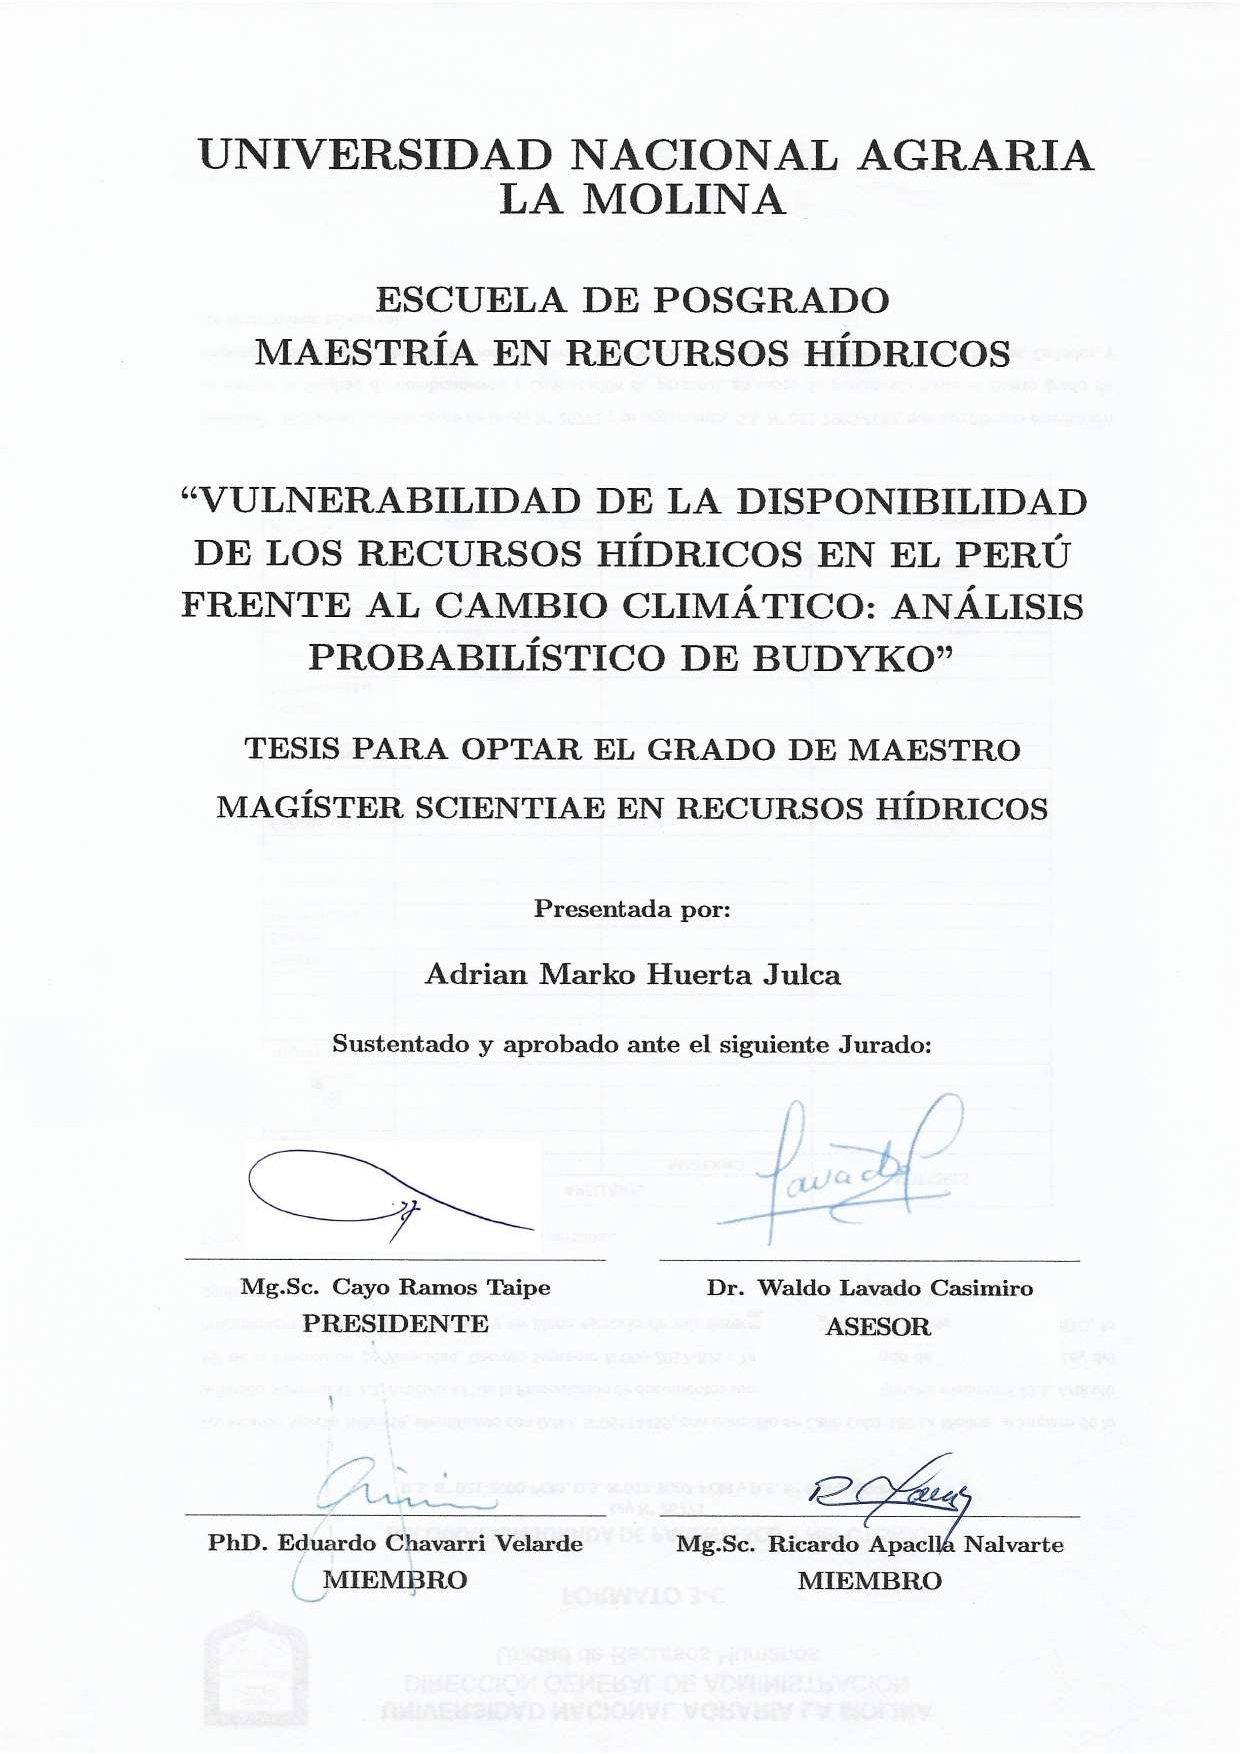
\includepdf[pages=1,fitpaper]{FigsANDTables/firma_jurado}
\clearpage
%=====================  ACTA DE SUSTENTACIÓN ====================
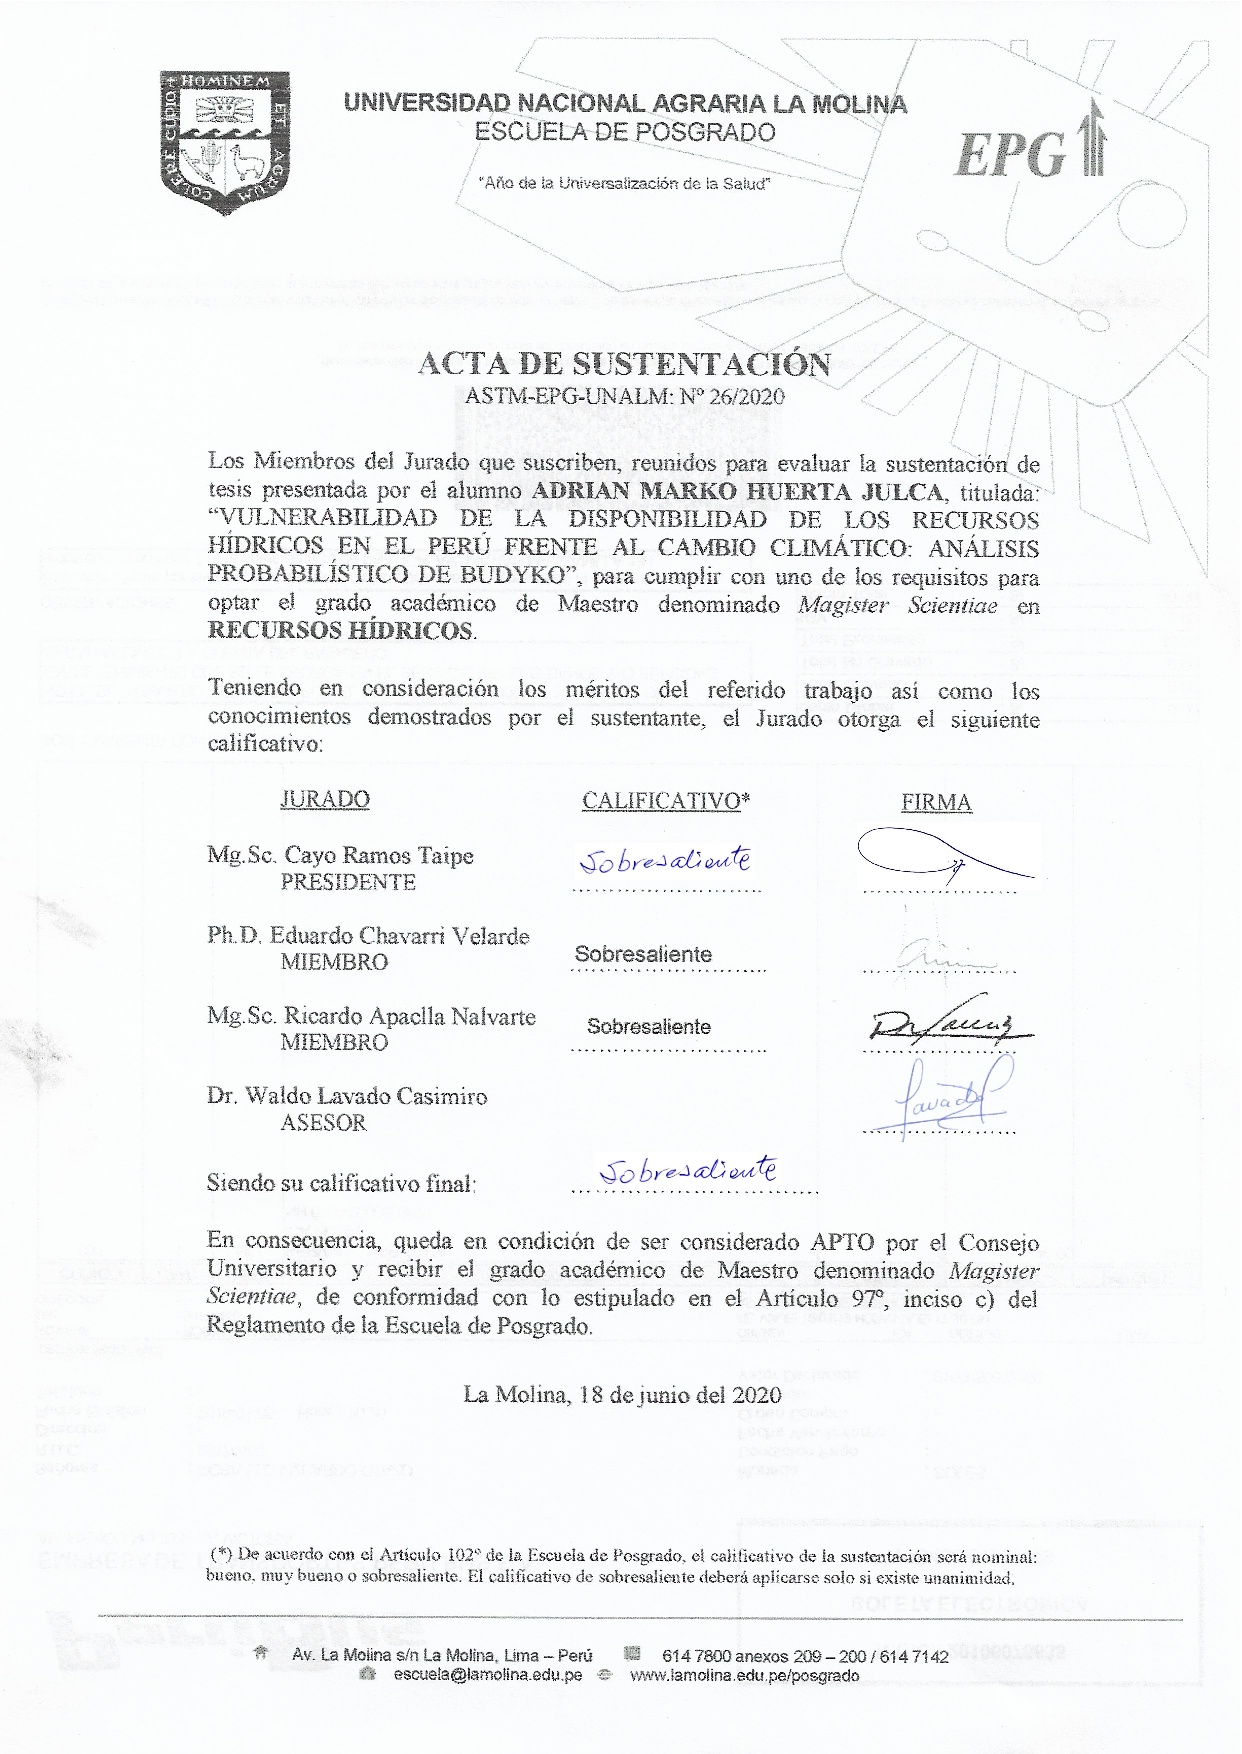
\includepdf[pages=1,fitpaper]{FigsANDTables/acta_sustentacion}
\clearpage
%=====================  DEDICATORIA  =========================
\begin{center}
\large{\textbf {DEDICATORIA}}
\end{center}

\begin{flushright}
A mi abuelo Adriano, a mis padres Jaime y \textit{Luciana}; hermanos y hermanas por su enorme apoyo, esfuerzo y comprensión durante mi segunda etapa de aprendizaje que inició con mis estudios en la Maestría.
\end{flushright}

\clearpage
%=====================  AGRADECIMIENTOS  =========================
\begin{center}
\large{\textbf {AGRADECIMIENTOS}}
\end{center}

\begin{flushright}

La presente investigación se llevó a cabo gracias a la ejecución del Proyecto RAHU con Contrato N$^{\circ}$ 005-2019-FONDECYT “Water Security and Climate Change adaptation in Peruvian glacier-fed rivers basins”, financiado por el Fondo Newton-Paulet, a través de NERC y Fondecyt.\\
Un especial agradecimiento al Dr. Waldo Lavado, quien ha asesorado la investigación, y por las interesantes discusiones y sugerencias. De igual manera a los miembros del jurado (Mg.Sc. Cayo Ramos, PhD. Eduardo Chavarri y Mg.Sc. Ricardo Apaclla) por sus útiles e importantes comentarios.\\
Adicionalmente, a todos los compañeros y amigos de la Maestría y de la Subdirección de Estudios e Investigaciones Hidrológicas (antes Hidrología Aplicada), con quienes compartí inquietudes, conocimientos y momentos muy gratos. Finalmente, pero no por ello menos importante, a mis amigos “meteoros" por los conocimientos compartidos, las aventuras y el apoyo emocional.
\end{flushright}
\clearpage

\tableofcontents
\clearpage
\listoffigures
\clearpage
\listoftables
\clearpage
\listofappendices
\clearpage

%Abreviaturas
%this part is optional, thus I just made it manual, it could be automated
\begin{center}
\large{\textbf {LISTA DE ABREVIATURAS}}
\end{center}

\textbf{IPCC}: Panel Intergubernamental en Cambio Climático \\
\textbf{RH}: Recursos Hídricos \\
\textbf{GCM}: Modelos de Circulación General \\
\textbf{GHG}: Gases de Efecto Invernadero \\
\textbf{P}: Precipitación \\
\textbf{AE}: Evapotranspiración Actual \\
\textbf{Q}: Caudal \\
\textbf{PA}: Evapotranspiración Potencial \\
\textbf{AE/P}: Ratio de Evaporación \\
\textbf{PA/P}: Índice de Aridez \\
\textbf{T}: Temperatura \\
\textbf{Tx}: Temperatura Máxima \\
\textbf{Tn}: Temperatura Mínima \\
\textbf{SENAMHI}: Servicio Nacional de Meteorología de Hidrología del Perú \\
\textbf{PISCO}: Datos Interpolados peruanos de las observaciones climatológicas e hidrológicas del SENAMHI \\
\textbf{PISCOp}: PISCO precipitación \\
\textbf{PISCOt}: PISCO Temperatura \\
\textbf{GLEAM}: Modelo Global de Evaporación Continental de Amsterdam \citep{Martens2017} \\
\textbf{MODIS16}: Proyecto Global de Evapotranspiración MODIS \citep{mu2013modis} \\
\textbf{SSEBop}: Modelo Operativo de Balance de Energía de Superficie Simplificado \\
\textbf{TerraClimate}: Bases de datos climáticos y balance hídrico de \citet{abatzoglou2018terraclimate}\\
\textbf{ZHANG}: Base de Evapotranspiración actual de \citet{zhang2015vegetation} \\
\textbf{MEAN}: Promedio de GLEAM, MODIS16, SSEBop, TerraClimate y ZHANG \\
\textbf{SO-HYBAM}: Observatorio de Investigación Ambiental \\
\textbf{ANA}: Autoridad Nacional del Agua \\
\textbf{UH}: Unidad Hidrográfica \\
\textbf{Td}: Métrica de similaridad \\
\textbf{Rs}: Correlación de Spearman \\
\textbf{RMSE}: Métrica error cuadrático medio \\
\textbf{bias}: Métrica error simple \\
\textbf{WA}: Disponibilidad de los RH \\
\textbf{VI}: Vulnerabilidad de WA \\

\clearpage

\begin{center}
\large{\textbf {RESUMEN}}
\end{center}

Este estudio proporciona por primera vez un análisis de la disponibilidad de los recursos hidricos a escala de cuenca hidrográfica en el Perú. Utilizando nuevos conjuntos de datos grillados de precipitación y temperatura, junto con seis estimaciones reales de evapotranspiración de productos de percepción remota, se evalúo la vulnerabilidad de los recursos hídricos debido al cambio climático. Esto se aborda bajo un enfoque ascendente y un marco probabilístico de Budyko. Primero, se realiza una clasificación de los productos de percepción remota bajo en enfoque de balance hídrico. Luego, se aplica el Budyko probabilístico y se valida de forma cruzada utilizando la inferencia de evapotranspiración real adecuada. Finalmente, la vulnerabilidad del agua y la incertidumbre asociada se calculan a partir del Budyko probabilístico calibrado junto con los espacios climáticos a partir de las variaciones de evapotranspiración potencial (de temperatura) y precipitación. Los principales resultados mostraron que los mejores productos para usar en Perú fueron: GLEAM, MEDIAN, TerraClimate, ZHANG, MODIS16 y SSEBop. Además, el probabilístico Budyko ofreció un buen rendimiento, principalmente en la vertiente hidrográfica del Amazonas. Adicionalmente, las cuencas ubicadas en los Andes, especialmente en el sur, mostraron un menor cambio crítico de precipitación (menos del 10 \%) para aumentar la vulnerabilidad de la disponibilidad de los recursos hídricos en un 25\%.

\textbf {Palabras clave:} Budyko probabilístico, evapotranspiración actual, bottom-up, cambio climático.

\clearpage

\begin{center}
\large{\textbf {ABSTRACT}}
\end{center}

This study provides for the-first-time a water availability analysis at basin-scale in Peru. Using new gridded datasets of precipitation and temperature, along with six actual evapotranspiration estimations from remote sensing products, the vulnerability of water resources due to climate change is evaluated. This is addressed under a bottom-up approach and probabilistic Budyko framework. First, a ranking of remote sensing products is done under a water-balance view. Later, the probabilistic Budyko is applied and cross-validated using the adequated actual evapotranspiration inference. Finally, water vulnerability and associated uncertainty are computed from the calibrated probabilistic Budyko along with climate spaces from variations of potential evapotranspiration (from temperature) and precipitation. The main results showed that the best products to use in Peru were: GLEAM, MEDIAN, TerraClimate, Zhang, MODIS16, and SSEBop. In addition, the probabilistic Budyko provides good performance, mainly in the Amazon River watershed. Furthermore, basins located in the Andes, especially in the southern, showed lower critical precipitation change (less than 10\%) to increase the vulnerability of water availability in 25\%.

\textbf {Key words:} probabilistic Budyko, actual evapotranspiration, bottom-up, climate change.

\clearpage

\pagenumbering{gobble}
\pagenumbering{arabic}

\clearpage
\vspace*{0.5mm}
\section{INTRODUCCIÓN}

El Quinto Reporte del Panel Intergubernamental en Cambio Climático \citep[IPCC;][]{Field2014} indica que el 93\% de los impactos asociados al cambio climático será sobre los recursos hídricos (RH). A escala global ya existe evidencia de perturbaciones en los patrones de precipitación y descargas, impactando en la frecuencia y magnitud de inundaciones y sequías, contribuyendo en un mayor aumento de eventos extremos hidro-climáticos. La disponibilidad de recursos renovables de aguas superficiales y subterráneas probablemente disminuiría en la mayoría de regiones subtropicales áridas y semi-áridas, agravando la oferta de agua para la agricultura, ecosistemas, industria y población \citep{Field2014}. Este escenario es particularmente preocupante en los países en desarrollo del hemisferio sur \citep{Satterthwaite2012} debido a los altos niveles de exposición a los peligros asociados de los RH con el cambio climático, así también por factores no climáticos (sobre-explotación y falta de manejo) \citep{MacAlister2018}.

En Perú, las altas montañas toman un rol importante como fuente de agua para las ciudades y ecosistemas, esencialmente para las zonas bajas áridas adyacentes, porque almacenan y liberan agua de los glaciares y lagos \citep{Coudrain2005,Barnett2005,Viviroli2011}. Estudios concernientes al impacto del cambio climático en recursos hídricos en los Andes Peruanos tienden a estar enfocados en el retroceso glaciar \citep{VUILLE2018195,drenkhan2018current} y su impacto en los caudales, o en determinadas cuencas con información disponible en la que se pueda desarrollar modelos hidrológicos y su proyección futura. Por ejemplo, \citet{Pouyaud2005}, en la cuenca del río Llanganuco utilizó un incremento de temperatura de 0.1 $^{\circ}$C/década encontrando que los caudales en los próximos 20–50 años aumentan debido a la fusión del glaciar, conllevando a que el caudal sea dominado por la precipitación. \citet{Juen2007}, en la misma área de estudio, obtuvo similares resultados con el uso de un modelo hidro-glaciar más sofisticado proyectado con los modelos de circulación general (GCM) de cambio climático. La proyección evidenció una reducción de la estación seca debido a la disminución del tamaño glaciar, así también el periodo húmedo resultó ser más húmedo a causa de escorrentía directa por más lluvia. En el gradiente Andino-Amazónico, \citet{LavadoCasimiro2011} utilizó dos modelos hidrológicos, los datos climáticos de 3 GCM en 2 escenarios de emisión, y encontraron tendencias de descarga tanto decrecientes (4 cuencas) como crecientes (3 cuencas) en las cuencas de la Amazonia peruana. Para la cuenca del río Vilcanota, en los Andes Orientales del Sur del Perú, \citet{Andres2014} mediante la modelización hidrológica de datos satelitales y la aplicación de los GCM encontró que en los próximos cien años habrá más escorrentía total durante la temporada de lluvias (enero a marzo), y menos agua disponible en la estación seca (mayo a octubre). En la cuenca del río Santa, \citet{VanSoesbergen2016} descubre una tendencia hacia el aumento de la disponibilidad de agua debido a la incremento de precipitación, sin embargo, enfatizan la alta incertidumbre de sus resultados. \citet{Olsson2017}, en la cuenca del río Chancay-Huaral, localizado en el Pacífico central, menciona que a razón de los incrementos de precipitación, las descargas de los ríos también aumentaran, esto en mayor medida en el periodo húmedo que en el seco, donde puede haber decrecimiento de acuerdo a ciertos escenarios de emisión. Recientemente, \citet{Pilares2018} evaluó la disponibilidad de agua futura en la cuenca del río Cabanillas, en la vertiente del Lago Titicaca, hallando que solo el 80\% de la demanda es satisfecha, pero que el cambio climático ejerce un efecto sobre los aportes hídricos con un incremento del 15\% al 20\% de la disponibilidad hídrica. 

En general, los anteriores estudios demuestran que la disponibilidad del RH aumenta o no puede cambiar mucho con respecto al presente, así como también cambios significativos en la estacionalidad. No obstante, existen diferencias significativas entre las distintas proyecciones, que conducen a grandes diferencias en los RH entre escenarios \citep{Vuille2008} y son una incertidumbre clave asociada con la evaluación de los impactos del cambio climático en los RH, particularmente en el Perú \citep{VanSoesbergen2016}. Las incertidumbres son inherentes en los GCM debido a la representación simplificada de los mecanismos físicos de nubes, lluvia y topografía. Asimismo, se introduce más incertidumbre cuando se combinan con modelos hidrológicos, ya que las salidas de los GCM deben ser escaladas “downscaling" a una mayor resolución espacial. La resolución generalmente gruesa de los GCM suaviza los gradientes naturales en la precipitación y la temperatura, generando mayores problemas en regiones montañosas, ya que su hidrología se caracteriza por fuertes gradientes de elevación \citep{Buytaert2010}. Entonces para superar la problemática de la información escasa y la incertidumbre inherente de los GCM este estudio propone la combinación de la versión probabilística de la curva de Budyko \citep{Singh2015,Greve2015} con un enfoque de abajo hacia arriba ``bottom-up" para determinar la disponibilidad del RH frente al cambio climático en el Perú. La ventaja del enfoque ``bottom-up" es su independencia de las proyecciones futuras de cambio climático \citep{Singh2014,Poff2016}. Con el enfoque metodológico propuesto se determinará umbrales climáticos críticos de la disponibilidad del RH en todo el país y a diferencia de los anteriores estudios, este ofrece tres principales ventajas: i) una base de datos independiente para comparar estimaciones basadas en datos de caudales y modelos hidrológicos, ii) proporciona la cuantificación de la incertidumbre (no solo del clima, sino de fuentes secundarias) en las estimaciones sobre la disponibilidad de RH, iii) es simple y computacionalmente eficiente, conllevando un aumento potencial de la ayuda a los tomadores de decisiones al estimar los cambios de la disponibilidad de RH en el futuro así como su sensibilidad al cambio climático.

La gran variabilidad espacio-temporal de la oferta de recursos hídricos en el Perú y su rol trascendental en el desarrollo del país para los diferentes sectores así como para la ecología se encuentran vulnerables si se produce un cambio en la cantidad y/o estacionalidad, la cual tendría impactos para diversos sectores como el suministro de agua fresca, agricultura y la generación de energía \citep{barnett2005potential,vergara2007economic,salzmann2009integrated}. En la actualidad, la disponibilidad de los RH en el Perú exhibe patrones espaciales de estrés hídrico por vertientes hidrográficas. Las cuencas de la vertiente del Pacífico solo se benefician del 2\% del total de agua fresca disponible a nivel nacional y concentran casi el 50\% del total de la población \citep{rau2018hydroclimatic}. Por otro lado, el agua es esencial para la producción de alimentos en los Andes peruanos, donde el 80\% de los habitantes dependen de la agricultura como su principal fuente de ingresos \citep{lasage2015stepwise}. La dependencia de los RH se demuestra también por la reducción de la producción agrícola en un 60\% - 70\% durante la sequía de 1982 \citep{zimmerer1999overlapping}. Asimismo, el impacto del fenómeno de El Niño genera sequías e inundaciones al sur y norte del país respectivamente \citep{lavado2014impactos,Huerta2019a}. Si en las condiciones del clima actual ya se tiene un gran desafío de los RH, entonces en un escenario de clima cambiante se necesita aún más investigación. Por lo tanto se justifica conocer la vulnerabilidad de la disponibilidad de los RH frente al cambio climático en todo el Perú. Además, es esencial cuantificar la incertidumbre de las proyecciones y localizar las áreas de mayor susceptibilidad para optimizar el manejo de los RH en el futuro.

La presente tesis tiene como objetivo general determinar la vulnerabilidad de la disponibilidad de los RH frente al cambio climático en Perú. Teniendo como objetivos específicos: i) Selección de productos globales de evapotranspiración actual basada en percepción remota; ii) Aplicación del marco de Budyko probabilístico; y iii) Estimación de la disponibilidad de RH e incertidumbre asociada frente al cambio climático a través del Budyko probabilístico.


\clearpage
\vspace*{0.5mm}
\section{REVISIÓN DE LITERATURA}

\subsection{Cambio Climático}

El clima de una región es simplemente definido como el promedio de las condiciones atmosféricas en un periodo de 30 años. Entonces, el cambio climático sería los cambios en el promedio de las condiciones atmosféricas en un largo periodo de tiempo también. De acuerdo a la IPCC \citep{IPCC2007}, el cambio climático es determinado como ``el cambio en el estado del clima que puede ser identificado por cambios en el promedio y/o la variabilidad de sus propiedades, y persistir por un extenso periodo de tiempo, normalmente décadas o más”.

El clima ha cambiado a lo largo de la historia de la tierra debido a cambios en sus forzantes naturales y/o antropogénicos. La concentración de gases de efecto invernadero (GHG), los aerosoles, la actividad volcánica y la radiación solar son los motores de cambio más dominantes en los últimos 2000 años \citep{NRC2006}. Los principales gases de efecto invernadero relacionados con el cambio climático son el dióxido de carbono (CO$_{2}$), el metano (CH$_{4}$) y el óxido nitroso (N$_{2}$O). Estos GHG se originan tanto en fuentes naturales (por ejemplo, emisiones volcánicas e incendios forestales) como en fuentes con influencia humana (por ejemplo, la quema de combustibles fósiles y la deforestación). Según \citet{Solomon2007}, los GHG brindan una explicación sólida para la mayoría de las tendencias de calentamiento global y local en las últimas décadas. Se espera que el cambio climático afecte la precipitación y los patrones de evapotranspiración \citep{Tsanis2011} y, en consecuencia, la disponibilidad de agua local, la descarga de ríos y la disponibilidad estacional de suministro de agua \citep{Arnell2011}. 
\clearpage
A escala mundial, la demanda de los RH ha aumentado debido a varios factores como el crecimiento de la población, la contaminación del agua, el progreso económico, el uso de la tierra y el cambio climático, lo cual reduce la disponibilidad de RH en condiciones de un futuro incierto \citep{Davies2011}. Desde el punto de vista socio ambiental, que incluyen la agricultura, el turismo y la conservación de la biodiversidad, la calidad y cantidad de los RH es evaluable, por lo que las medidas de adaptación para el sector del agua están inevitablemente vinculadas con las políticas en diversos campos \citep{Field2014}. También se espera que el cambio climático intensifique el ciclo hidrológico mundial, lo que tendrá como resultado impactos directos en la disponibilidad general de los recursos hídricos para usos domésticos y agrícolas \citep{Huntington2006}. A escala local, las intensidades de lluvia se verán afectadas, lo que provocará inundaciones en las riberas de los ríos más continuamente \citep{Wilby2010}.

\subsection{Vulnerabilidad}

De acuerdo a la IPCC, la vulnerabilidad puede ser definida como el grado en que un sistema es susceptible y no puede hacer frente a los efectos adversos del cambio climático, incluida la variabilidad climática y los extremos. La vulnerabilidad es una función del carácter, la magnitud y la tasa de cambio climático y la variación a la que está expuesto un sistema (social-ecológico), su sensibilidad y su capacidad de adaptación \citep{parry2007climate}.

\citet{nelitz2013tools} menciona que la vulnerabilidad depende de las dimensiones de exposición, sensibilidad y capacidad de adaptación que pueden medirse cuantitativamente o caracterizarse cualitativamente. Estas dimensiones o medidas son \citep{glick2011scanning,fussel2006climate}:

\begin{itemize}
    \item Exposición: mide la magnitud y extensión (espacial y temporal) de la exposición de los impactos al clima (variabilidad y cambio).
    \item Sensibilidad: mide la probabilidad de un sistema como respuesta al estrés inducido por el clima (variabilidad y o cambio).
    \item Capacidad de adaptación: mide la capacidad u oportunidad disponible para disminuir la exposición o sensibilidad de un sistema a un estrés inducido por clima (variabilidad y/o cambio)
\end{itemize}

A partir de la previa caracterización, es posible clasificar y de esta manera catalogar a mas detalle la vulnerabilidad. \citet{nelitz2013tools} define estos elementos tomando en consideración la evaluación de la vulnerabilidad en cuencas hidrográficas (Figura \ref{fig:Nelitz01}).

Evaluar la vulnerabilidad hace referencia a evaluar estos procesos, es decir medir y/o caracterizar la exposición, sensibilidad y la capacidad de adaptación de un sistema natural o humano a perturbar. Para este propósito existen diferentes tratamientos con finalidades especificas. \citet{nelitz2013tools} describe dos ordenes de evaluación de la vulnerabilidad:

\begin{itemize}
    \item Primer orden: evaluación de impacto con la adición de consideraciones socio-económicas y factores no climáticos.
    \item Segundo orden: evaluación de vulnerabilidad de primer orden y mas de la evaluación de la capacidad de adaptación. Este planteamiento asume que los sistemas humanos y ecológicos tienen la capacidad de apaciguar los efectos del clima (cambio y variabilidad).
\end{itemize}

El rango de técnicas y/o herramientas para evaluar la vulnerabilidad de los recursos hídricos se engloba en dos principales enfoques: “top-down" y “bottom-up". Estos son detallados en la siguiente sección.

\begin{sidewaysfigure}
	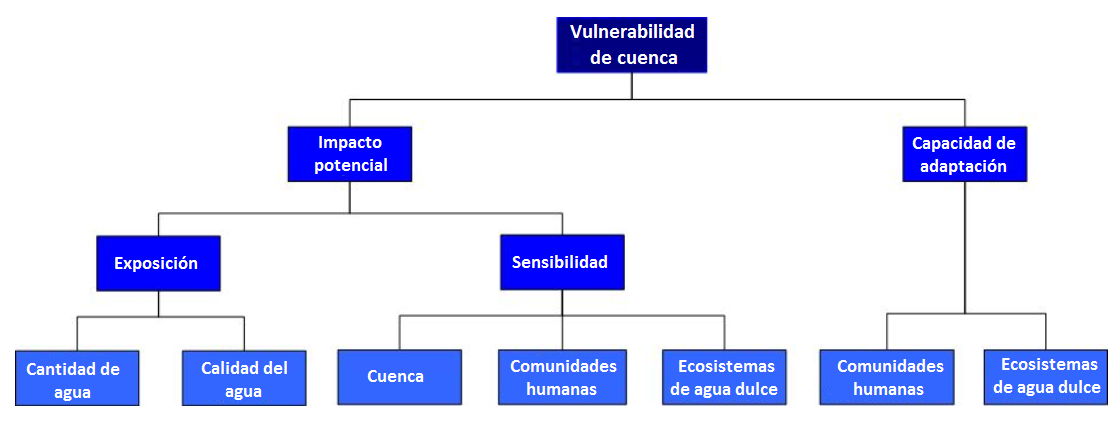
\includegraphics[scale=0.8]{Images/Nelitz01.png}
	\centering
	\caption{Elementos de la evaluación de vulnerabilidad en una cuenca hidrográfica.}
	Fuente: \citet{nelitz2013tools}.
    \label{fig:Nelitz01}
\end{sidewaysfigure}


\subsection{Enfoques de evaluación/adaptación de la vulnerabilidad al cambio climático}

De acuerdo a \citet{Wilby2010} existen dos perspectivas principales sobre la evaluación del riesgo climático para la adaptación. Estos son denominados: de arriba hacia abajo (“top-down", conocidos como ``guiados por escenarios") y de abajo hacia arriba (“bottom-up").

El enfoque “top-down" implica en primer lugar reducir las proyecciones climáticas de los GCM a un rango de escenarios. Los escenarios locales resultantes luego se incorporan a los modelos de impacto (para estimar, por ejemplo, caudales futuros mediante modelos hidrológicos), antes de proceder finalmente en medidas de adaptación para maximizar cualquier beneficio o contrarrestar los riesgos anticipados. El término de “arriba hacia abajo” se usa porque la información se coloca en cascada de un paso a otro, con el número de permutaciones del escenario de emisión, el modelo climático, el método de reducción de escala, etc., que prolifera en cada etapa (Figura \ref{fig:tpbu}). 

Este es el enfoque más utilizado dentro de la evidencia científica del IPCC, y hay muy pocos ejemplos tangibles de decisiones de adaptación anticipada o planificada que surjan de este enfoque. La gran mayoría de los estudios de investigación se detienen en la etapa de evaluación de impacto. Esto posiblemente debido al rango de incertidumbres que se expande en cada paso del proceso en la medida en que los impactos potenciales y sus respuestas de adaptación implícitas abarcan un rango tan amplio que resulta prácticamente de poca utilidad. También existe el peligro de que las proyecciones se perciban como probabilidades reales de cambio cuando, de hecho, las distribuciones resultantes de los cambios de temperatura y precipitación dependen en gran medida del diseño experimental \citep{Dessai2004}. 

\begin{figure}[t]
	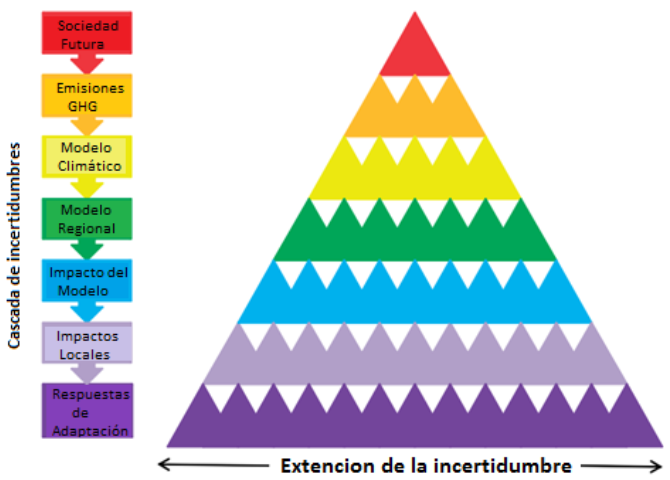
\includegraphics[scale=.64]{Images/tpbu.png}
	\centering
	\caption{Cascada de incertidumbre es estudios de cambio climático.}
    Fuente: \citet{Wilby2010}.
    \label{fig:tpbu}
\end{figure}

La perspectiva “bottom-up" se centran en reducir la vulnerabilidad a la variabilidad climática pasada y presente, generalmente después de un evento extremo o desastre. El término de “abajo hacia arriba" se usa porque el análisis comienza con los factores y condiciones que permiten enfrentar con éxito las amenazas relacionadas con el clima a nivel de individuos, hogares y comunidades. Si bien estas respuestas no dependen de los escenarios de cambio climático, se necesitan observaciones lo suficientemente largas para evaluar las magnitudes y frecuencias de los eventos extremos, así como sus consecuencias sociales y/o ambientales asociadas como la ola de calor en Europa \citep{Palutikof2004}. Sin embargo, existe el peligro de que los medios locales no informen demasiado sobre los eventos extremos.

En la práctica, la vulnerabilidad climática está determinada por una serie de factores que incluyen variaciones en la riqueza, la igualdad social, la disponibilidad de alimentos, el estado de salud y educación, la infraestructura física e institucional, el acceso a los recursos naturales y la tecnología \citep{Brooks2005}. Los indicadores de vulnerabilidad pueden ser útiles para rastrear los cambios en la exposición al riesgo climático y la efectividad de las estrategias de adaptación a lo largo del tiempo; así como también a orientar los recursos en los puntos de mayor susceptibilidad. La adaptación se produce al mejorar las estrategias de afrontamiento o al reducir la exposición a amenazas conocidas.

El propósito de estos enfoques radica en generar información de la vulnerabilidad al cambio climático en el contexto de recursos hídricos (cuencas hidrográficas). El conocimiento generado por una evaluación de vulnerabilidad se utiliza para informar la asignación de recursos para la planificación y adaptación al cambio climático \citep{nelitz2013tools,Dessai2004}. 

\subsection{Evapotranspiración actual}

De acuerdo a \citet{wang2012review}, la evapotranspiración terrestre (evapotranspiración actual, $AE$), es el agua transferida desde la superficie terrestre a la atmósfera. Este intercambio de agua generalmente implica un cambio de fase (del agua) de líquido (o hielo) a gas, que absorbe energía y enfría la superficie de la tierra. El calor latente que acompaña a $AE$ es $\lambda E$, donde $\lambda$ es el calor latente de vaporización. Estos términos son necesarios para los modelos numéricos de predicción meteorológica a corto plazo y para las simulaciones climáticas a más largo plazo y/o para el diagnóstico del cambio climático. En tales modelos, $AE$ generalmente se parametriza como la suma de la evaporación del suelo, la evaporación de la vegetación y la transpiración de la vegetación; este último es un proceso que se combina con la absorción de carbono a través de la fotosíntesis.

El agua es transferida de la superficie terrestre a la atmósfera a través de turbulencias, que puede ser definido como remolinos irregulares de aire de diferentes tamaños superpuestos entre si (Figura \ref{fig:wang01}), y que tienen la capacidad de transportar tales cantidades en comparación a la difusión molecular. En días de mayor radiación, estos remolinos tienden a tener mayor magnitud (aire ascendente) debido al calentamiento del suelo. Su tamaño diverge tanto en la horizontal como vertical. 

\begin{figure}[ht!]
\centering
	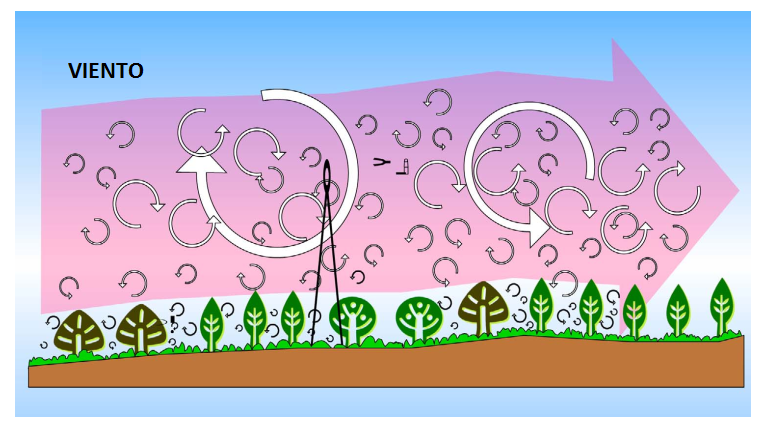
\includegraphics[scale=0.77]{Images/wang01.png}
	\caption{Vista esquemática del flujo de aire que pude ser visto como un flujo horizontal de numerosos remolinos giratorios, es decir, vórtices turbulentos de varios tamaños (con componentes horizontales y verticales).}
	Fuente: \citet{wang2012review}.	
	\label{fig:wang01}
\end{figure}


El agua no solo se transfiere aerodinámicamente, si no también mediante procesos biológicos. La transpiración, es la evaporación del agua en el sistema vascular de las plantas con perdidas por medio de las estomas de las hojas. Según \citet{dirmeyer2006gswp} y \citet{lawrence2007partitioning}, este proceso contribuye en mayor medida al $AE$ total, y esta relacionado con la absorción del carbono en la hoja a través de la conductancia de la misma.

\begin{figure}[ht!]
\centering
	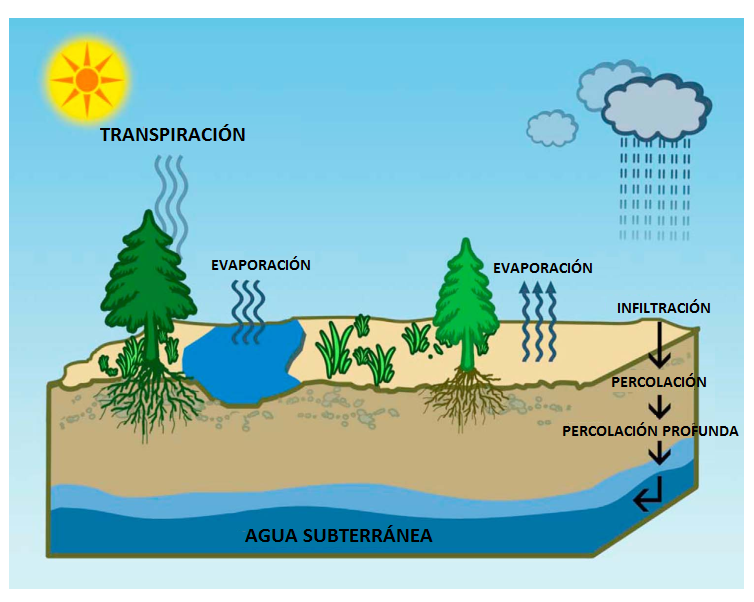
\includegraphics[scale=0.75]{Images/wang02.png}
	\caption{Vista esquemática del proceso de evapotranspiración que incluye transpiración de las hojas y la evaporación del agua.}
	Fuente: \citet{wang2012review}.
	\label{fig:wang02}
\end{figure}

\citet{wang2012review} menciona que una de las primeras teorías en abordar $AE$ fue aquella desarrollado por \citet{monin1954basic} en los 1950s denominado Teoría de la similitud de Monin-Obukhov (MOST). Fue uno de los primeros en relacionar $AE$ y los flujos de calor sensible a partir de mediciones de vientos, temperatura y humedad cercanos a la superficie al enlazar los flujos de turbulencia con los gradientes de viento, temperatura y humedad. Adicionalmente, la ecuación de Penman-Montiet \citep{penman1948natural,monteith1965evaporation} que usa radiación de superficie, temperatura y humedad para estimar $AE$. La ecuación de Penman describe la evaporación de una superficie de agua abierta o de vegetación corta. Según \citet{wang2012review}, la ecuación de Penman puede ser vista como una combinación de MOST y el balance de energía de superficie (SEB). Para un mayor detalla de estas definiciones, revisar \citet{wang2012review}. Otra emergente teoría, mencionada por \citet{zhang2016review}, es la Teoría de Máxima Producción de Entropía (MEP) que explica la termodinámica del no equilibrio y proporciona nuevos enfoques para estimar los flujos de superficie. MEP es derivada del principio de máxima entropía formulado primero como un método general para asignar distribuciones de probabilidad en mecánica estadística. Revisar \citet{zhang2016review} para un mayor entendimiento del enfoque. 

Considerando lo mencionado, se evidencia que $AE$ es un proceso controlado por la combinación de factores físicos y biológicos. Por lo tanto los relativos impactos de los diferentes procesos en $AE$ varían en el tiempo y espacio. A escala global, \citet{zhang2015vegetation} separa $AE$ en tres factores independientes: demanda (en función de la temperatura del aire, humedad y velocidad del viento), suministro (en función de la precipitación) y energía (en función de la radiación y nubosidad). Los resultados de \citet{zhang2015vegetation} (Figura \ref{fig:zhang_rev01}) resaltaron que el suministro de agua influye mas en $AE$ en 49\% del área de la tierra, principalmente en regiones áridas y semi-áridas. La energía disponible domina en un 32\%, específicamente en regiones de clima húmedo tropical y en latitudes altas del norte. La demanda de agua atmosférica es el factor de control dominante en más del 19\% del mundo, principalmente en áreas de alta montaña y latitudes altas. 

\begin{figure}[ht!]
\centering
	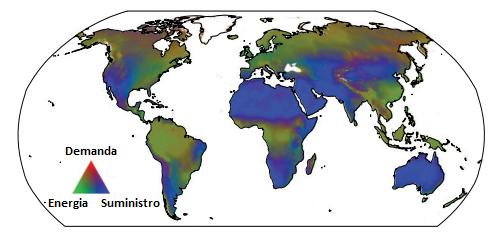
\includegraphics[scale=1]{Images/zhang_rev01.png}
	\caption{Distribución geográfica de los factores climáticos primarios que regulan la evapotranspiración. Demanda = (temperatura del aire, humedad, velocidad del viento), Suministro = (precipitación) y Energía = (radiación y nubosidad)}
	Fuente: \citet{zhang2015vegetation}.
	\label{fig:zhang_rev01}
\end{figure}

\subsubsection{Observaciones de evapotranspiración actual}

\citet{wang2012review} caracteriza los principales métodos de observación y estimación de $AE$ que puede usarse para proporcionar observación a largo plazo. Estas se encuentra resumidas en la Tabla \ref{tab:TableZhang01}. La versión completa de la Tabla \ref{tab:TableZhang01} puede ser revisada en \citet{wang2012review}.
 
\begin{table}[ht]
\caption{Resumen de observaciones y estimaciones de evapotranspiración. mh: media hora, M: mensual, y A: anual}
\vspace{.2cm}
\label{tab:TableZhang01}
\centering
\begin{tabular}{l|l|l|l}
\hline
\textbf{Método} & \textbf{Escala}   & \textbf{Escala}             & \textbf{Ventajas}         \\
                & \textbf{temporal} & \textbf{espacial}           &                           \\ \hline
Eddy            & mh - A            & cientos de metros           & medición directa de       \\
covariance      &                   & en función de la            & los flujos de turbulencia \\
                &                   & altura de medición por      & observación de energía    \\ \cline{1-2}
Relación           & mh - A            & encima de la capa del dosel & independiente             \\
de Bowen        &                   & y la velocidad del viento   & es equilibrada            \\ \hline
Lisímetro       & mh - A            & punto de medición           & observación directa       \\ \cline{1-3}
Cintilómetro    & mh - A            & decenas de metros a         & estimación a              \\
                &                   & decenas de kilómetros       & grandes escalas           \\ \hline
Balance         & M - A             &                             & estimación directa        \\
hídrico         &                   & cientos                     & estimación regional       \\
superficial    &                   & a miles                     & y global                  \\ \cline{1-2} \cline{4-4} 
Balance         & M - A             & de kilómetros               & estimación regional       \\
atmosférico     &                   &                             & y global                  \\ \hline
\end{tabular}
\end{table}
\vspace*{-.5cm}
Fuente: \citet{wang2012review}.



\subsubsection{Observaciones basados en percepción remota}

Debido a la rentabilidad, amplia cobertura, reproducibilidad y moderada a alta precisión, la estimación de $AE$ por percepción remota ha sido utilizada como principal fuente de información y área de estudio en las ultimas décadas. De acuerdo a \citet{zhang2016review}, la estimación de $AE$ basada en percepción remota comenzó aproximadamente en la década de los 1980s y ha evolucionado a una gran variedad de orientaciones y modelos. Es evidente que no existe un consenso de cual enfoque/método es mejor ya que cada uno presentan ventajas y desventajas. 

Un resumen de las diferentes técnicas fueron provistas en \citet{zhang2016review}, y una versión simplificada se encuentra en la Tabla \ref{tab:TableZhang02}. Para un mayor entendimiento de la Tabla \ref{tab:TableZhang02}, los acrónimos usados en la misma hacen referencia al índice de temperatura superficial-vegetación (LST-VI), Penman-Monteith \citep[P-M;][]{penman1948natural,monteith1965evaporation} y Priestley-Taylor \citep[PT;][]{priestley1972assessment}.

\vspace{.5cm}
% Please add the following required packages to your document preamble:
% \usepackage{longtable}
% Note: It may be necessary to compile the document several times to get a multi-page table to line up properly
\begin{longtable}{l|l|l}
\caption{Resumen de los principales métodos de estimación de evapotranspiración actual basado en percepción remota. \label{tab:TableZhang02}} \\
\hline
\textbf{Método} & \textbf{Ventajas}        & \textbf{Asunciones y/o}             \\
\endfirsthead
%
\multicolumn{3}{c}%
{{\textbf{$<<$continuación$>>$} \vspace{.5cm}}} \\
\endhead
%
\hline
\endfoot
%
\endlastfoot
%
\textbf{}       & \textbf{}                & \textbf{limitaciones}               \\ \hline
SEB             &                          & Solo para cielo despejado;          \\
Una fuente      & Simple, y poco           & requiere excesiva                   \\
                & requerimiento de         & parametrización de                  \\ \cline{1-1}
SEB             & información              & resistencia y calibración local;    \\
Una fuente con  & meteorológica            & probable a errores de $LST$ y $T$;      \\
variabilidad    &                          & requiere valores            \\
espacial        &                          & instantáneos a diarios              \\ \hline
SEB             &                          &                                     \\
Dos fuentes     & Poco requerimiento       & Solo para cielo despejado;          \\ \cline{1-1}
SEB             & de información           & muy sensible a los errores de $LST$;   \\
Dos fuentes     &  meteorológica           & requiere valores          \\
(tiempo         &                          & instantáneos a diarios              \\
diferenciado)   &                          &                                     \\ \hline
LST-VI          & Poco requerimiento      & Solo  para cielo despejado;         \\
                & de información           & Relación LST-VI muy simplificado;   \\
                & bajo impacto en          &   requiere valores                  \\
                & errores de $LST$         & instantáneos a diario     \\ \hline
PM              & Cobertura continua       & Alto requerimiento de datos;          \\
                & basada en procesos       & Estimación simplificada o           \\
                & físicos.                  & semi-empírica de la                 \\
                & Paso de tiempo flexible, & conductancia del dosel              \\
                & sin requisitos o con     &                                     \\
                & requisitos bajos de $LST$  &                                     \\ \hline
PT              & Simple; requerimiento    & Muchas simplificaciones físicas;     \\
                & moderado de              & requiere flujo de calor del suelo   \\
                & información              & como entrada o supone que           \\
                &                          & es despreciable; aplicado             \\ 
                &                          & a escala mensual                    \\ \hline
MEP             & Poca información         & Requiere $LST$ continuo para            \\
                & meteorológica            & producir un registro $AE$ continuo.     \\ \hline
Balance         & Simple y fácil           & No puede derivar directamente $AE$;    \\
Hídrico         & de aplicar               & pobre resolución espacio-temporal   \\
                &                          & sensible a los errores de $P$         \\ \hline
Agua -          & Considerando relación    & Posible requerimiento de mucha      \\
Carbono         & entre el carbono y       & información, afectado por           \\
                & flujos de agua           & vacíos y/o errores.                  \\ \hline
Modelos         & simple y fácil           & Requiere calibración y capacidad     \\
Empíricos       & de aplicar               & baja fuera del área de calibración; \\
                &                          & proceso físico simplificado;      \\
                &                          & sujeto a condiciones climáticas     \\
                &                          & si se requiere $LST$                   \\ \hline
\end{longtable}
\vspace*{-1.25cm}
FUENTE: \citet{zhang2016review}



\subsection{Enfoque de Budyko}

El enfoque de Budyko \citep{Budyko1961,Pike1964} descrita en \citet{Zhang2008} está basado en la ecuación de balance:

\begin{equation}
\frac{\partial S(t)}{\partial t} = P(t) - AE(t) - Q(t) 
\end{equation}

Donde, $\frac{\partial S(t)}{\partial t}$ es el cambio en el paso de tiempo $t$, $P$ es la precipitación o llegada de agua, $AE$ es la evapotranspiración actual y $Q$ es el caudal. Si la ecuación es integrada sobre un periodo de tiempo suficientemente largo (muchos años o décadas), el balance hídrico se convierte una ecuación de equilibrio. El cambio neto en el almacenamiento durante este período de tiempo será cero ($\Delta S = 0$) para que el agua entrante con el tiempo, sea equilibrado por el agua saliente:

\begin{equation}
\overline{P} = \overline{AE} + \overline{Q} 
\label{equ:WB}
\end{equation}

Para la estimación del promedio de $\overline{AE}$, \citet{Budyko1961} razono que $\overline{AE}$ seria menor que el agua disponible ($\overline{P}$) y de la disponibilidad de energía para la evaporación ($\overline{R}/\lambda$, donde $\overline{R}$ es la radiación y $\lambda$ la vaporización latente del agua):

\begin{equation}
\overline{AE} \leq min(\overline{P}, \frac{\overline{R}}{\lambda })
\end{equation}

Él asumió también que la precipitación y energía fueron los factores más dominantes en la evaporación. Denomino $\overline{R}/\overline{P}\lambda$ como el índice de aridez denotado por $\phi$, y desarrollo una relación entre $\overline{R}$ y el índice de aridez:

\begin{equation}
\phi = \frac{\overline{R}}{\overline{P}\lambda}
\end{equation}

\begin{equation}
\overline{AE} = \left [ \phi\left ( tan\frac{1}{\phi}  \right )1 - cos\phi + sen\phi \right ]^{0.5}
\end{equation}

Un problema con este método, es la falta de capacidad de tomar otros factores además del índice de aridez. \citet{Fu1981} desarrollo un método similar a Budyko para estimar la evapotranspiración actual anual media $\overline{AE}$, de la precipitación $\overline{P}$ y evapotranspiración potencial $\overline{PA}$ promedio anual, e introdujo un factor de partición $\omega$: 

\begin{equation}
\frac{\overline{AE}}{\overline{P}} = 1 + \frac{\overline{PE}}{\overline{P}} - \left (1 + \left ( \frac{\overline{PE}}{\overline{P}} \right )^{\omega}  \right )^{1/\omega}
\label{equ:fuEqu}
\end{equation}

Donde $\omega$ tiene el rango de $[1,\infty)$. La ecuación de \citet{Fu1981} hace posible definir diferentes relaciones entre $\overline{AE}/\overline{PE}$ y $\overline{PE}/\overline{P}$ para diferentes regiones, solo variando $\omega$. \citet{Fu1981} usa $\overline{PE}/\overline{P}$ como el índice de aridez en vez de $\overline{R}/\overline{P}\lambda$, pero los dos son esencialmente similar como la radiación $R$ es el principal conductor de la evapotranspiración potencial $\overline{PE}$.

\citet{Koster1999} aplicaron satisfactoriamente la relación de Budyko entre $\overline{AE}$ y el índice de aridez $\phi$ a escalas inter-anuales, bajo el supuesto que los cambios a esa escala en el almacenamiento son mucho menor que los flujos. Para escalas de tiempo menor (sub-anual o menor), la situación de equilibrio no es aplicable, y los cambios en el almacenamiento debe ser considerada. \citet{Zhang2008}, aplico la ecuación de Fu a intervalos tanto diarios y mensuales, ya no bajo el supuesto de estado estable, sino al incluir cambios de almacenamiento. El modelo calibración de \citet{Zhang2008} define $\alpha = 1 - 1/\omega$ , donde el rango de $\alpha$ es $[0,1)$ (Figura \ref{fig:budyko00}):

\begin{equation}
\frac{\overline{AE}}{\overline{P}} = 1 + \frac{\overline{PE}}{\overline{P}} - \left (1 + \left ( \frac{\overline{PE}}{\overline{P}} \right )^{1/1-\alpha}  \right )^{1-\alpha}
\label{equ:eq7}
\end{equation}

\begin{figure}[ht]
	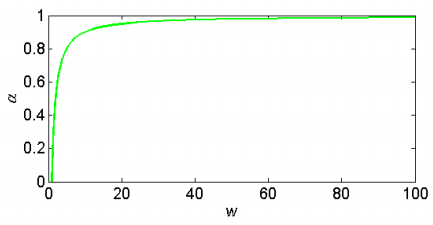
\includegraphics[scale=1]{Images/budyko00.png}
	\centering
	\caption{$\alpha$ en función de $\omega$ como fue definido en \citet{Zhang2008} para el propósito de calibración.}
	{\raggedright FUENTE: \citet{Krogh2011}. \par}

	\label{fig:budyko00}
\end{figure}



La Ecuación \ref{equ:eq7} no utilizo promedio temporales ya que el estado estacionario no es una suposición. La Figura \ref{fig:budyko01} muestra el ratio de evaporación $AE/P$ como función del índice de aridez, a diferentes valores de $\alpha$, así como la curva original de Budyko de $AE/P$. Valores altos de $\alpha$ corresponden a una alta eficiencia de evapotranspiración, por lo tanto, cuanto más cercano $\alpha$ sea a 1, más cerca estará el $AE$ del límite de demanda ($PE$) o del límite de suministro ($P$); mientras que un bajo $\alpha$ dará un $AE$ bajo.

\begin{figure}[ht!]
	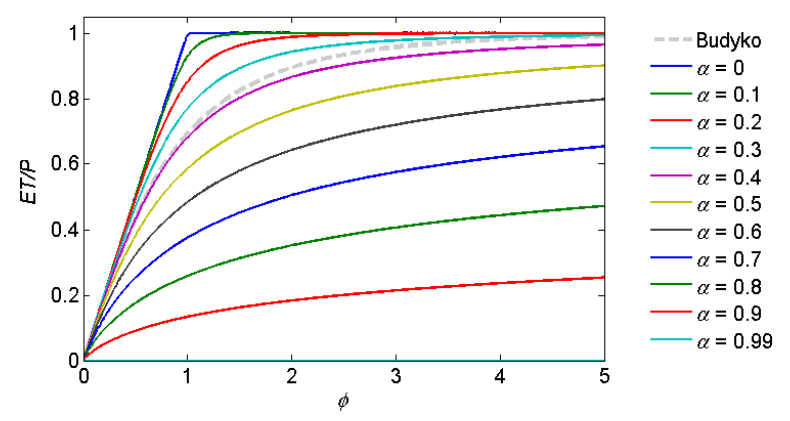
\includegraphics[scale=.57]{Images/budyko01.png}
	\centering
	\caption{Relación de $AE/P$ en función del índice de aridez para diferentes a valores de acuerdo a la ecuación de \citet{Fu1981}.}
	Fuente: \citet{Krogh2011}.
	\label{fig:budyko01}
\end{figure}

 

\subsubsection{Budyko probabilístico}

En el marco original de Budyko, las condiciones climáticas están expresadas en términos de $PE/P$ y $AE/P$. Esta relación no es lineal y presenta limites físicos, denominados: la demanda de agua atmosférica ($AE < P$) y suministro de agua atmosférica ($AE < PE$) (Figuras \ref{fig:budyko01} y \ref{fig:Greve01}). Como se ha presentado en la sección anterior, la curva original de Budyko es enteramente determinista y no paramétrica, y ha presentado diversas modificaciones y variaciones a lo largo de los años \citep{Budyko1961,Fu1981,Koster1999,Wang2014,Zhang2004,Zhang2008,fathi2019new}. 

\vspace{.25cm}
\begin{figure}[ht!]
\centering
	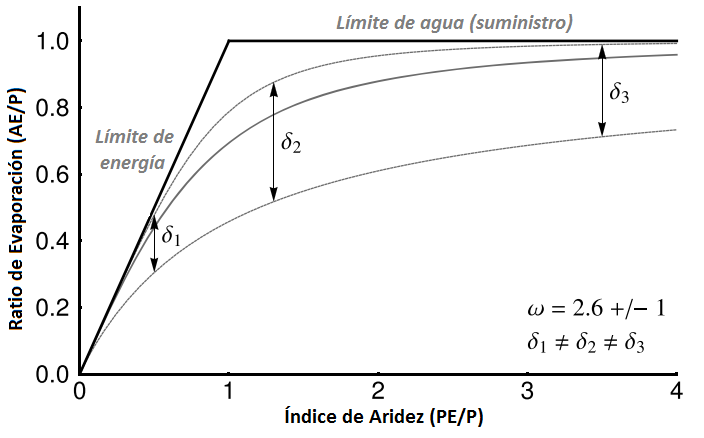
\includegraphics[scale=0.7]{Images/Greve2015_original_budyko.png}
	\caption{Tradicional curva de Budyko (correspondiente a un $\omega = 2.6$ \citep{Fu1981,Zhang2004}, linea gris) ubicando por $\omega = 2.6 \pm 1$ (lineas delgadas). La distancia Euclidiana ($\delta$) entre las curvas es diferente para cada valor de $PE/P$.}
	{\raggedright FUENTE: \citet{Greve2015}. \par}
	\label{fig:Greve01}
\end{figure}


El parámetro $\omega$ (de \citet{Fu1981}, Ecuación \ref{equ:fuEqu}) no tiene significado físico a priori, sin embargo, es usualmente interpretado como una propiedad integradora de todas las características de captación y del clima (por ejemplo, ciclo estacional) que no sean las condiciones climáticas medias prevalecientes (expresadas en términos de $PE/P$ y $AE/P$), incluidas las propiedades de vegetación, geográficas, topográficas y del suelo \citep{Gentine2012,Berghuijs2014,Greve2015}. A pesar de los esfuerzos en la búsqueda de una interpretación integral de $\omega$, aun no se ha llegado a ideas definitivas sobre sus influencias (factores que controlan).

En este sentido, \citet{Greve2015} motivado por la falta de explicación sobre la no linealidad del espacio de fases (de la curva) y el consecuente uso problemático de las medidas de distancia euclidiana (Figura \ref{fig:Greve01}), establece el marco probabilístico de Budyko. Este nuevo enfoque permite la estimación en forma de distribución del  valor de $AE/P$ para un $PE/P$ dado, en comparación a uno solo, así como también cuantificar la curva media en un sentido probabilístico.

\paragraph{Teoria}\mbox{}

\citet{Greve2015} estableció la representación probabilística del enfoque de Budyko basado en la Ecuación \ref{equ:fuEqu} de \citet{Fu1981}. El parámetro $\omega$ es un parámetro matematico necesario para la solución dentro del espacio de Budyko, y no tiene significado físico a priori. Entonces, por definición $\omega \in]1,\infty ]$ y cada punto dentro de los limites (del espacio) puede ser asignado a un $\omega$ especifico. Bajo condiciones reales, el valor mínimo de $\omega$ no es necesariamente 1, puede ser mayor \citet{Zhang2004}. 

El valor de $\omega$ es diverso en los diferentes estudios aplicados y difiere entre cuencas. En la actualidad, aun no se ha identificado su principal influencia. Por lo tanto, \citet{Greve2015} hipotetizo que la combinación integradora de todas las influencias de la cuenca y el clima (excepto de $PE/P$) en $\omega$ puede ser caracterizado como un proceso estocástico, asumiendo que $\omega$ sigue una determinada distribución: $\omega \sim D(\textbf{p})$ con $D$ siendo una distribución arbitraria con cola inferior limitado a 1 (por $\omega \in]1,\infty ]$, siendo cualquiera) y $\textbf{p}$ los parámetros de la distribución. Dado esto, es entonces posible obtener una distribución de $AE/P$ para un $PE/P$ dado que depende de los parámetros de la distribución especifica $D(\textbf{p})$ para $\omega$. 
Ya que no existe una solución analítica factible para la función de densidad de probabilidad de $AE/P$, \citet{Greve2015} propuso una solución mediante simulación estocástica (siguiendo el enfoque de Monte Carlo). Entonces, para un numero grande de simulaciones, $n$ variables aleatorias $y_{n} = AE/P$ fueron generadas de la Ecuación \ref{equ:fuEqu} para un $x = PE/P$ asumiendo $\omega \sim D(\textbf{p})$. Las propiedades de la distribución (mediana, momentos, cuantiles, etc) de Budyko fueron estimados directamente de la simulación de distribución o del estimado mediante la técnica de kernel (si el $n$ de simulaciones fue pequeña).

\vspace{.25cm}
\begin{figure}[ht!]
\centering
	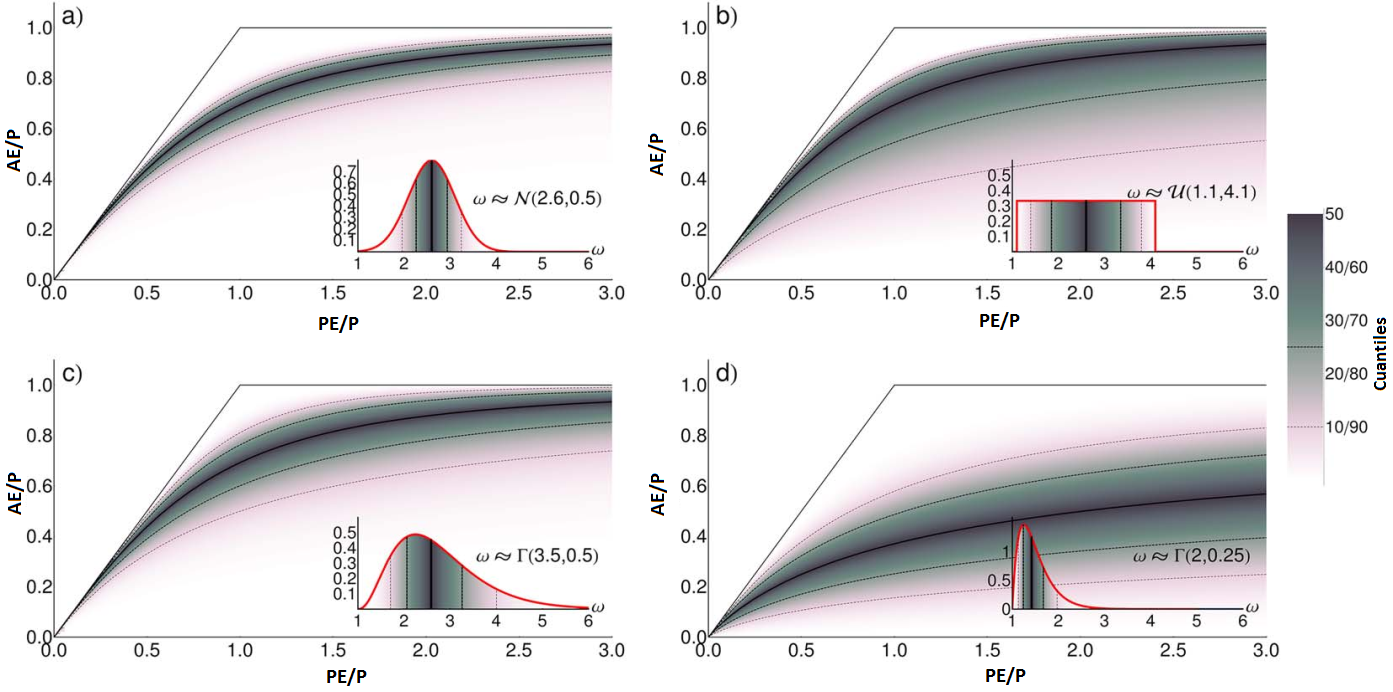
\includegraphics[scale=0.35]{Images/Greve02.png}
	\caption{Enfoque de Budyko probabilístico con un $\omega$ siguiendo a) una distribución normal truncada, b) una distribución uniforme y (c y d) dos diferentes distribuciones gamma. Las distribuciones de a, b y c muestran una mediana comuna $\omega = 2.6$, que corresponde al Budyko original (linea negras solida). Los respectivos cuantiles se muestran como sombras.}
	{\raggedright FUENTE: \citet{Greve2015}. \par}
	\label{fig:Greve02}
\end{figure}

Debido a que existe una variedad de distribuciones teóricas que se adapta a la condición $\omega \in]1,\infty ]$, \citet{Greve2015} ejemplifico el Budyko probabilístico en tres familias. Los cuales fueron (Figura \ref{fig:Greve02}): i) distribución normal truncada (limite de cola inferior a 1), ii) distribución uniforme; y iii) dos distribuciones gamma (con la forma $1 + \Gamma (k, \theta )$, con $k$ y $\theta$ siendo el parámetro forma y escala respectivamente). De estas, solo tres (Figura \ref{fig:Greve02}a,b,c) comparten una mediana en común $\omega = 2.6$ que representa a la curva de Budyko original, mientras que la de la Figura \ref{fig:Greve02}d tiene una valor menor, revelando que este nuevo enfoque no esta limitado a su versión original afectando inherentemente a los momentos centrales de orden superior de la distribución de Budyko. La complejidad de la distribución estimada de Budyko resalta la no linealidad del espacio de Budyko y la necesidad de establecer un marco probabilístico en lugar del enfoque determinista original. Así, se ilustra nuevas posibilidades para determinar medidas estadísticas de distancia a la curva media, así como también identificar cuencas extremas y comparar desviaciones de la curva (media) bajo diferentes condiciones climáticas en un perspectiva probabilística. Siendo de utilidad para : i) evaluar la influencia de las características del suelo en los RH y la retroalimentación asociada a la atmósfera, ii) pruebas de significancia robusta, iii) evaluar el cambio climático, y iv) validación de datos y modelos.

\paragraph{Casos de estudio}\mbox{}

A la fecha, existe solo unas cuantas publicaciones científicas que abordan la aplicación del Budyko probabilístico. El primero fue realizado en el misma trabajo donde fue presentado, es decir en \citet{Greve2015}. Otros, en un contexto de sensibilidad al cambio climático por \cite{Singh2015} en la India; y por \citet{gudmundsson2016sensitivity} a escala global. Con fines de ilustración y claridad, se presenta a modo de resumen las aplicaciones de \citet{Greve2015} y \citet{Singh2015}.

\citet{Greve2015} usaron una muestra de 411 cuencas hidrográficas (Figura \ref{fig:Greve03}a, del Model Parameter Esitmation Experment (MOPEX)) con continuidad temporal entre 1974-2003 y calculo las climatologías (30 años) para $P$, $PA$ y $AE P - Q$. Para cada una de estas cuencas estimo numéricamente el $\omega$ siguiendo el enfoques de \citet{Zhang2004}. La distribución empírica de $\omega$ de la base MOPEX tuvo las siguientes características: 1) limite inferior limitada a 1, y 2) es sesgada a la derecha (Figura \ref{fig:Greve03}b). Por lo tanto, basado en esta inspección visual, \citet{Greve2015} asumieron que el $\omega$ de cada cuenca sigue aproximadamente una distribución gamma sesgado a la derecha con cola inferior limitado a 1 ($\omega \sim 1 + \Gamma (k, \theta )$) con un parámetro de forma $k \approx 4.45 \pm 0.45$ y escala $\theta \approx 0.37 \pm 0.038$ (Figura \ref{fig:Greve03}b) estimados mediante el método de máxima verosimilitud. Se debe mencionar que la selección de la distribución gamma fue arbitraria ya que solo fue basado en la forma de la distribución empírica de $\omega$. Otras distribuciones también puede ser ajustadas. Sin embargo, \citet{Greve2015} justificaron su selección por medio de una validación cruzada.

\clearpage
\begin{figure}[ht]
\centering
	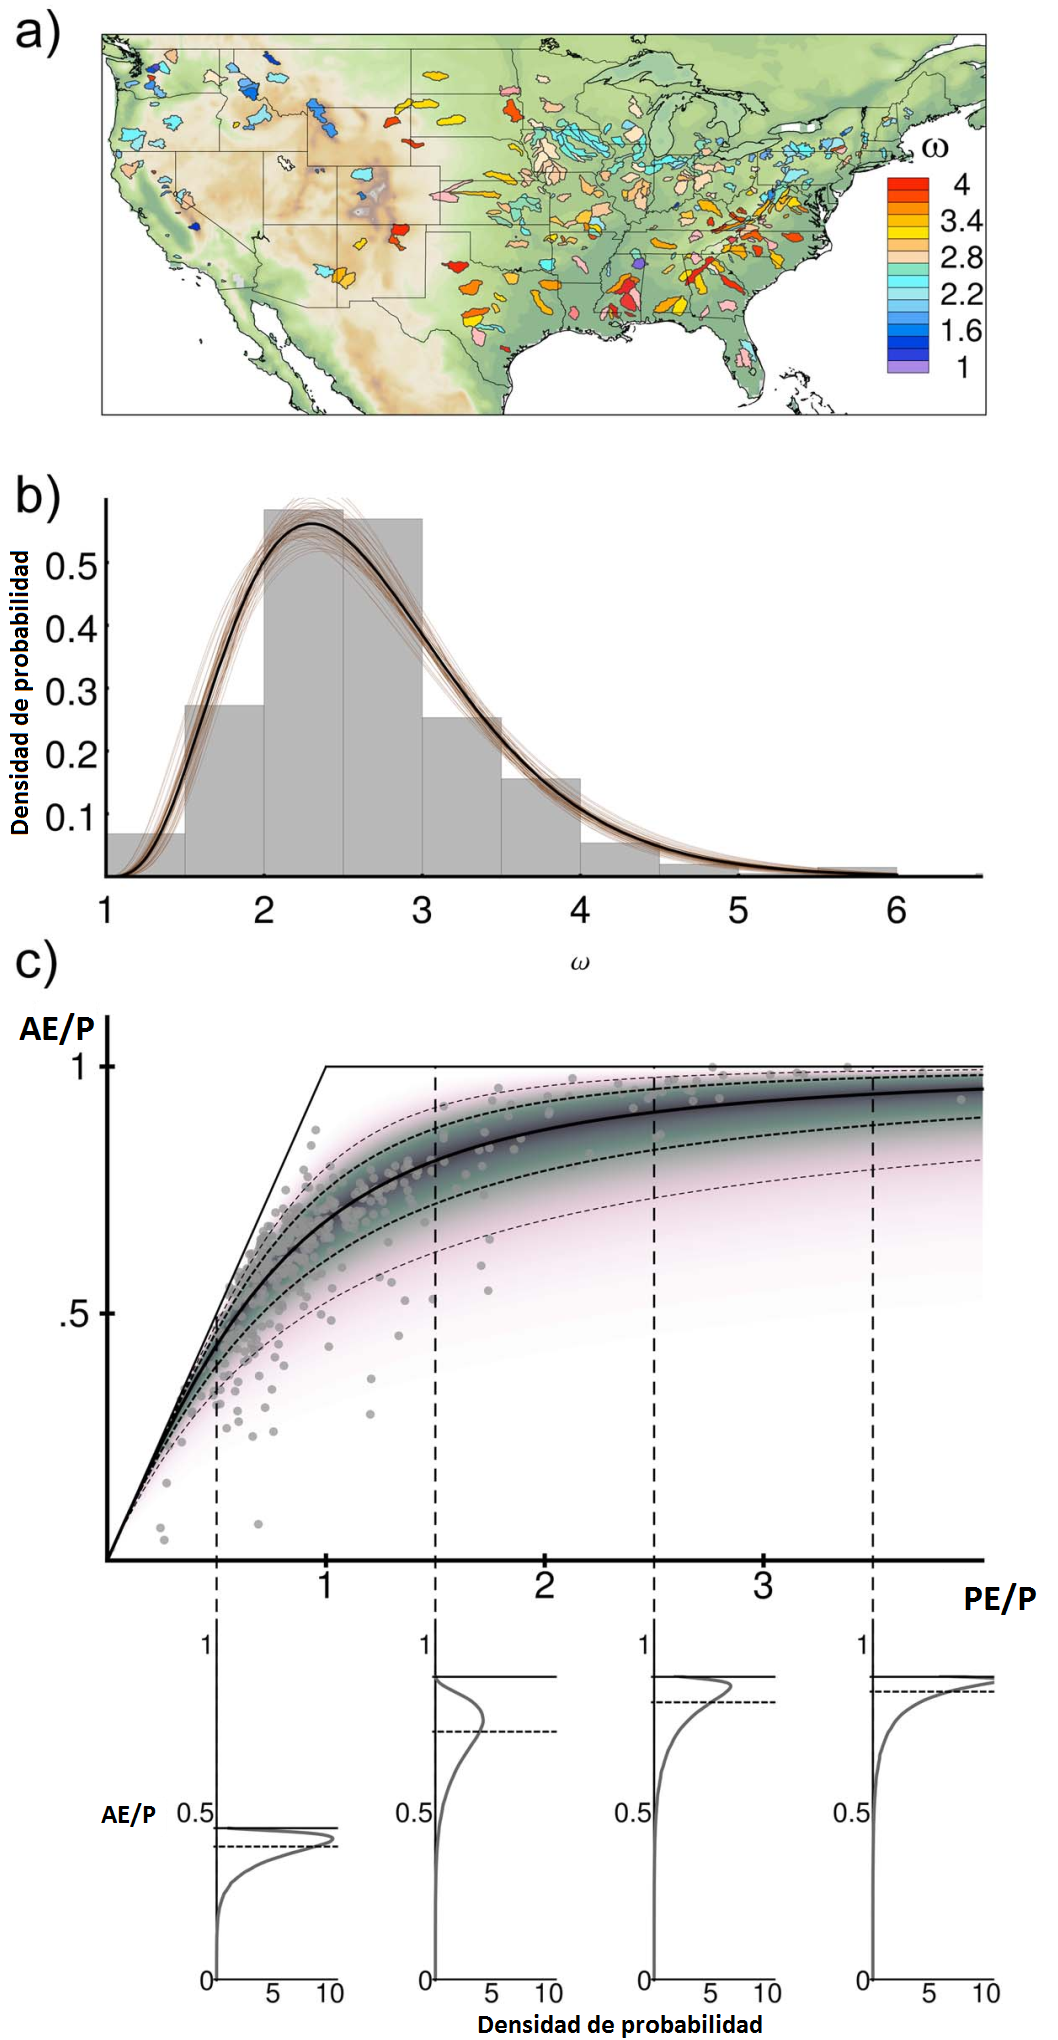
\includegraphics[scale=0.3]{Images/Greve03.png}
	\caption{a) Valor de $\omega$ para las 411 cuencas del MOPEX. b) Histograma de $\omega$ (barra gris) en conjunto con la distribución gamma ajustada (linea negra) y una muestra (bootstrapped) de distribuciones (lineas marrones). c) El enfoque de Budyko probabilístico estimado para las 411 cuencas. La distribución gamma es ajustada y utilizada para calcular la distribución de Budyko y las distribuciones de probabilidad condicionales para $PE/P = 0.5, 1.5, 2.5, 3.5$ (abajo). Las cuencas se muestran como puntos en gris.}
	{\raggedright FUENTE: \citet{Greve2015}. \par}
	\label{fig:Greve03}
\end{figure}
\clearpage

La curva media del Budyko probabilístico ($\omega = 2.56$) resulto ser bastante cercano a su valor original ($\omega = 2.6$). Además, se puede asumir que esta distribución de $\omega$ puede ser valida para todo tipo de condiciones climáticas debido a la propia naturaleza de $\omega$, la cual es independiente a $PE/P$. La distribución de Budyko obtenida se muestra en la Figura \ref{fig:Greve03}c en conjunto con las cuencas (en el espacio Budyko) del MOPEX.

\begin{figure}[ht]
\centering
	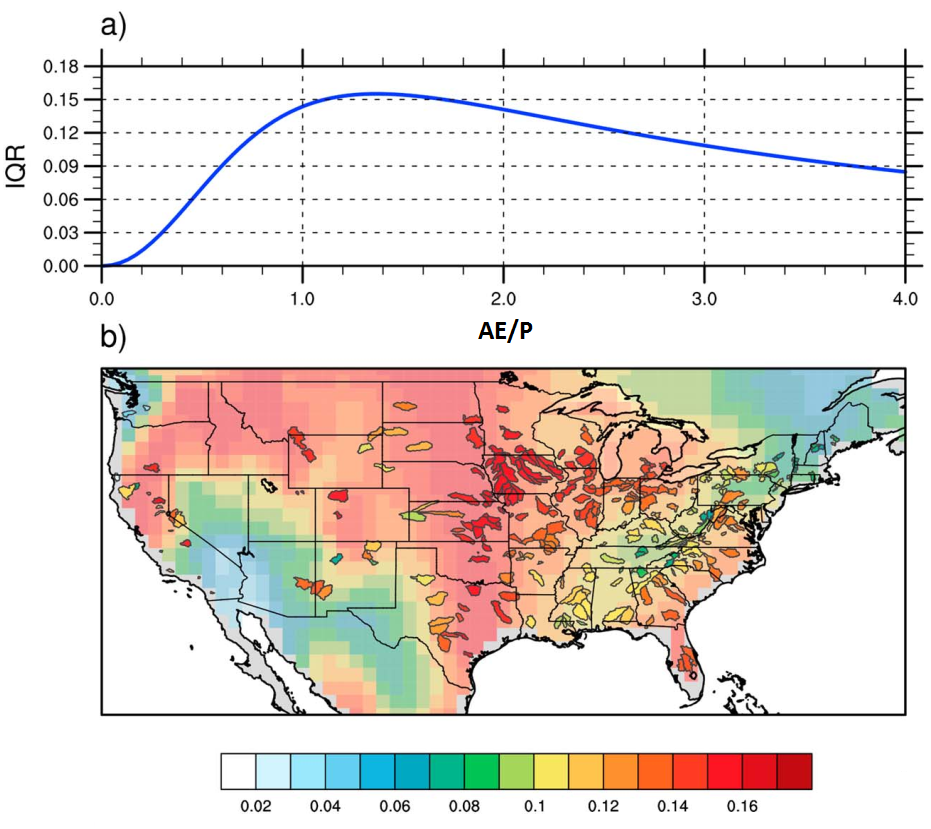
\includegraphics[scale=0.55]{Images/Greve04.png}
	\caption{Predictibilidad de $AE/P$. a) El rango intercuantil de $AE/P$ estimado de las distribuciones de Budyko que se muestra en la Figura \ref{fig:Greve03} condicionado a $PE/P$. b) El rango intercuantil condicional a $PE/P$ para cada una de las cuencas del MOPEX.}
	Fuente: \citet{Greve2015}.
	\label{fig:Greve04}
\end{figure}

La predictibilidad (inferencia) de $AE/P$ estimada por el Budyko probabilístico esta controlada por la distribución de $\omega$ (es decir, todas las variables que compacta este parámetro) y $PE/P$. Para determinar la incertidumbre asociado a $AE/P$, se hizo uso del rango intercuartil (IQR), una medida de dispersión, la cual es mostrada en la Figura \ref{fig:Greve04} en función de $PE/P$. Lo cual revelo que existe menores valores de IQR para condiciones muy húmedas (valores bajos de $PE/P$), llegando a su máximo valor en $PE/P = 1.4$. Entonces, bajo condiciones secas IQR permanece relativamente alto, pero disminuye lentamente al aumentar mas las condiciones secas. Esto sugeriría que existe mayor incertidumbre en las regiones climáticas de transición, lo que indica una menor predictibilidad de la disponibilidad de agua en comparación con las regiones húmedas o secas.

De igual manera, se cuantifico la incertidumbre de la predictibilidad de $AE/P$ en las cuencas del MOPEX, y su incertidumbre asociada por IQR. Se encontró mayor incertidumbre y, por ende, una baja predictibilidad para muchas cuencas en el oeste medio y montañas Rocky. La predictibilidad es ligeramente mejor para las cuencas del sudeste y noreste, incluidas algunas cuencas de los Apalaches. Las cuencas húmedas en el extremo noroeste revelaron mayor predictibilidad.

El otro caso de estudio de \citet{Singh2015} fue realizado con el objetivo de determinar la vulnerabilidad de los disponibilidad del agua en la India debido al cambio climático. Esto utilizando el enfoque “bottom-up" en conjunto con el Budyko probabilístico (también con la Ecuación \ref{equ:fuEqu} de \citet{Fu1981}). \citet{Singh2015} hizo uso de datos grillados de $T$, $P$ y $AE$, donde este ultimo fue proveniente de datos de percepción remota \citet{zhang2016review}, y su análisis fue a escala de distritos. La metodología empleada puede dividirse en tres principales pasos (Figura \ref{fig:Singh2015}): i) identificación de espacios climáticos vulnerables, ii) valores de $AE$ en función del paso i), y iii) vulnerabilidad y umbrales de cambio. 

\begin{figure}[ht!]
	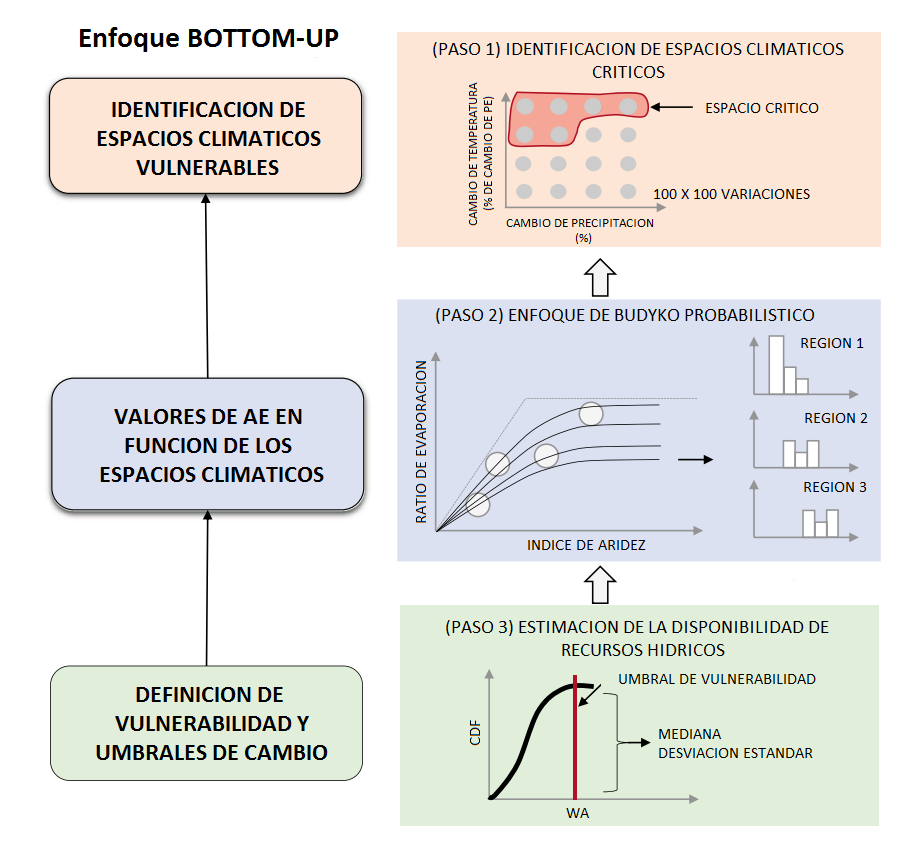
\includegraphics[scale=0.63]{Images/Singh2015.png}
	\centering
	\caption{Aplicación del enfoque “bottom-up" (en base a espacios climáticos) para evaluar la disponibilidad de los RH en la India. Selección de los espacios climáticos (paso 1), aplicación del Budyko probabilístico (paso 2) y estimación de la disponibilidad de los RH (paso 3).}
	{\raggedright FUENTE: \citet{Singh2015}. \par}

	\label{fig:Singh2015}
\end{figure}

En primer lugar, se determino los espacios climáticos (100 $\times$ 100, 1000 en total) de posibles variaciones futuras de las variables $P$ y $PE$ (en función de $T$). Para cada uno de estos escenarios se aplico el Budyko probabilístico para obtener proyecciones de $AE/P$. Lo que permitió no solo estimar la disponibilidad del agua, si no también la incertidumbre asociada (definición del método). Finalmente, se identifico umbrales de cambio critico donde se presento un decrecimiento de la disponibilidad de agua (aumento de la vulnerabilidad). Una diferencia principal al de la versión original de \citet{Greve2015}, fue que \citet{Singh2015} no ajusto una distribución teórica (no asunción de alguna forma particular), sino, solo utilizo la distribución empírica de $\omega$, la cual fue obtenida (calibrada) a escala de distrito y agrupada en seis regiones homogéneas. \citet{Singh2015} menciona que de esta manera no se pierde ninguna información de los datos y que a la vez se mantiene los supuestos sobre límites de incertidumbre de las estimaciones a un mínimo. Por lo tanto, se obtuvo seis distribuciones empíricas de $\omega$ en toda la India, las cuales fueron validadas a escala regional (en las seis) y nacional.

Los resultados demostraron que la variación del Budyko probabilístico de \citet{Singh2015} fue aceptable ya que se alcanzaron errores de hasta 18\% en la validación cruzada. Adicionalmente, mediante una variación de -50\% a 80\%, y de 0\% a 20\% en $P$ y $PET$ (en función de $T$) respectivamente se logro estimar la vulnerabilidad e incertidumbre asociada (visto como IQR) a escala de la India. Estos fueron comparados con las salidas de GCMs, demostrando no solo la capacidad del Budyko probabilístico, sino también del enfoque “bottom-up". De esto, se encontró que el cambio en $P$ tiene un control mucho mas fuerte sobre el valor medio del índice de vulnerabilidad que el cambio de $T$ (Figura \ref{fig:Singh02}). Los resultados también revelaron que las regiones que experimentan tendencias hacia condiciones secas tienen menores rangos de incertidumbre y viceversa en la escala de toda India, lo que se refleja en los valores más bajos de IQR en comparación con lo observado en las regiones que experimentan tendencias a ser mas húmedos.

Este mismo análisis se efectuó a escala de distrito, pero con la finalidad de identificar umbrales de cambio para un nivel de vulnerabilidad. La Figura \ref{fig:Singh02} muestra los cambios de $P$ que llevarían a una reducción del 25\% en la disponibilidad de los recursos hídricos para un nivel de cambio $PET$ (10\%). Esto fue posible al hacer uso de las distribuciones regionales de $\omega$. Resalta que el sur de la India es mas vulnerable a un decrecimiento de $P$, ya que una reducción de $10$ en $P$ conllevaría a un aumento de la vulnerabilidad de los recursos hídricos en 25\%. Similar a lo anterior, otros escenarios también puede ser factibles. 


\begin{sidewaysfigure}
	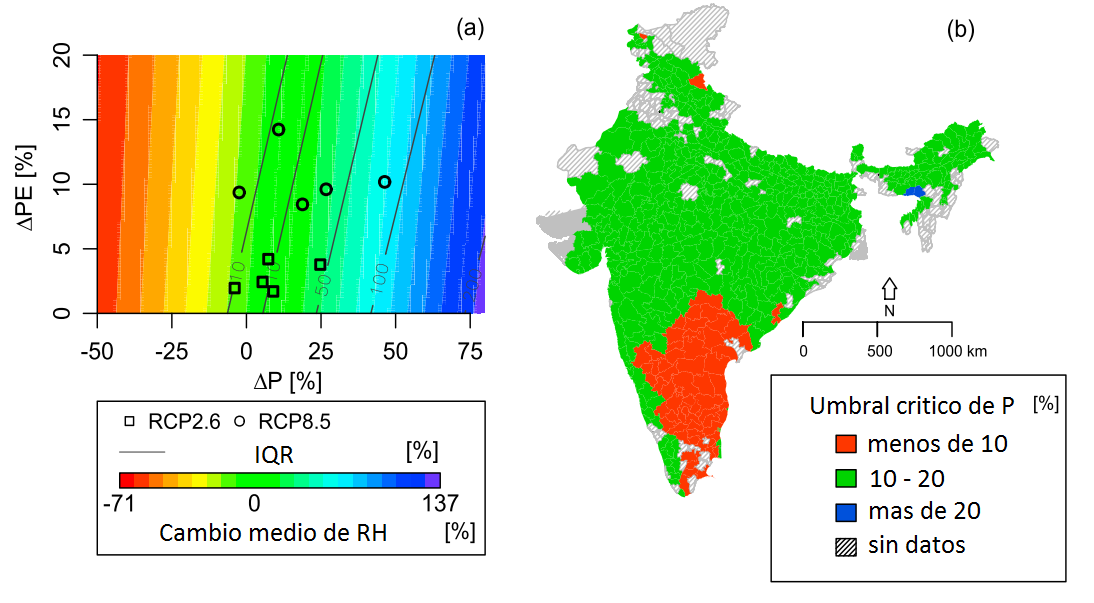
\includegraphics[scale=0.75]{Images/Singh02.png}
	\centering
	\caption{a) Vulnerabilidad de los RH a escala de la India estimada en función del cambio de precipitación ($\Delta P$) y evapotranspiración potencial ($\Delta PE$). Colores y lineas grises representan la mediana y el IQR del índice de vulnerabilidad. respectivamente. Adicionalmente se muestra (puntos y cuadrados) las proyecciones de $P$ y $PE$ de los modelos de cambio climático (CMIP-5). b) Variación espacial del cambio critico de $P$ que resulta en una reducción de 25\% de la disponibilidad RH en la India.}
	{\raggedright FUENTE: \citet{Singh2015}. \par}
	\label{fig:Singh02}
	
	\thisfloatpagestyle{empty}
\end{sidewaysfigure}



\clearpage
\vspace*{0.5mm}
\section{MATERIALES Y METODOLOGÍA}

\subsection{Materiales}

\subsubsection{Datos}

\begin{itemize}
  
  \item Datos de precipitación ($P$) y temperatura ($T$; máxima y mínima, $Tx$ y $Tn$ respectivamente).
  
  \item Datos de evapotranspiración actual ($AE$) basada en percepción remota.
  
  \item Datos de caudales ($Q$) disponibles a nivel nacional.

\end{itemize}

\subsubsection{Equipos}

\begin{itemize}
  \item 01 Ordenador personal - Lenovo ThinkPad T580.
  \item 01 Impresora.
\end{itemize}

\subsubsection{Programas de computo}

\begin{itemize}
  \item \LaTeX\  2018 - \url{https://www.overleaf.com}.
  \item Python 3.6.x - \url{https://github.com/adrHuerta/prob_Budyko}.
\end{itemize}

\subsection{Metodología}

\subsubsection{Recopilación de datos y materiales}

\paragraph{Precipitación y temperatura}\mbox{}

Debido al ámbito de estudio, se requiere información a escala de todo el territorio nacional. Por lo tanto se hizo uso de información grillada de $P$ y $T$ diaria del Servicio Nacional de Meteorología e Hidrología del Perú (SENAMHI), el producto de Datos Interpolados peruanos de las observaciones climatológicas e hidrológicas del SENAMHI (PISCO). De entre todas los datos grillados disponibles a escala nacional y global, PISCO representa la mayor asimilación de estaciones convencionales, y hace uso de otras fuentes de información para estimar los valores de precipitación y temperatura, adicionalmente, presenta un rango temporal adecuado para la investigación. El producto PISCO se divide en:

\begin{itemize}
	\item PISCO precipitación (PISCOp 2.1): PISCOp 2.1 es un producto combinado de tres fuentes principales \citep{Aybar2019}: observaciones de $P$ con control de calidad y completadas; satélite TRMM 2A25 \citep{iguchi2000rain} y datos grillados del CHIRP \citep{funk2015climate}. El marco metodológico comienza con una corrección climatológica mensual de CHIRP que se realiza mediante el uso de TRMM y valores observados. Usando el CHIRP corregido, se fusionó la $P$ a escala diaria y mensual usando regresión kriging (RK) y regresión de la distancia inversa ponderada (RIDW) respectivamente. Finalmente, se agregó un factor de corrección mensual con dos propósitos: proporcionar una mayor consistencia espacial a las predicciones diarias y garantizar que la agregación mensual del producto diario coincida con el producto mensual en cada punto de la cuadrícula. La validación independiente y la evaluación del balance hídrico demuestran que las estimaciones de $P$ son aceptables y muestran el rendimiento más alto para la costa del Pacífico y la zona occidental de los Andes.

\clearpage
	
	\item PISCO temperatura (PISCOt 1.1): PISCOt 1.1 es una base que incluye $Tn$ y $Tx$ \citep{Huerta2019}. Se basa en observaciones de $Tn$ y $Tx$ con control de calidad, completadas y homogeneizadas; temperatura superficial del suelo del satélite MODIS \citep{jin2010land}; y predictores topográficos como latitud, longitud, elevación y el índice de disección topográfica. La generación implica la estimación de climatologías mensuales usando RK ponderado y la estimación de anomalías mensuales y diarias usando regresión splines (RP). Los dos productos se suman y se obtiene el producto final. La validación cruzada de PISCOt 1.1 en el sur de los Andes muestra errores absolutos medios bajos (MAE) (0-0.5$^{\circ}$C) y pequeños sesgos que están cerca de cero para $Tx$, pero un MAE más alto (hasta 3$^{\circ}$C) y altos sesgos positivos y negativos (-3 a + 3$^{\circ}$C) para $Tn$.
	
\end{itemize}

Ambos productos se encuentran a una resolución espacial de 0.1$^{\circ}$ y temporalmente desde 1981-2016 (Figura \ref{fig:00_PISCOproducts}). La información fue obtenida a través del repositorio IRI/LDO Climate Data Library - \url{https://bit.ly/2kIVjPx}.

\vspace{1cm} %just for vertical space
\begin{figure}[ht]
	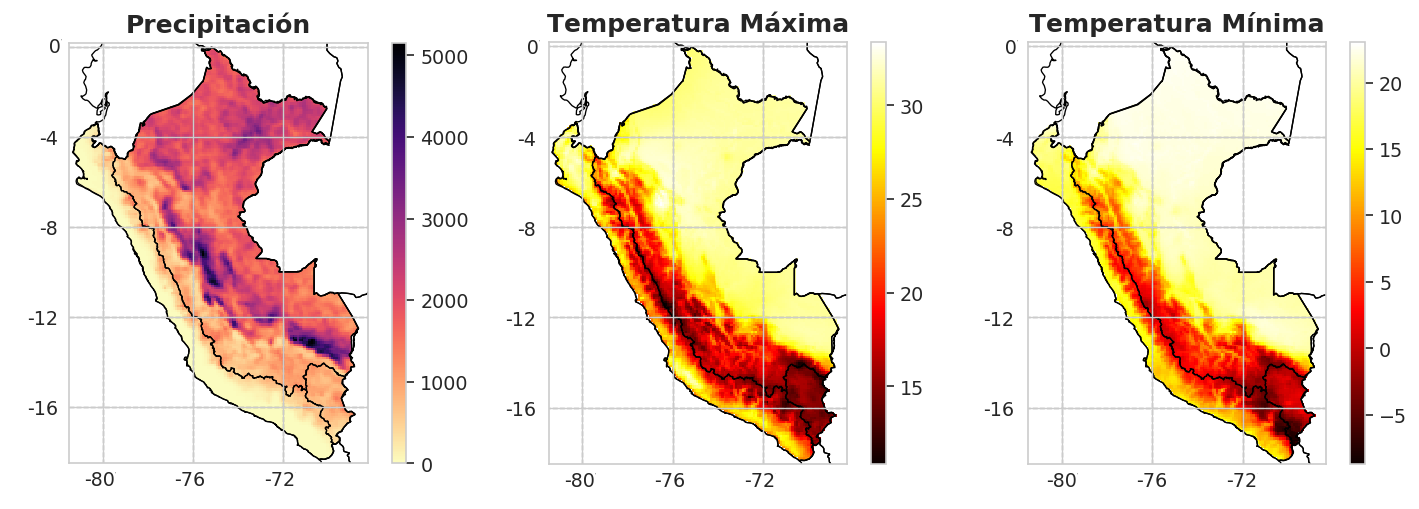
\includegraphics[width=16cm]{Images/00_PISCOproducts.png}
	\centering
	\caption{Producto PISCO de $P$ (mm) y de $Tx$ y $Tn$ ($^{\circ}$C). Valor total y promedio (respectivamente) para el año 2000.}
	\label{fig:00_PISCOproducts}
\end{figure}

\clearpage

\paragraph{Evapotranspiración actual}\mbox{}

Para la metodología propuesta se hace indispensable contar con datos de $AE$, sin embargo, no se cuenta con información observada en Perú. Por lo que se hace necesario usar productos grillados globales de $AE$, los cuales provienen de datos de percepción remota, satélite y reanalisis. Debido a que no existe un producto considerado el mejor a nivel del territorio nacional, se hace una selección y/o validación de los productos disponibles en este estudio, para posteriormente usar el de mejor rendimiento y/o que presente menor error. Los datos de $AE$ evaluados en esta tesis fueron: GLEAM, MODIS16, SSEBop, TerraClimate y Zhang. La Tabla \ref{tab:ETproducts} y Anexo 1 resume las características de los productos.

\begin{itemize}
	\item GLEAM: El Modelo Global de Evaporación Continental de Amsterdam (GLEAM) es un modelo basado en procesos, que describe empíricamente los procesos necesario para estimar $AE$ a partir de información satelital \citep{Martens2017}. El marco metodológico consiste en tres pasos: 1) interceptación de lluvia impulsada por observaciones de lluvia y vegetación; 2) evaporación potencial calculada usando la ecuación de PT e impulsada por observaciones satelitales; y 3) un factor de estrés que atenúa la evaporación potencial de acuerdo a una relación semi-empírica entre la vegetación de microondas y las observaciones de profundidad óptica (VOD) y las estimaciones de humedad del suelo de la raíz. %%% revisar GLEAM background
	
	\item MODIS16: El Proyecto Global de Evapotranspiración MODIS (MODIS16) estima la evapotranspiración terrestre utilizando datos de teledetección satelital. La $AE$ terrestre incluye la evaporación del agua y suelo húmedo, el agua de lluvia interceptada por el dosel y la transpiración a través de las estomas de las hojas y tallos de las plantas. Los datos de $AE$ se calculan de acuerdo a \citet{mu2013modis}, un algoritmo mejorado del propuesto por \citet{mu2007development}, y se basan en la ecuación de PM. Las mejoras incluyen: evaporación del suelo húmedo, $AE$ nocturno, calculo simplificado de la cobertura de la fracción vegetativa, flujo de calor del suelo, mejora de la estimación de conductancia estomática, resistencia aerodinámica y resistencia de la capa limite, separando las superficies de la cubierta seca y húmeda \citep{mu2013modis}.
	
	\item SSEBop: El Modelo Operativo de Balance de Energía de Superficie Simplificado (SSEBop) estima $AE$ en función de datos de temperatura del suelo (LST) y la evapotranspiración potencial ($PE$) de reanalisis, utilizando el método de balance de energía de superficie simplificado (SSEB) desarrollado por \citet{senay2007coupled,senay2011enhancing}. El SEB resuelve por cada píxel y para cada condición de cultivo de referencia la ecuación P-M estándar y se ajusta de acuerdo a LST a través de un enfoque de fracción $AE$, que explica la variabilidad espacial de la disponibilidad de agua y la salud de la vegetación en el paisaje \citep{savoca2013actual}. SSEBop utiliza condiciones de frontera estacionalmente dinámicas predefinidas que son exclusivas de cada píxel para los puntos de referencia ``caliente/seco" y ``frío/húmedo" según \citet{bastiaanssen2014earth} y \citet{allen2007satellite}.
	
	\item TerraClimate: TerraClimate es un conjunto de datos climáticos y balance hídrico climático para las superficies terrestres globales \citep{abatzoglou2018terraclimate}. TerraClimate utiliza interpolación asistida por el clima, combinando normales climatológicas de alta resolución espacial del conjunto de datos WorldClim \citep{fick2017worldclim}, con una resolución espacial más gruesa, pero datos que varían en el tiempo del CRU TS4.0 \citep{harris2014updated} y el reanalisis japonés JRA55 \citep{kobayashi2015jra}. TerraClimate también produce conjuntos de datos mensuales de balance de agua superficial utilizando un modelo de balance de agua que incorpora $PE$, $P$, $T$ y capacidad de agua extraíble de la planta interpolada. Para estimar $AE$ se utilizo el modelo de Thornthwaite-Mather \citep[T-M;][]{willmott1985climatology} modificado y datos extraíbles de capacidad de almacenamiento de agua del suelo en una cuadrícula de 0.5$^{\circ}$ de \citet{wang2016global}.
	
	\item Zhang: Es un producto de $AE$ que usa un algoritmo impulsado por datos de sensoramiento remoto y reanalisis \citep{zhang2010continuous}. El algoritmo cuantifica la transpiración del dosel y la evaporación del suelo utilizando un enfoque P-M modificado con una conductancia del dosel específica del bioma determinado a partir de la diferencia del índice de vegetación normalizada (NDVI) y cuantifica la evaporación de aguas abiertas utilizando un enfoque de P-T. Estos algoritmos se aplicaron globalmente utilizando datos de radiómetro de muy alta resolución AVHRR \citep{tucker2005extended}, datos meteorológicos diarios de superficie del NCEP/NCAR (NNR) \citep{kistler2001ncep} y entradas de radiación solar de la NASA/ GEWEX \citep{pinker1992modeling}. En \citet{zhang2015vegetation}, se realizo una serie de mejoras en el algoritmo para tener en cuenta la influencia de la velocidad del viento y las concentraciones de CO$_{2}$ atmosférico en los respectivos términos de conductancia aerodinámica y conductancia estomática del dosel, y en los cálculos de $AE$ resultantes.
	
	\item MEAN: Es el producto de $AE$ que se obtiene al promediar los anteriores bases de datos. MEAN se calcula a escala anual y se realizo con el motivo de reducir la incertidumbre de los diferentes productos de $AE$. 
	
\end{itemize}

\paragraph{Caudales}\mbox{}

Para la investigación se obtuvo información de caudales que se encuentran en la salida de flujo principal de la cuenca. Se utilizaron alrededor de 13 estaciones hidrológicas del trabajo de \citet{Aybar2019}, las cuales fueron provistas por SENAMHI y del Observatorio de Investigación Ambiental (SO-HYBAM). La información se encuentra a escala temporal mensual en el periodo de 1980 al 2016. Se debe mencionar que la información presenta un control de calidad riguroso y no esta completado. Las estaciones a usar fueron (Figura \ref{fig:00_all_basins}): Ardilla (ARD), Borja (BRJ), Bella Unión (BUN), Conta (CNT), Chazuta (CZT), Huatiapa (HTP), La Tranca (LTC), Letrayoc (LTY), Puchaca (PCH), Pucallpa (PCP), Puente Ramis (RMS), Requena (RQN) y Yanapampa (YNP).

\clearpage
\begin{sidewaystable}
\caption{\label{tab:ETproducts} Características de los diferentes productos globales de $AE$ basados en percepción remota utilizados.}
\centering
\begin{tabular}{llllllll}
\hline 
Producto     & Cobertura & Cobertura & Resolución & Resolución & Enfoque de                & Datos de   & Referencia      \\
             & temporal  & espacial  & temporal   & espacial   & estimación                & entrada    &                 \\   \hline
GLEAM        & 1980-2016 & Global    & Diario     & 0.25 x     & Ecuación P-T              & AMSR-E     & \citet{Martens2017}     \\
v.3.3a      &           &           &            & 0.25       & Factor de estrés de suelo & LPRM       &                 \\
             &           &           &            &            &                           & TRMM       &                 \\
MODIS16      & 2000-2014 & Global    & Mensual    & 0.0083 x   & Ecuación PM              & MODIS      & \citet{mu2013modis}         \\
v.105         &           &           &            & 0.0083     & Modelo de conductancia    &            &                 \\
             &           &           &            &            & de superficie             &            &                 \\
SSEBop       & 2003-2017 & Global    & Mensual    & 0.0096 x   & Ecuación PM              & MODIS      & \citet{senay2011enhancing}      \\
v4.0         &           &           &            & 0.0096     & Fracciones ET de LST      &            &                 \\
TerraClimate & 1958-2015 & Global    & Mensual    & 0.04 x     & Balance hídrico del suelo & WorldClim  & \citet{abatzoglou2018terraclimate} \\
             &           &           &            & 0.04       & unidimensional            & CRU        &                 \\
             &           &           &            &            &                           & JRA55      &                 \\
P-LSH        & 1981-2013 & Global    & Mensual    & 0.083 x    & Ecuación PM              & AVHRR      & \citet{zhang2015vegetation}      \\
             &           &           &            & 0.083      & Balance hídrico del suelo & NCEP/NCAR  &                 \\
             &           &           &            &            &                           & NASA/GEWEX &                 \\
PROMEDIO         & 2003-2013 & Global    & Anual      & 0.01 x     & -                         & -          & Tesis actual    \\
             &           &           &            & 0.01       & -                         & -          &                  \\ \hline 
\end{tabular}

\thisfloatpagestyle{empty}
\end{sidewaystable}
\clearpage
\begin{figure}[ht!]
	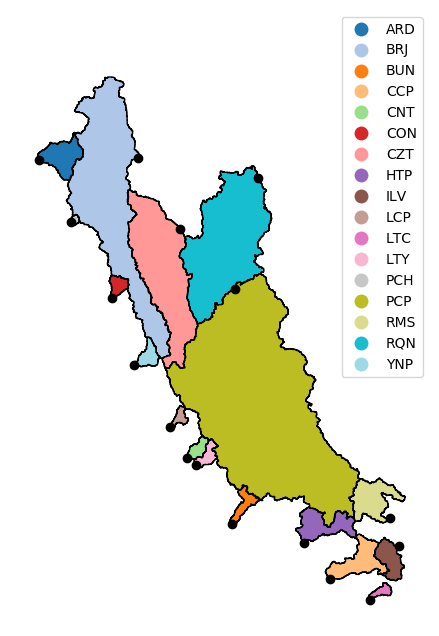
\includegraphics[scale=1.1]{Images/00_all_basins.png}
	\centering
	\caption{Potenciales cuencas hidrográficas a usar para la evaluación de $AE$.}
	\label{fig:00_all_basins}
\end{figure}
\clearpage

\subsubsection{Esquema metodológico}

La investigación se inspira en los trabajos de \citet{Singh2015} y \citet{Weerasinghe2019discuss}, y se divide en tres principales pasos: 1) Selección del mejor producto de evapotranspiración actual basado en percepción remota; 2) Budyko probabilístico; y 3) Estimación Vulnerabilidad de la disponibilidad del RH en el futuro. Una visualización esquemática de lo anterior se encuentra en la Figura \ref{fig:workflow}, donde se muestra el proceso completo para la realización de la investigación. En las secciones posteriores se detalla los pasos de la Figura \ref{fig:workflow}.

\vspace{.25cm}
\begin{figure}[ht]
	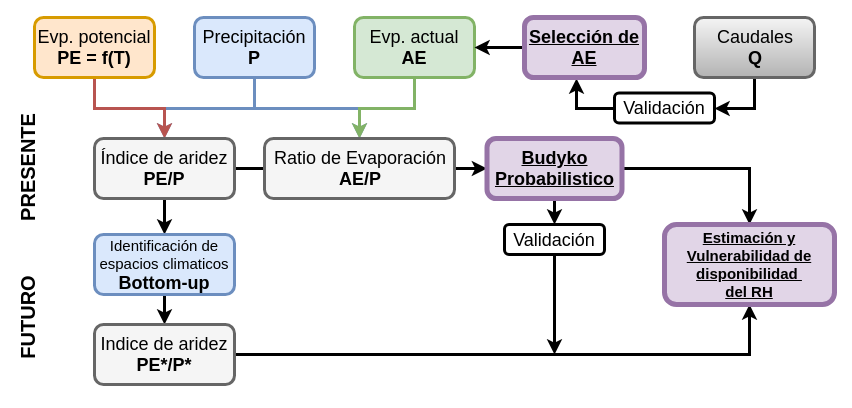
\includegraphics[scale=0.49]{Images/workflow.png}
	\centering
	\caption{Esquema metodológico de la investigación.}
	\label{fig:workflow}
\end{figure}

Toda la información ($P$, $T$, $PE$, $AE$ y $Q$) fue analizada y validada a escala climática, es decir a nivel de promedio anual y a escala espacial de cuenca hidrográfica. Solo la información de $PE$ (en función de $T$) se calculo a nivel diario y acumulado para obtener valores anuales, y posteriormente, sus climatologías. Los datos grillados se interpolaron (nearest neighbor) a una escala de 0.01$^{\circ}$ con la finalidad de facilitar su inter-comparación. El periodo climático en este estudio se establece entre los años 2000 y 2014, esto por las diferentes razones:

\begin{itemize}

	\item Existe mayor acople (datos) para toda la información a usar ($P$, $T$, $PE$, $AE$ y $Q$. Esto principalmente para los productos de $AE$.
	
	\item La $P$ y $T$ provenientes del producto PISCO en el periodo designado presentan la menor cantidad de información completada, haciendo que exista menor incertidumbre en el grillado de esas variables \citep{Huerta2019, Aybar2019}.
	
	\item Los datos de $Q$ históricos presentan posiblemente grandes incertidumbres en sus consistencia, ya que existe poca o nula metadata que refleje su calculo (curvas de duración, aforo, etc.). Por lo que es mas fiable usar datos de los últimos años.
	
	\item Es posible encontrar tendencias naturales y/o artificiales en datos pasados, haciendo que la validación y/o análisis climático que se realiza en este investigación tenga un enfoque no-estacionario (quitar tendencias). Sin embargo, esto es prácticamente imposible de realizar debido a la escasa información de $Q$, y baja disponibilidad de productos de $AE$ antes del 2000.
	
\end{itemize}

En primer lugar (Paso 1, Figura \ref{fig:workflow}), se hace una selección del mejor producto de $AE$ considerando la información de $Q$. Una vez seleccionado $AE$, se procede a estimar $PE$, el cual es calculado mediante $Tx$, $Tn$ y la radiación extraterrestrial ($R_{a}$) usando la ecuación de \citet{Hargreaves1985}:

\begin{equation}
PE = 0.0023R_{a}\left ( \frac{T_{x}+T_{n}}{2} \right )\left ( T_{x}+T_{n} \right )^{0.5}
\end{equation}

Calculado $P$, $PE$ y $AE$ a escala climática, se procede a la extracción del valor areal correspondiente a las diferentes cuencas de las Unidades Hidrográficas (UH) de la Autoridad Nacional del Agua (ANA, Figura \ref{fig:00_vertientes}). Por cada UH se obtiene el valor promedio que corresponde a toda la cantidad de píxeles o grillas que se encuentren en su interior. Una vez lo anterior, se procede al análisis de Budyko probabilístico (Paso 2, Figura \ref{fig:workflow}). En aquellas UH que no cumplan la restricción física de las leyes de suministro de humedad atmosférica ($AE < PE$, es decir, valores que se encuentran fuera de las límites de energía y agua en la curva de Budyko) serán removidas del análisis. Posteriormente, se calibra/valida en el tiempo presente (con las climatologías); y finalmente (Paso 3, Figura \ref{fig:workflow}) los valores futuros de $PE$ y $AE$ por diferentes combinaciones de $P$ y $T$ (espacios climáticos), aplicándose nuevamente la formulación del Budyko probabilístico para obtener proyecciones del ratio de evaporación. De esta manera, se estimo la disponibilidad de agua y su incertidumbre asociada con la información generada.

Desde la perspectiva de \citet{Singh2015}, partiendo ya con un producto de $AE$ seleccionado, se tiene como primer paso la identificación de los espacios climáticos, seguido por la aplicación del enfoque probabilístico y finalmente la estimación de la disponibilidad de los RH. Estos pasos se encuentran descritos en las secciones de Revisión de literatura. La Figura \ref{fig:Singh2015} presenta el orden según \citet{Singh2015}, así como también diagramas representativos del mismo.

\vspace{.25cm}
\begin{figure}[htb!]
\centering
	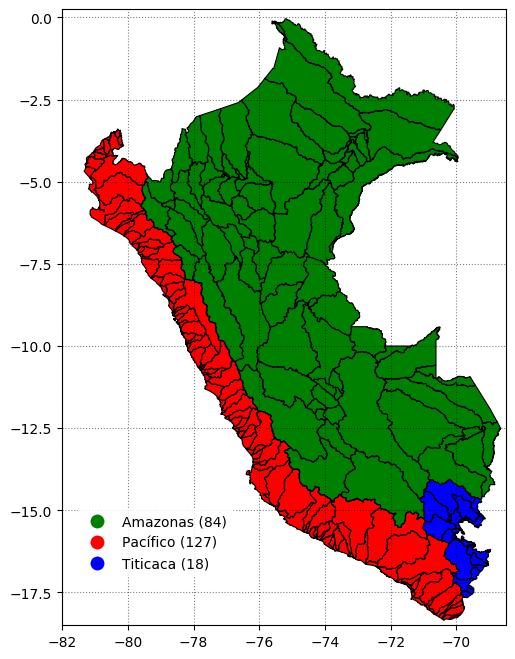
\includegraphics[scale=1]{Images/00_vertientes.png}
	\caption{Vertientes y unidades hidrográficas (número) usadas en el estudio.}
	\label{fig:00_vertientes}
\end{figure}

\subsubsection{Selección de producto de evapotranspiración actual}

Debido a la limitada o nula disponibilidad de observaciones directas de $AE$ en Perú, se hace uso de datos globales de $AE$ provenientes de fuentes de percepción remota, satélite y/o reanálisis. El uso de $AE$ independiente también debe satisfacer el balance de agua y energía para un volumen control \citep{Singh2015}.

Para establecer correctamente que producto de $AE$ global a usar se hace un ranqueo y posterior selección, esto a través de una validación con datos de $AE$ observado. El $AE$ observado se infiere de estimaciones de:

\begin{itemize}

	\item Balance Hídrico: El balance hídrico a largo plazo supone un cambio insignificante en el almacenamiento (discutido el ítem 2.3), por lo tanto, cambiando el orden de la Ecuación \ref{equ:WB}:
	
	\begin{equation}
    AE = P - Q
    \label{equ:bheq}
    \end{equation}

	\item Budyko: La ecuación de Budyko divide $P$ en $AE$ y $Q$ al describir la relación climática entre $AE$ y el balance de agua y energía (discutido en el ítem 2.3). Multiplicando por P la Ecuación \ref{equ:fuEqu}
    \begin{equation}
    AE = P + PE - P\left (1 + \left ( \frac{PE}{P} \right )^{2.6}  \right )^{1/2.6}
    \end{equation}
	
\end{itemize}


\paragraph{Validación}\mbox{}

Las métricas para caracterizar los productos de $AE$ y determinar el ranqueo fueron las siguientes:

\begin{itemize}

	\item Similaridad (Td): La métrica Td explica las diferencias tanto en el patrón espacial como en la amplitud entre un par de productos \citep{Tian2017}. Td vas desde 0 (sin similiridad) a 1 (similaridad perfecta) y se calcula como:
	
	\begin{equation}
    Td = [(1 + R) / 2]*[1 - MSE/bias]
    \end{equation}
    
    donde, R es la correlación de Pearson, MSE el error medio, y bias el error simple.
    

	\item Correlación de Spearman (Rs): Similar en interpretación pero mas robusta que R, Rs refleja la relación lineal (y no lineal) entre dos observaciones. Mientras Rs este próximo a 1, existe una solida relación entre ambas variables.
	
	\item Error cuadrático medio (RMSE): Es la raíz cuadrada de MSE y se calcula de la siguiente manera:
	
    \begin{equation}
        RMSE = \sqrt{MSE} = \sqrt{\frac{1}{N} \sum_{i=1}^{N}(AE_{producto}-AE_{inferido})^{2}}
    \end{equation}
    
    donde, N es el numero de pares de datos.
    
	\item Error simple (Bias): Es la diferencia entre el valor observado y del modelo. Para este estudio seria:
	
    \begin{equation}
        bias = AE_{producto}-AE_{inferido}
    \end{equation}
	
\end{itemize}

Solo Td se utilizo para hacer hincapié en la similaridad de los diferentes productos de $AE$ basado en percepción remota. El resto de métricas se calcularon usando todas las potenciales cuencas de evaluación de $Q$. Solo el bias se calculo para cada cuenca de evaluación y producto de $AE$. Finalmente, se renquea y selecciona el mejor $AE$, para ser utilizado en los siguientes pasos.

\subsubsection{Budyko probabilístico}

Originalmente la curva de Budyko fue propuesta mediante una relación invariante en el espacio-tiempo \citep{Budyko1961,Pike1964}. Sin embargo, evidencia ha demostrado que las características de la cuenca y del clima afectan su posición en la curva. Por lo tanto, las diversas versiones paramétricas de la curva de Budyko tienen base determinista en su formulación \citep{Fu1981,Zhang2004,Zhang2008,Wang2014}. En este estudio se usa la ecuación de \citep{Fu1981} (Ecuación \ref{equ:fuEqu} y Figura \ref{fig:Greve01}), y esta estipula que las condiciones promedio climáticas a largo plazo mediante $PE/P$ es el factor primario que controla $AE/P$. El parámetro $\omega$ integra los efectos secundarios de la variabilidad climática y características biofísicas como el terreno, suelo, vegetación, etc. \citep{Gentine2012,Berghuijs2014,Greve2015}.

Recientemente, una extensión de la base determinista de Budyko ha sido desarrollado, re-formulándolo a un enfoque probabilístico \citep{Greve2015}. Basado en \citet{Greve2015}, es posible calibrar la ecuación de \cite{Fu1981} usando la información histórica disponible para obtener estimaciones óptimas de $\omega$ para un volumen de control (cuenca). Debido a la propia naturaleza de $\omega$ que cuenta con un error inherente (de los datos), los $\omega$ calibrados a nivel de UH son agrupados a macro-unidades de UH (vertientes hidrográficas) para obtener distintas distribuciones regionales de $\omega$ a nivel nacional. La Figura \ref{fig:Greve02}b muestra un ejemplo del Budyko probabilístico para diferentes tipos de distribución de $\omega$, otras, mayor detalle en \citet{Greve2015}. En este estudio no se asumirá alguna distribución teórica inicial del parámetro de la curva de Budyko, sino se usa directamente la distribución empírica de los datos, similar a \citet{Singh2015}. De esta manera no se pierde información valiosa de los datos y manteniendo los supuestos en los límites de incertidumbre de las proyecciones a un mínimo (Figura \ref{fig:Singh2015}).

\paragraph{Calibración}\mbox{}

La calibración del parámetro de $\omega$ se obtuvo mediante la minimización del RMSE entre el observado y estimado (por el Budyko). Similar técnica fue implementada en los trabajos en \citet{Zhang2004}, \citet{xiong2012appraisal}, y \citet{Singh2015}.

\clearpage %to avoid a title in the bottom of a page 
\paragraph{Validación cruzada}\mbox{}

Para este proceso, el valor del parámetro $\omega$ en cada UH fue agrupada a cada nivel macro de cuenca (vertiente hidrográfica), y sucesivamente a nivel nacional. Por lo tanto, las UH dentro de un determinado nivel macro compartirán el juego de parámetros $\omega$ lo que conlleva a la distribución empírica de $\omega$. Este proceso es repetido a nivel nacional compartiendo el juego de parámetros por cada UH. Entonces la validación cruzada es realizada de la siguiente manera:

\begin{itemize}
  \item Validación de $AE/P$: Se estima $AE/P$ usando el juego de parámetros $\omega$ a nivel de UH, macro (vertiente hidrográfica) y nacional, posteriormente se compara con los $AE/P$ utilizados. La métrica a utilizar para la comparación es el bias porcentual:
  
    \begin{equation}
    \%\ bias = \frac{Observado-Modelo}{Observado}*100
    \end{equation}
\end{itemize}


\subsubsection{Disponibilidad de los recursos hídricos debido al cambio climático}

Para evaluar la vulnerabilidad de la disponibilidad de los RH debido al cambio climático se utilizo el enfoque “bottom-up" (espacios climáticos), así como también se definió la vulnerabilidad.


\paragraph{Espacios climáticos}\mbox{}

Debido a la inherente incertidumbre de las proyecciones climáticas a tal punto que la dirección de cambio se vuelve incierta, principalmente para la disponibilidad de agua, se hace necesario usar nuevos enfoques de análisis tales como “bottom-up". Contrario al método “top-down“, en que usualmente un modelo hidrológico utiliza las proyecciones de cambio climático disponible para obtener cambios futuros de una variable determinada. Los planteamientos “bottom-up" enfatizan la identificación de rangos de variabilidad (vulnerabilidad) de la variable a estudiar y luego encuentra regiones en el espacio climático que probablemente causen la variabilidad.

En este estudio, se utilizo la perspectiva “bottom-up" para estimar un gran número de posibles escenarios climáticos para Perú que abarcan las proyecciones futuras de América del Sur. Se creará una matriz de 100*100 posibles escenarios, resultando en 10000 posibles combinaciones climáticas de $P$ y $PE$ (a través de $T$), representando así el índice de aridez $PE/P$ el cual será insertado en el Budyko probabilístico calibrado, obteniendo así, valores de $AE/P$ futuros (de cada espacio climático) necesarios para estimar la disponibilidad proyectada (Figura \ref{fig:Singh2015}).

\paragraph{Vulnerabilidad de la disponibilidad del RH}\mbox{}

El balance hídrico en una determinada cuenca puede ser expresada de acuerdo \citep{Singh2015}:

\begin{equation}
\frac{\partial S_{t}}{\partial t} = P_{t} + GW_{in,t} + Q_{in,t} - GW_{out,t} - Q_{out,t} - AE_{t} 
\end{equation}

Donde, $S$ es el almacenamiento hidrológicamente activo, $GW_{in}$ ($_{out}$) es la entrada (salida) de agua subterránea de la cuenca, $Q_{in}$ ($_{out}$) es la entrada (salida) de agua en la superficie de la cuenca en el tiempo $t$, y el resto de variables ya definidas anteriormente. Entonces la disponibilidad de agua es dado por:

\begin{equation}
WA_{t} =  GW_{in,t} + Q_{in,t} - GW_{out,t} - Q_{out,t}
\end{equation}

Donde, $WA$ representa la disponibilidad de $RH$ en el periodo $t$ representando la salida neta de agua de superficie y subterránea para una cuenca. Para escalas de tiempo anuales a decadales se puede asumir que el cambio neto en el almacenamiento hidrológicamente activo en una cuenca es cero. Por lo tanto, la disponibilidad de $RH$ puede ser simplificada como: 

\begin{equation}
WA_{t} = P_{t} - AE_{t}
\end{equation}

En este estudio para estimar la proyección de $WA$ es requerido estimar la proyección de $AE$ y $P$, entonces estas variables son asimiladas en la ecuación de Budyko probabilístico calibrado.

En conjunto con lo identificación de los espacios (escenarios) climáticos se estima $WA$ (a partir de la curva de Budyko) para cada combinación entre $PE/P$ proyectado. Con cada valor de $PE/P$ en una determinada UH se obtiene la distribución de probabilidad de $WA$ considerando el juego de parámetros $\omega$. Entonces la vulnerabilidad de la disponibilidad de agua debido al cambio climático es calculado basada en el cambio relativo de sus valores históricos:

\begin{equation}
VI = \frac{\Delta WA}{WA}100
\end{equation}

Donde $VI$ es el índice de vulnerabilidad, $WA$ es la disponibilidad de agua a largo plazo histórico definida anteriormente y $\Delta WA$ es el cambio de la disponibilidad de agua a largo plazo. Debido a la formulación de $VI$ para un rango de climas, es posible identificar umbrales de clima críticos para un nivel de vulnerabilidad elegido. Adicionalmente, es posible estimar la incertidumbre asociada a cada espacio climático (Figura \ref{fig:Singh2015}).

\clearpage
\vspace*{0.5mm}
\section{RESULTADOS Y DISCUSIONES}

Los resultados y discusiones se presentan teniendo en cuenta los objetivos específicos: i) Selección de productos globales de $AE$; ii) Aplicación del marco de Budyko probabilístico; y iii) Estimación la disponibilidad de RH e incertidumbre asociada frente al cambio climático.

\subsection{Selección de producto de evapotranspiración actual}

En la Figura \ref{fig:02_AEproducts} se aprecia la climatología anual de $AE$ para los diferentes productos globales de la Tabla \ref{tab:ETproducts}. Como primera aproximación, se evidencio una clara diferencia entre las mismas, principalmente en la vertiente de Pacifico, donde $AE$ tiende a cambiar abruptamente (Zhang y SSEBop). De igual manera en la vertiente del Amazonas se presenta altos contrastes, particularmente en la transición Andes-Amazonas (MODIS16, TerraClimate y SSEBop). 

\begin{sidewaysfigure}
	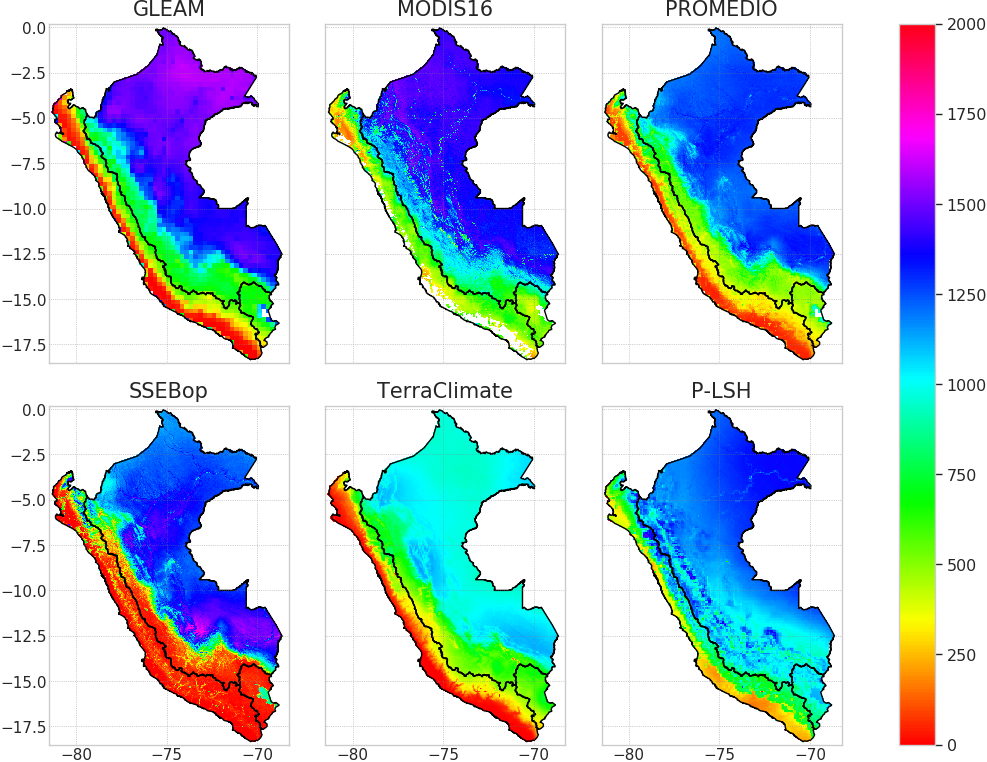
\includegraphics[scale=.8]{Images/02_AEproducts.png}
	\centering
	\caption{Climatología anual de $AE$ basados en percepción remota (2003-2013).}
	\label{fig:02_AEproducts}
\end{sidewaysfigure}


Para un mejor entendimiento de la similaridad entre los diferentes productos de $AE$, se hace uso de la matriz Td (Figura \ref{fig:03_Tindex_AEproducts}). La matriz Td muestra el calculo entre pares de productos de la métrica Td. Considerando esta matriz, todos los productos tiene una alta similaridad (Td $>$ 0.75), sin embargo hay algunos con mucho mas similitud entre si (próximos a 1). Entre los productos que difieren mas con el resto fueron MODIS16 y Zhang, y particularmente entre estas mismas se tiene el valor mas bajo de similitud lo cual se evidencia al visualizar sus valores de $AE$ en la Figura \ref{fig:02_AEproducts} (principalmente en la vertiente del Titicaca y en los Andes). Caso opuesto (Td próximo a 1) se tiene a GLEAM y MEAN, que se consideran como los de mayor similitud entre el resto, solo existe disparidad en la magnitud de $AE$ al sur de la vertiente Amazónica (Figura \ref{fig:02_AEproducts}). TerraClimate es también próximo a GLEAM y MEAN con una medida levemente menor de similiridad, a razón de mayor discrepancia en la transición Andes-Amazonia con los anteriores productos.

Por lo tanto se puede afirmar que GLEAM, TerraClimate y MEAN son los productos que tiene mayor similaridad, a diferencia de MODIS16 y ZHANG las cuales divergen mas. A pesar de la alta similitud, cada producto presenta ciertas particularidades. Por ejemplo MODIS16 no estima $AE$ en la parte costera de la vertiente del Pacífico, el algoritmo de MODIS16 no incluye áreas urbanas y áridas debido a que no hay la relación de fracción de radiación fotosintéticamente activa e índice de área foliar (FPAR/LAI) para este tipo de cobertura \citep{mu2013modis}. Por otro lado, GLEAM tiende a sobrestimar $AE$ cerca a la linea costera debido, a que por el tamaño de píxel (baja resolución), la fracción de tipo de suelo (en esas áreas) considera mayor cantidad de agua que tierra conllevando a una evaporación sin estrés resultando en valores muy altos \citep{Martens2017}. Lo anterior se evidencia en MEAN ya que al promediar tales valores, difieren mucho del resto de productos. Por otro lado, SSEBOp es el que tiene los valores mas bajos de AE, tanto así, que en los Andes llega a tener menos de 500mm, contrario al resto de productos alcanzando aproximadamente 1000mm.

\begin{figure}[htb]
	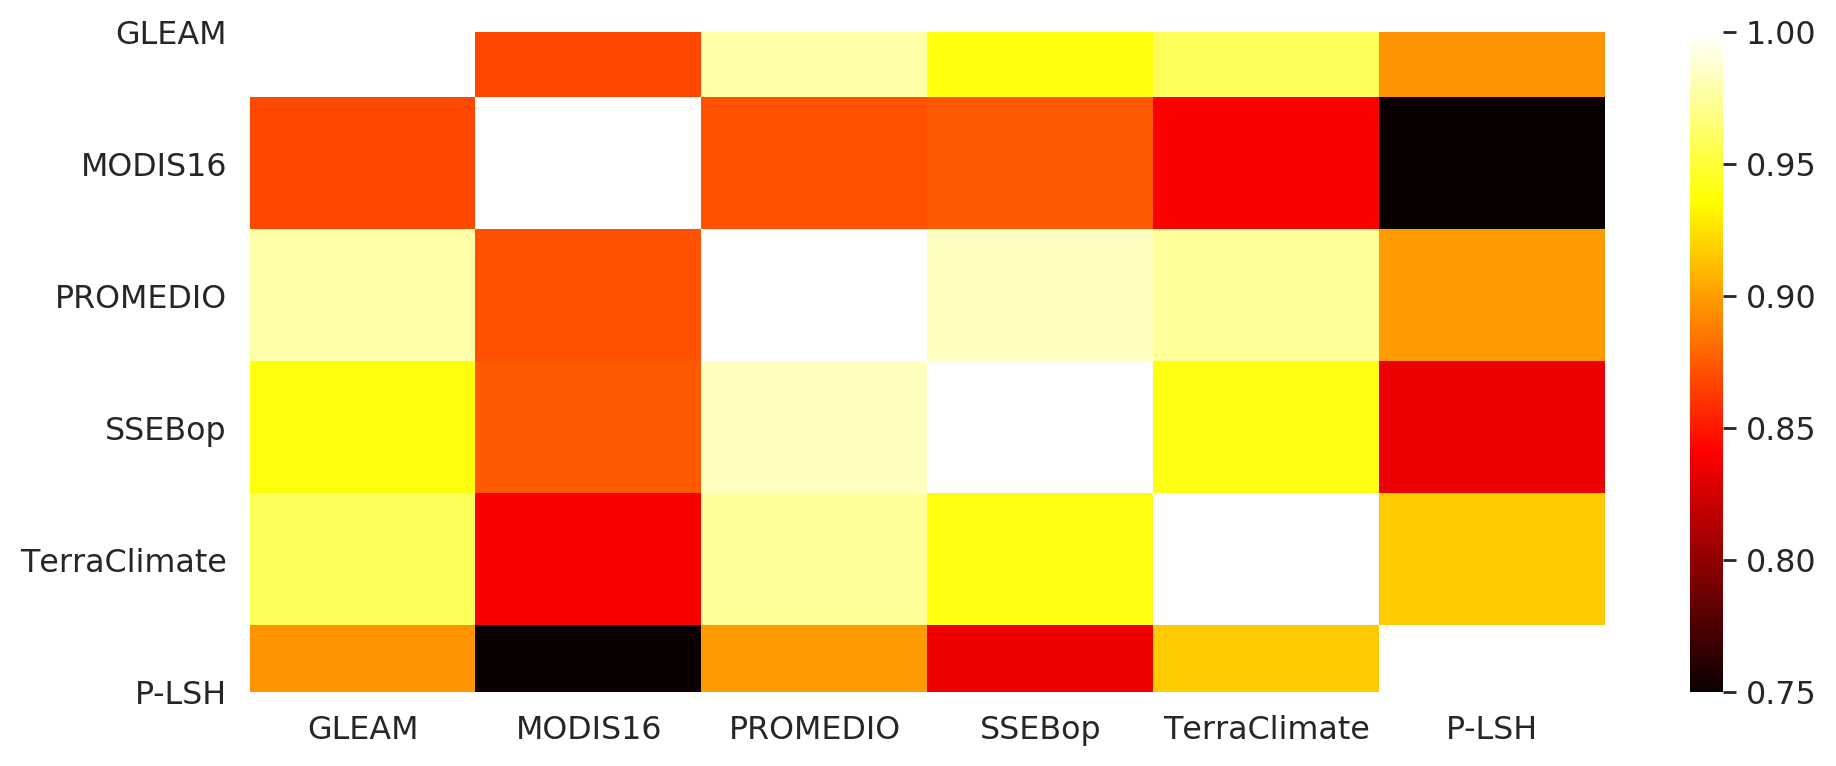
\includegraphics[scale=.7]{Images/03_Tindex_AEproducts.png}
	\centering
	\caption{Matriz Td.}
	\label{fig:03_Tindex_AEproducts}
\end{figure}


Para establecer correctamente que producto (GLEAM, MODIS16, MEAN, SSEBop, TerraClimate, Zhang) usar se hizo un ranqueo y posterior selección a través de una validación con datos de $AE$ observado inferido por balance hídrico y Budyko. Dos asunciones han sido establecidas para poder validar los productos globales de $AE$. El primero es que si no hay tendencia en el $AE$ inferido por balance hídrico en las cuencas de evaluación, entonces los promedios de $AE$ inferido puede compararse con el promedio de diferentes tiempos. La segunda asunción es que el balance hídrico puede ser simplificado a la Ecuación \ref{equ:bheq}, donde para escalas anuales a decadales, el cambio en el almacenamiento es insignificante.

La primera asunción seria factible siempre y cuando no haya tendencia en $AE$. Teniendo en cuenta el contexto del cambio climático (incremento de $T$), es entonces esperado que $AE$ aumente también, sin embargo, debido a la falta de información no se tiene consenso acerca de las causas e inclusive la dirección de la tendencias en $AE$ \citep{hobbins2004trends,cong2009does,wang2011trends,miralles2016wacmos,douville2013anthropogenic,zhang2016multi}. Adicionalmente, se tiene evidencia a escala global que existe una tendencia decreciente en la evaporación, lo cual es contrario a lo esperado, este fenómeno se llama la “paradoja de la evaporación". Lo anterior hace que sea aun mas debatible entender la variabilidad espacio-temporal de $AE$. A la fecha, en Perú no existe trabajos en tendencias de $AE$, esto probable a la escasa o nula información de $AE$ observado. Debido a que la primera asunción es discutible, la validación solo se realizo en un periodo común de información (2000-2014) por lo que efectos de tendencia fueron aplacados y porque no se comparo en otros periodos temporales.
%Sin embargo, estudios como el de () afirman que ha habido tendencias decrecientes en estimaciones globales de ET con las mayores contribuciones regionales en tendencia descendente en Australia y África austral. Por otro lado, () reporta un comportamiento inverso, estimaciones globales de AE presentan un aumento principalmente en Australia y África austral. Adicionalmente, otras investigaciones en tendencias globales de AE no llegan a un acuerdo común acerca de la causa y/o dirección de las tendencias ().

Con respecto a la segunda asunción, muchos estudios establecen el cambio en el almacenamiento como nulo a escala de cuencas para periodos temporales extensos \citep{Budyko1961,Fu1981,Zhang2008,Wang2014,Singh2015}. El cambio en el almacenamiento de agua ha sido recientemente evaluado por \citet{rodell2018emerging} mediante el uso del Gravity Recovery and Climate Experiment (GRACE) para el periodo 2002-2016. La tendencia encontrada para el caso del Perú es menos de 1cm/año (no significativo), entonces asumiendo que existe una contribución en las cuencas de evaluación esta representaría menos de 1\% al promedio anual de $AE$. Por lo tanto, la segunda asunción es aceptable. 

Las cuencas de evaluación donde se realizo la validación fueron 13 (Anexo 2 y 3). La diversidad es buena ya que se distribuye de norte a sur en las tres principales vertientes (Pacifico, Altiplano y Amazonas) y fueron de diversos tamaño. En base a la información del Anexo 3 se realizo los cálculos para inferir $AE$ observado, y en conjunto con sus valores a escala de cuenca de los productos globales de $AE$ se hizo la validación. A modo de resumen, la Tabla \ref{tab:Table_r_rmse_bias} muestra la eficiencia de los productos $AE$ en función de las métricas: correlación de Spearman (Rs), error cuadrático medio (RMSE) y el error simple (bias). Se aprecia que los productos de $AE$ global tiene alta relación con el $AE$ observado inferido (Rs $>$ 0.7), destacando principalmente GLEAM, MEAN, TerraClimate y MODIS16. Por otro lado, RMSE es muy variado para cada uno de los productos, se encontró mayor error por parte de SSEBop seguido por ZHANG. Los errores de SSEBop son debidos a la sub-estimación (bias negativo) por parte del producto global. Lo anterior, contrario para ZHANG, donde el bias es positivo. GLEAM destaca por tener los menores errores tanto bias como en RSME. Una inspección al bias considerando cada cuenca y producto global (Anexo 4) aclara lo anterior mencionado. MODIS16 y ZHANG (SEEBop) sobrestiman (subestiman) en prácticamente todas las cuencas de evaluación. MEAN y TerraClimate tienden a subestimar ligeramente. Solo GLEAM presento menos y próximos a 0 de bias en ciertas cuencas de evaluación.

\begin{table}[hbt]
\caption{Resumen de validación. BH: Balance Hídrico y BK: Budyko}
\label{tab:Table_r_rmse_bias}
\centering
\begin{tabular}{lllllll}
\hline
Productos    & \multicolumn{2}{l}{Rs} & \multicolumn{2}{l}{RMSE} & \multicolumn{2}{l}{bias} \\
Globales     & BH             & BK             & BH                   & BK                  & BH          & BK         \\  \hline
GLEAM        & 0.96           & 0.97           & 215.37               & 83.96               & -36.98      & 13.93      \\
MEAN         & 0.96           & 0.96           & 287.31               & 116.32              & -114.03     & -60.50     \\
MODIS16      & 0.96           & 0.96           & 232.81               & 186.18              & 124.88      & 193.45     \\
SSEBop       & 0.76           & 0.77           & 411.39               & 287.13              & -326.94     & -233.73    \\
TerraClimate & 0.97           & 0.98           & 355.14               & 141.36              & -126.68     & -94.51     \\
Zhang        & 0.84           & 0.85           & 400.20               & 365.50              & 323.86      & 354.15 \\ \hline    
\end{tabular}
\end{table}

Para el ranqueo de los productos globales de $AE$ se ordeno de mayor a menor (eficiencia) cada uno de las métricas de la Tabla \ref{tab:Table_r_rmse_bias} y se sumo los valores del orden. Por lo tanto, aquellos que tengan una puntuación mas baja reflejaría una mayor eficiencia de estimación de $AE$. La Tabla \ref{tab:Table_rank} muestra los resultados del ranqueo considerando el método de inferencia de $AE$ observado y métrica utilizada. 

\begin{table}[hbt]
\caption{Ranqueo de productos globales de AE}
\label{tab:Table_rank}
\begin{tabular}{llllllll}
\hline
\multirow{2}{*}{Métrica} & \multirow{2}{*}{Método} & \multicolumn{6}{l}{Productos}                          \\
                         &                             & GLEAM & MEAN & MODIS16 & SSEBop & TerraClimate & Zhang \\ \hline
Rs                       & BH                          & 2     & 3    & 3       & 5      & 1            & 4     \\
                         & BK                          & 2     & 3    & 3       & 5      & 1            & 4     \\
RMSE                     & BH                          & 1     & 3    & 2       & 5      & 4            & 6     \\
                         & BK                          & 1     & 2    & 4       & 5      & 3            & 6     \\
bias                     & BH                          & 1     & 2    & 3       & 6      & 4            & 5     \\
                         & BK                          & 1     & 2    & 4       & 5      & 3            & 6     \\
\multicolumn{2}{l}{Puntuación}                         & 8     & 15   & 19      & 31     & 16           & 31    \\
\multicolumn{2}{l}{Orden}                              & 1     & 2    & 4       & 5      & 3            & 5    \\ \hline
\end{tabular}
\end{table}

Es evidente de la Tabla \ref{tab:Table_rank} que los mejores productos fueron GLEAM, MEAN y TerraClimate y los menos eficientes SSEBop y ZHANG. Esto en concordancia con los resultados anteriormente discutidos. Sin embargo, este ranqueo solo esta basado en las métricas que caracteriza la magnitud de $AE$, mas no su resolución espacial y su capacidad de estimar $AE$ en tipos de suelos específicos tales como: cuerpos agua y/o áreas irrigadas. El reciente trabajo de \citet{Weerasinghe2019discuss} considera que este tipo de validación es pertinente, sin embargo no hay forma objetiva de hacer una clasificación por tipo de suelo, considerando que existe una diversidad de formas. Si tomamos en cuenta la resolución espacial de cada producto es evidente que GLEAM seria el mas afectado ya que es el producto con menor resolución (0.25$^{\circ}$ ). Esto no modificaría el orden que se le dio a GLEAM inicialmente, pero acercaría mas el resto de productos a una puntuación mas baja (mayor eficiencia). Los otros productos con aceptable eficiente y mayor resolución que GLEAM son MEAN y TerraClimate. Considerando el tamaño de cuenca hidrográfica a usar para el análisis de la vulnerabilidad de los RH (ANA), estos serian mas aceptables. El producto a destacar es MEAN ya que es el promedio del resto de productos de $AE$ los cuales son estimaciones independientes (cada producto tiene diferentes parametrizaciones y datos de entrada), entonces MEAN es la representación promedio de los ensembles de $AE$. A diferencia de usar un solo producto, es mas representativo usar el promedio ya que ningún producto sera completamente eficiente en todo el territorio. Una similar idea es dado por \citet{zhang2016review}, y ejemplificado por \citet{da2019spatial} donde se produce un producto de $AE$ para la cuenca Amazónica como el promedio de diversos producto de $AE$.

En consecuencia, GLEAM, MEAN y TerraClimate son los mejores productos de $AE$ ya que representan con menor error los valores inferidos de $AE$. Cada uno de estos tiene una resolución espacial y temporal especifica. Su selección debe estar basado en el tipo de pregunta científica a responder. Para esta investigación y para los posteriores análisis se establece a MEAN como el referente de $AE$.

\subsection{Budyko probabilístico}

Seleccionado $AE$ y $P$ (de PISCOp 2.1), solo es requerido $PE$ para la aplicación del Budyko probabilístico. $PE$ se obtuvo a partir de $Tx$ y $Tn$ (de PISCOt 1.1) usando la ecuación de \citet{Hargreaves1985}. Los $PE$ anuales se muestran en el Anexo 5. Una vez las tres variables ($AE$, $PE$ y $P$) establecidos se procedió a la extracción de sus valores climáticos a escala de UH del ANA. Los valores del índice de Evaporación ($AE/P$) y Aridez ($PE/P$) por cada UH se observan en el Anexo 6. 

El índice de evaporación presenta una variabilidad espacial menos coherente que el índice de aridez. En general $AE/P$ tiende a tener valores mayores a 1 en las UH cercanas a la franja costera y en algunas ubicadas en la vertiente del Amazonas. $PE/P$ varia de mayor a menor de oeste a este, respectivamente. Similar a $AE/P$, los valores mayores a 10 se encuentran prácticamente en la costa para ir disminuyendo mientras se desplaza a la vertiente del Amazonas, donde prácticamente tiene como valor de $\approx$2 en todo su contorno. Debido a que la ecuación de Budyko es solo aceptable bajo las leyes de suministro de agua atmosférica ($AE < P$) y de demanda ($AE < PE$), aquellas UH que no cumplieron fueron removidas del análisis (Figura \ref{fig:06_Ai_Ei_Omega_spatial}). Por esta remoción quedaron en total 18, 76 y 16 para la vertiente del Pacifico, Amazonas y Titicaca, respectivamente.

\clearpage %
\begin{sidewaysfigure}
	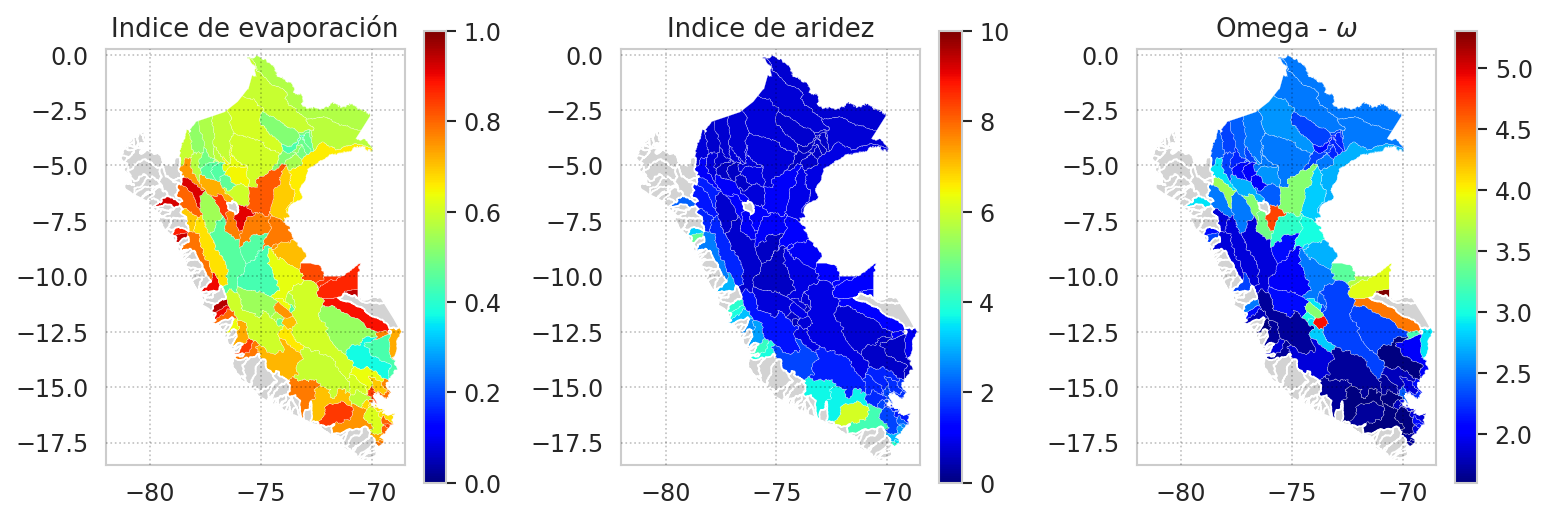
\includegraphics[scale=1]{Images/06_Ai_Ei_Omega_spatial.png}
	\centering
	\caption{Indice de evaporación ($AE/PE$) y de aridez ($PE/P$) climático (2000-2014) para las unidades hidrográficas del ANA omitiendo cuencas que violen las restricciones de Budyko (en gris). Adicionalmente, el parámetro $\omega$ calibrado.}
	\label{fig:06_Ai_Ei_Omega_spatial}
\end{sidewaysfigure}

\clearpage %

Una posible explicación de la mayor remoción de UH en la vertiente del Pacifico, es a causa del bajo o nulo valor de $P$ en estas (si $P$ tiende a 0, $AE/P$ seria indeterminado). Esto puede ser natural o también forzado por el propio producto PISCOp 2.1 \citep{Aybar2019}. Además, $AE$ puede estar sobre-estimado, sin embargo, considerando la diversidad de productos de $AE$ analizados, la mayoría presenta una magnitud similar en la zona costera (a excepción del GLEAM). De acuerdo a \citet{greve2016two}, las condiciones bajo las cuales el marco de Budyko no es valido pueden ocurrir, por ejemplo, por cambios en los términos de almacenamiento de agua, la humedad del suelo, agua subterránea o almacenamiento de nieve. También, debido al agua introducida por el cambio del paisaje, intervenciones humanas (irrigación) o cambios de fase dentro del sistema o suministrados por precipitación. Posibles soluciones a esta limitación de Budyko se han presentando en la literatura \citep{greve2016two,moussa2016budyko,fathi2019new}. Sin embargo, esto esta fuera de los objetivos de la presente investigación. 

\begin{figure}[htb]
	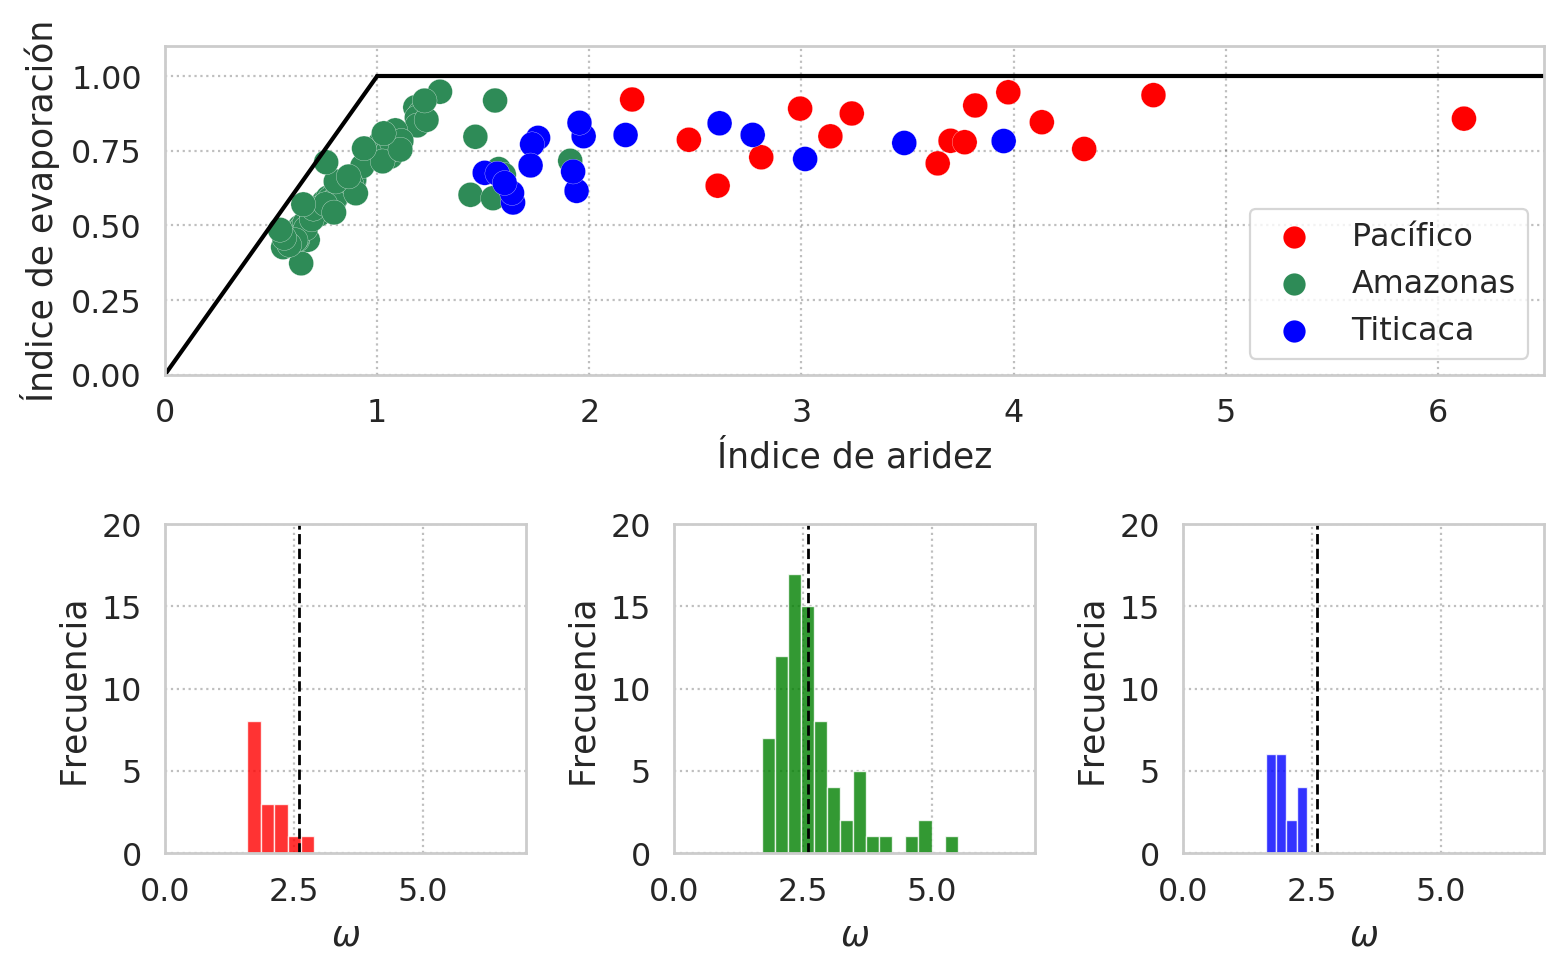
\includegraphics[scale=.78]{Images/07_Curve_and_omega.png}
	\centering
	\caption{Arriba) Ubicación de las UH en la curva de Budyko en función del índice de evaporación ($AE/P$) y aridez ($PE/P$). Abajo) Histogramas de la distribución del parámetro $\omega$ calibrado para cada UH y vertiente. La linea punteada en cada histograma indica el valor teórico de $\omega = 2.6$.}
	\label{fig:07_Curve_and_omega}
\end{figure}


La ubicación de las UH no removidas en la curva de Budyko se muestra en la Figura \ref{fig:07_Curve_and_omega}. Es muy fácil determinar la distinción de las UH por vertiente hidrográfica en la curva de Budyko. El parametro $\omega$ calibrado de Budyko oscila en el rango de 1.5 a 5.5 (Figura \ref{fig:06_Ai_Ei_Omega_spatial} y \ref{fig:07_Curve_and_omega}), presentándose los valores mas altos en la vertiente del Amazonas que en el Pacifico y Titicaca. Tomando en cuenta el valor teórico de $\omega = 2.6$ \citep{Fu1981}, solo en las UH de la vertiente del Amazonas, el $\omega$ calibrado se encuentra próximo (Figura \ref{fig:07_Curve_and_omega}). La agrupación de $\omega$ por vertiente hidrográfica es la representación de la distribución empírica de la misma. Entonces la distribución regional de $\omega$ es usada para poder estimar $AE/P$ en cada UH y obtener la incertidumbre asociada.

Después de obtener la distribución regional de $\omega$ (Figura \ref{fig:07_Curve_and_omega}), se realizo la validación cruzada de la eficiencia de la distribución empírica a escala nacional, de vertiente y UH. Como la distribución espacial de $\omega$ es en general uniforme ya que no presenta variaciones abruptas, los límites de incertidumbre resultantes de las agrupaciones basadas en la vecindad (es decir más cercanos) serán relativamente pequeños (Figura \ref{fig:06_Ai_Ei_Omega_spatial}), similar al estudio de \citet{Singh2015}. A diferencia de \citet{Greve2015}, quienes usaron la distribución de todas las cuencas para estimar $AE/P$ para cada cuenca. Es mas factible agrupar por regiones consideradas homogéneas.

\begin{table}[!ht]
\caption{Validación cruzada del parámetro $\omega$ a diferentes escalas.}
\label{tab:Table_pbias}
\centering
\begin{tabular}{lllllll}
\hline
\multirow{2}{*}{Escala} & \multirow{2}{*}{$PE/P$} & Observado & \multicolumn{3}{l}{Estimado ($AE/P$)} & Error  \\
                        &                       & ($AE/P$)    & 5\%        & 50\%       & 95\%      & (\%)   \\ \hline
Perú                    & 1.030                 & 0.667     & 0.482      & 0.658      & 0.805     & 1.383  \\
Pacífico                & 3.662                 & 0.825     & 0.720      & 0.823      & 0.950     & 0.177  \\
Amazonas                & 0.803                 & 0.596     & 0.498      & 0.603      & 0.713     & -1.236 \\
Titicaca                & 1.937                 & 0.748     & 0.603      & 0.727      & 0.812     & 2.830  \\ \hline
\end{tabular}
\end{table}


El bias porcentual de la mediana estimada en la validación cruzada oscila entre -1.2\% a 2.8\% del valor observado (Tabla \ref{tab:Table_pbias}). Asimismo, los valores regionales de $PE/P$ se encuentran dentro del rango 5\% y 95\% de estimación (Figura \ref{fig:09_proBK_val}). Una inspección mas a detalle del bias porcentual a escala de UH (Anexo 7) demuestra también el bajo error que oscila entre -20\% a 20\%. Solo las UH ubicadas al sur del Perú muestran un error mayor a -30\%. Se debe tener en cuenta que los valores son razones ($AE/P$), por lo que un error de ese rango es relativamente mínimo. Adicionalmente, esto es tomado en cuenta al tener la medida de incertidumbre en cada escala de análisis.

\begin{figure}[htb]
	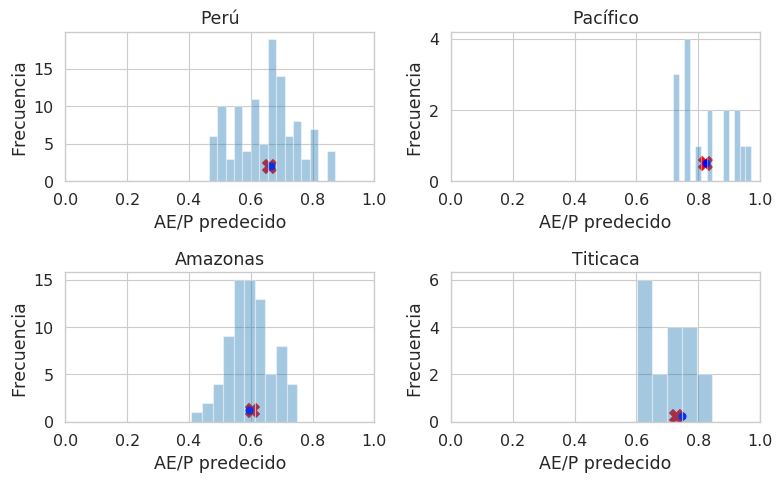
\includegraphics[scale=.78]{Images/09_proBK_val.png}
	\centering
	\caption{Validación del parámetro $\omega$ calibrado a escala de Perú y vertiente hidrográfica. Los histogramas muestran la distribución $AE/P$ predecido. El circulo representa el valor promedio observado de $AE/P$, y el aspa al promedio (de la distribución) de $AE/P$ predecido.}
	\label{fig:09_proBK_val}
\end{figure}


\subsection{Disponibilidad de los recursos hídricos debido al cambio climático}

Se estimo la vulnerabilidad de los RH al cambio climático para un rango de posibles escenarios (100 de $PE$ por 100 de $P$) a escala de Perú, vertiente hidrografica y de UH. De acuerdo al reporte de la IPCC, en América del Sur existe alta probabilidad de cambio de 1.5$^{\circ}$C a 8$^{\circ}$C y de -40\% a 40\%, para temperatura y precipitación respectivamente
\citep{stocker2013climate}. Esto en concordancia con las diferentes investigaciones en Perú, donde el aumento de temperatura es prácticamente un hecho \citep{vuille2015impact,rosas2016towards,lopez2016recent,vicente2018recent,hunziker2018effects} y el cambio en precipitación presenta mayor incertidumbre en su dirección y variabilidad espacial \citep{zubieta2017spatial,de2017can,Aybar2019}. Por lo tanto, para esta investigación los espacios climáticos se definen de la siguiente manera:

\begin{itemize}

	\item $\Delta P$ en -50\% a 50\%
	\item $\Delta PE$ en 0\% a 50\% (en función de $T$)

\end{itemize}

\begin{figure}[htb]
	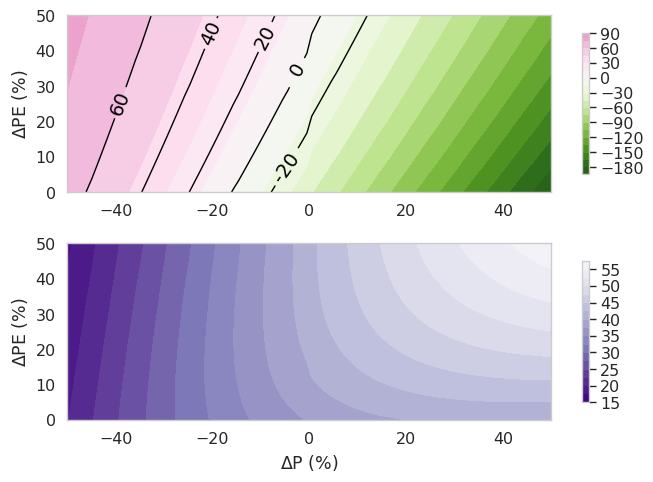
\includegraphics[scale=.8]{Images/12_VI_PERU_scale.png}
	\centering
	\caption{Arriba) Estimación de la vulnerabilidad de los RH (\%) a escala de Perú en función del cambio de precipitación ($\Delta P$) y evapotranspiración potencial ($\Delta PE$). Abajo) Incertidumbre (\%) de Arriba) en forma de desviación estándar. Se muestra isolineas de vulnerabilidad.}
	\label{fig:12_VI_PERU_scale}
\end{figure}


A escala de Perú, el índice de vulnerabilidad estimado ($VI$) y su incertidumbre asociada se presenta en la Figura \ref{fig:12_VI_PERU_scale}. Como era de esperarse, cambios negativos (positivos) de $P$ ($PE$) genero un aumento de la vulnerabilidad. Así como también, cambios en $P$ tuvieron un rol mayor que los cambios de $PE$ (en función de $T$), esto en linea con otros trabajos \citep{Singh2015}. La incertidumbre (debido al parámetro $\omega$) es mucho menor en los escenarios de aumento de vulnerabilidad que en los de disminución, como resultado de un escenario mas realista, y de acuerdo con otros estudios \citep{singh2011trading,Singh2015}.

A escala de vertiente hidrográfica, resultados similares a la Figura \ref{fig:12_VI_PERU_scale} se muestra en las Figuras \ref{fig:12_VI_Nivel_scale_Amazon}, \ref{fig:12_VI_Nivel_scale_Pacific} y \ref{fig:12_VI_Nivel_scale_Titicaca} para la vertiente del Amazonas, Pacifico y Titicaca, respectivamente. Se demuestra una vez mas la mayor influencia de $P$ para determinar la vulnerabilidad. Adicionalmente se evidencio que para un aumento de $VI$ en la vertiente del Amazonas se requiere un menor cambio de $P$, en comparación con el Pacífico y Titicaca (Figura \ref{fig:12_VI_Nivel_scale_Amazon}). Aunque la vertiente del Pacificó y Titicaca tuvieron un similar comportamiento de $VI$ en los espacios climáticos, la incertidumbre (vista como desviación estándar) es completamente diferente. Existe mayor incertidumbre (valores mas altos) en la vertiente del Pacífico, probablemente debido a la falta de muestra para construir la distribución de probabilidad empírica en esta región, es decir, menos cantidad de UH (Figuras \ref{fig:06_Ai_Ei_Omega_spatial}, \ref{fig:07_Curve_and_omega} y \ref{fig:12_VI_Nivel_scale_Pacific}). 


\begin{figure}[ht!]
	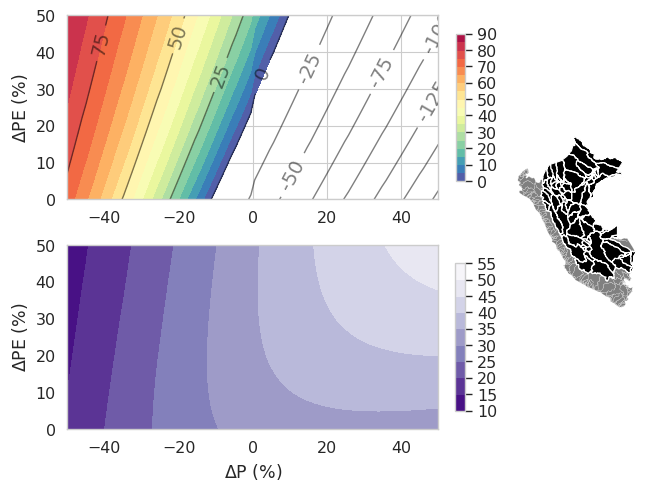
\includegraphics[scale=.85]{Images/12_VI_Nivel_scale_Amazon.png}
	\centering
	\caption{Similar a la Figura \ref{fig:12_VI_PERU_scale}, pero para la vertiente hidrográfica del Amazonas.}
	\label{fig:12_VI_Nivel_scale_Amazon}
\end{figure}


\begin{figure}[ht!]
	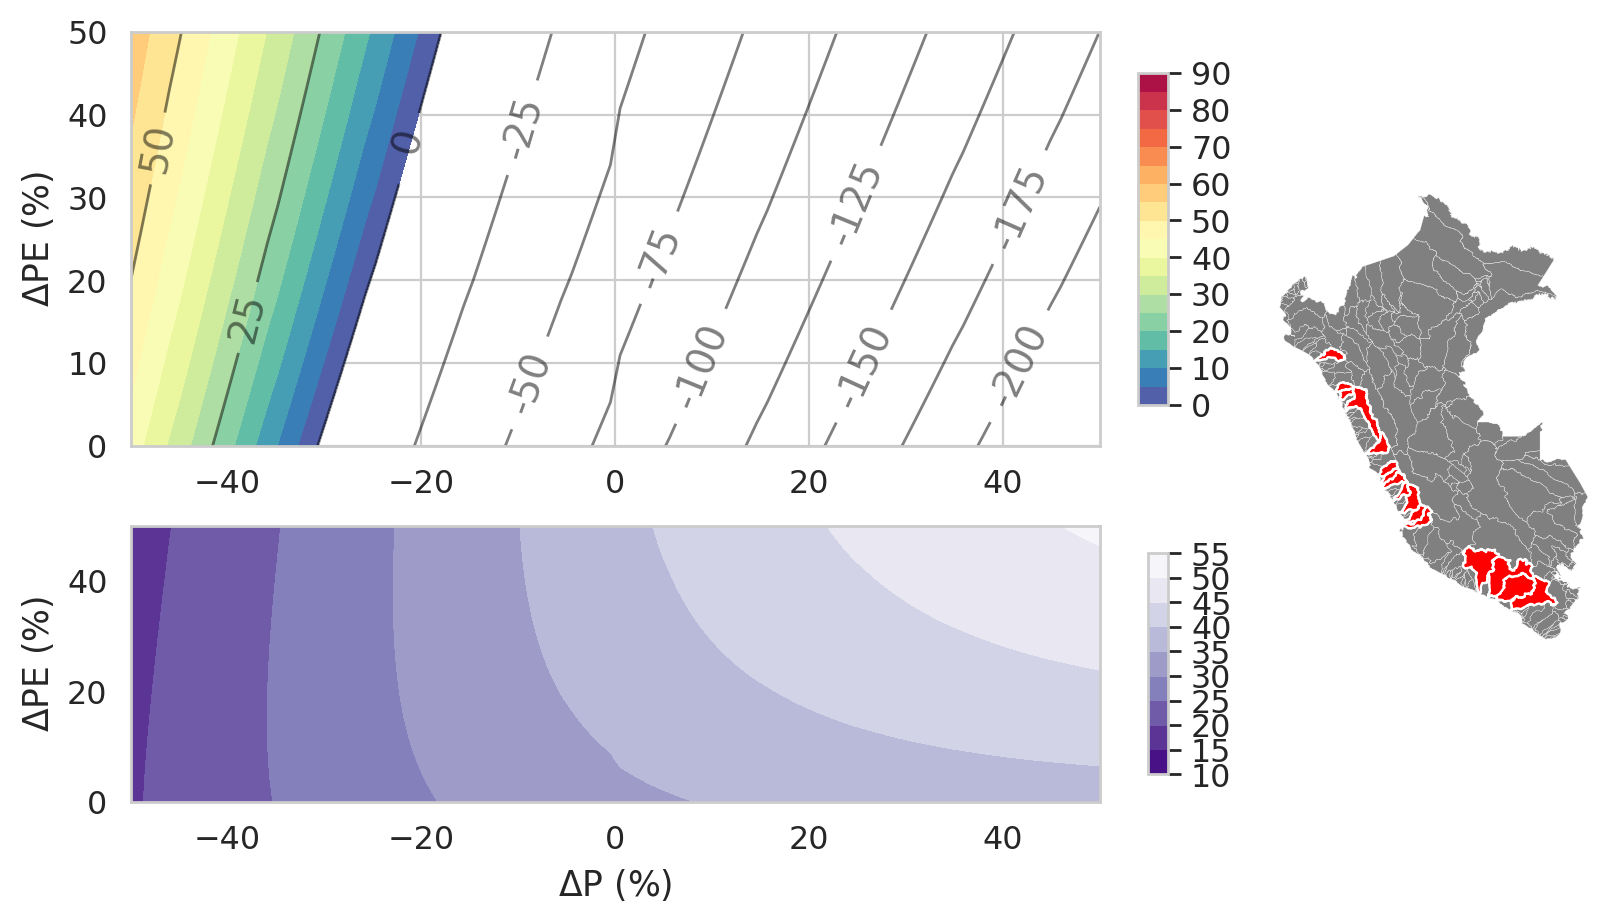
\includegraphics[scale=.75]{Images/12_VI_Nivel_scale_Pacific.png}
	\centering
	\caption{Similar a la Figura \ref{fig:12_VI_PERU_scale}, pero para la vertiente del Pacífico.}
	\label{fig:12_VI_Nivel_scale_Pacific}
\end{figure}



\begin{figure}[ht!]
	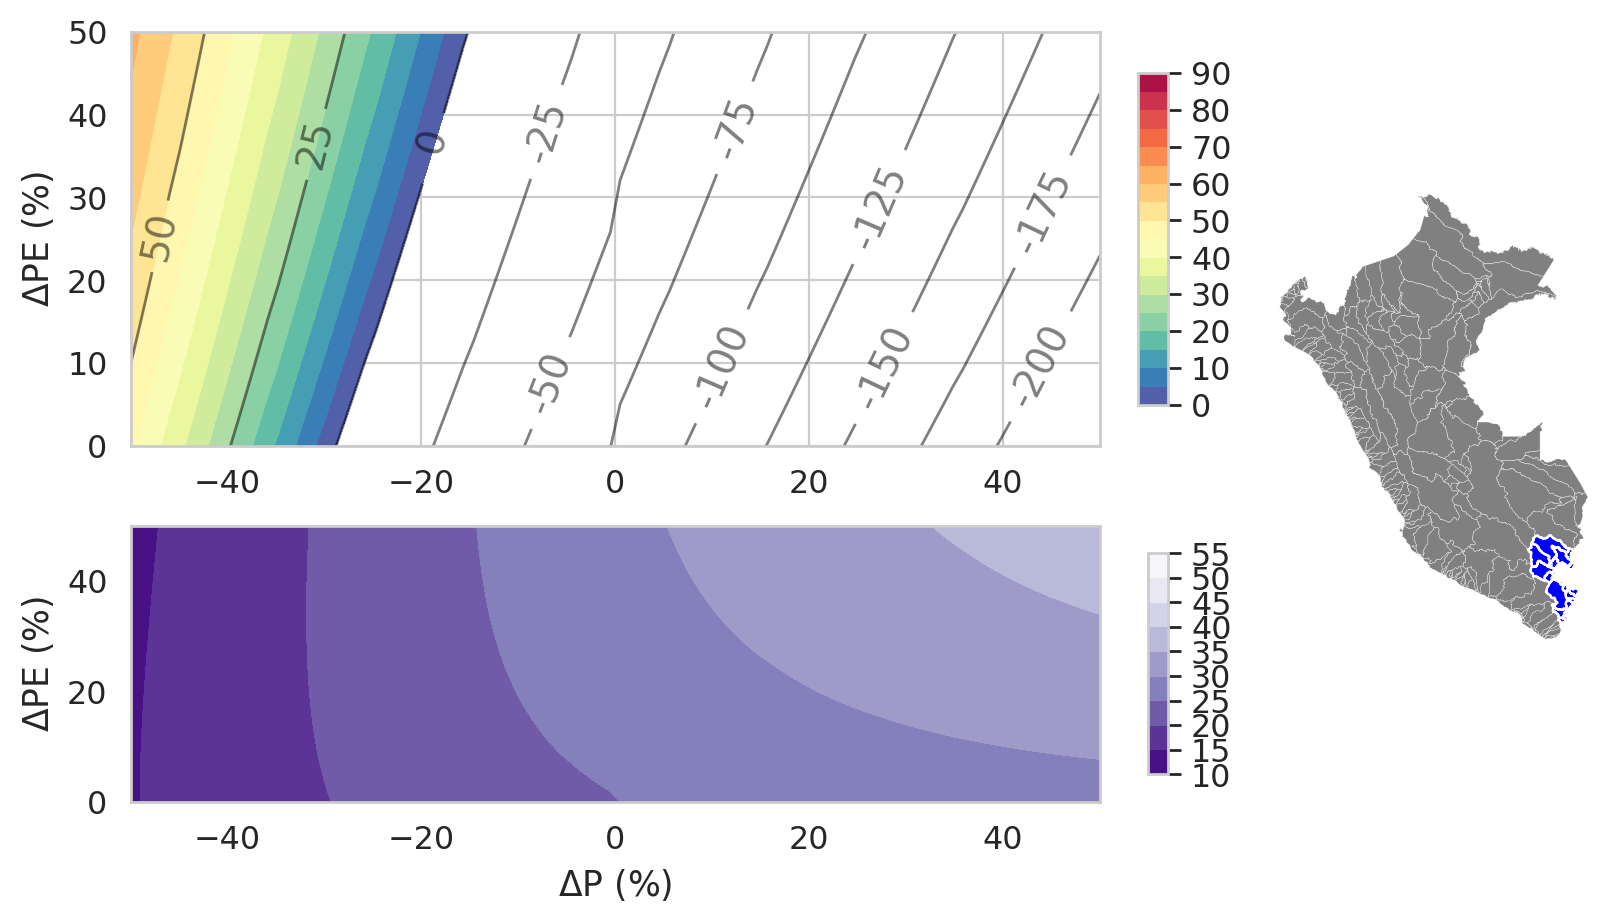
\includegraphics[scale=.75]{Images/12_VI_Nivel_scale_Titicaca.png}
	\centering
	\caption{Similar a la Figura \ref{fig:12_VI_PERU_scale}, pero para la vertiente del Titicaca.}
	\label{fig:12_VI_Nivel_scale_Titicaca}
\end{figure}



Para mayor detalle del análisis, se realizo el mismo procedimiento pero a escala de UH. El proceso puede ser entendido de la siguiente manera. En cada UH se tiene una matriz similar al de la Figura \ref{fig:12_VI_PERU_scale}, la cual se construyo en base a la distribución regional de $\omega$, perteneciente a una determinada vertiente. Entonces, es posible identificar umbrales críticos para un especifico valor de vulnerabilidad (y también para cambios en $PE$ y $P$) para cada UH y así poder visualizarlo en el espacio. A manera de ejemplo, la Figura \ref{fig:13_14figs} representa el $VI$ para cada UH cuando se tiene cambios de $P$ y $PE$ en un -20\% y 20\% respectivamente. Se evidencia un aumento critico de vulnerabilidad de hasta 50\% en UH ubicadas principalmente en toda la longitud de los Andes (cabeceras de cuenca), pero principalmente al sur-oeste (vertiente del Pacifico y Titicaca) y sur-este (vertiente del Amazonas) del Perú. La incertidumbre asociada para estas UH se encuentra dentro de una variación de 10-20\%. Otros escenarios puede ser fácilmente acoplados, por ejemplo, para un cambio de $PE$ en 20\% y un $VI$ de 25\%, el cambio critico de $P$ es prácticamente bajo en las UH de los Andes, principalmente las ubicadas al sur. Sin embargo, estos valores tiene una incertidumbre ligeramente mayor que el escenario anterior. Por lo tanto, un descubrimiento de esta investigación es que las UH ubicadas en las partes altas de los Andes (principalmente al sur de Perú) son los mas vulnerables lo que conduciría a aun aumento de su vulnerabilidad en el futuro. Las UH mas vulnerables para el caso de la Figura \ref{fig:13_14figs}a ($VI > 50\%$ e incertidumbre entre $10-20\%$) y \ref{fig:13_14figs}b ($\Delta P < 0\%$ e incertidumbre entre $10-30\%$): \textbf{Apurimac}, Camana, Carhuapanas, \textbf{Coata}, Crisnejas, (Alto) \textbf{Huallaga}, \textbf{Ilave}, \textbf{Ilpa}, \textbf{Inambari}, Mala, \textbf{Mantaro}, \textbf{Mauri}, Marañon, Pampas, Parananpura, \textbf{Perené}, \textbf{Pucara}, Tampobata y Urubamba (en negrita donde hubo coincidencia de ambos casos).

Aunque una disminución de -20\% en $P$ pueda ser exagerado, \citet{lausier2018overlooked} encuentra que existe tendencias decrecientes en la cola inferior y superior (de la distribución) que no necesariamente son consistentes con las de la media y mediana. Por lo tanto, previos trabajos pueden tener cierto grado de incertidumbre ya que solo se basan en la tendencia promedio de $P$. Para el caso de Perú, \citet{lausier2018overlooked} demuestra que existe concordancia en las tendencias de cola en un rango de -30mm a -50mm para el periodo 1950-2011, particularmente para el sur del Perú. Por consiguiente, escenarios como los planteados en esta tesis ya sean probablemente reales.

\begin{figure}[htb]
\centering
 \subfloat[]{%
 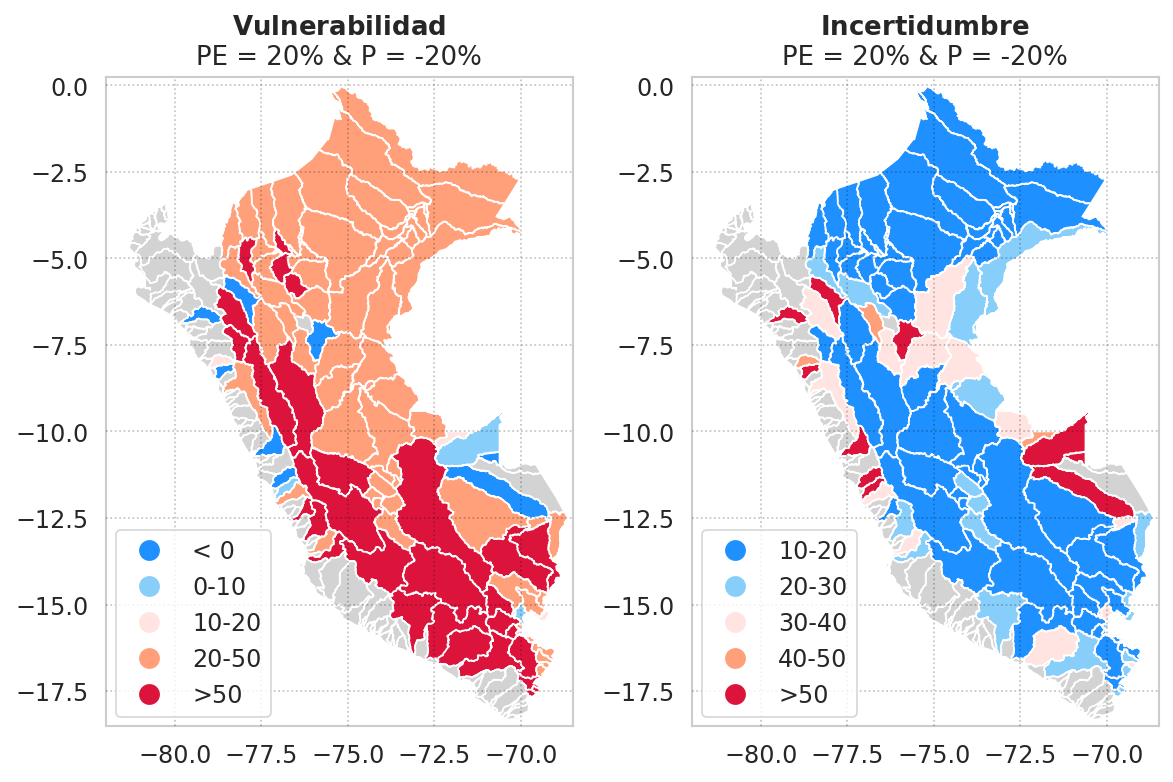
\includegraphics[scale=.75]{Images/13_VI_f(PE,P).png}} \hfill
 \subfloat[]{%
 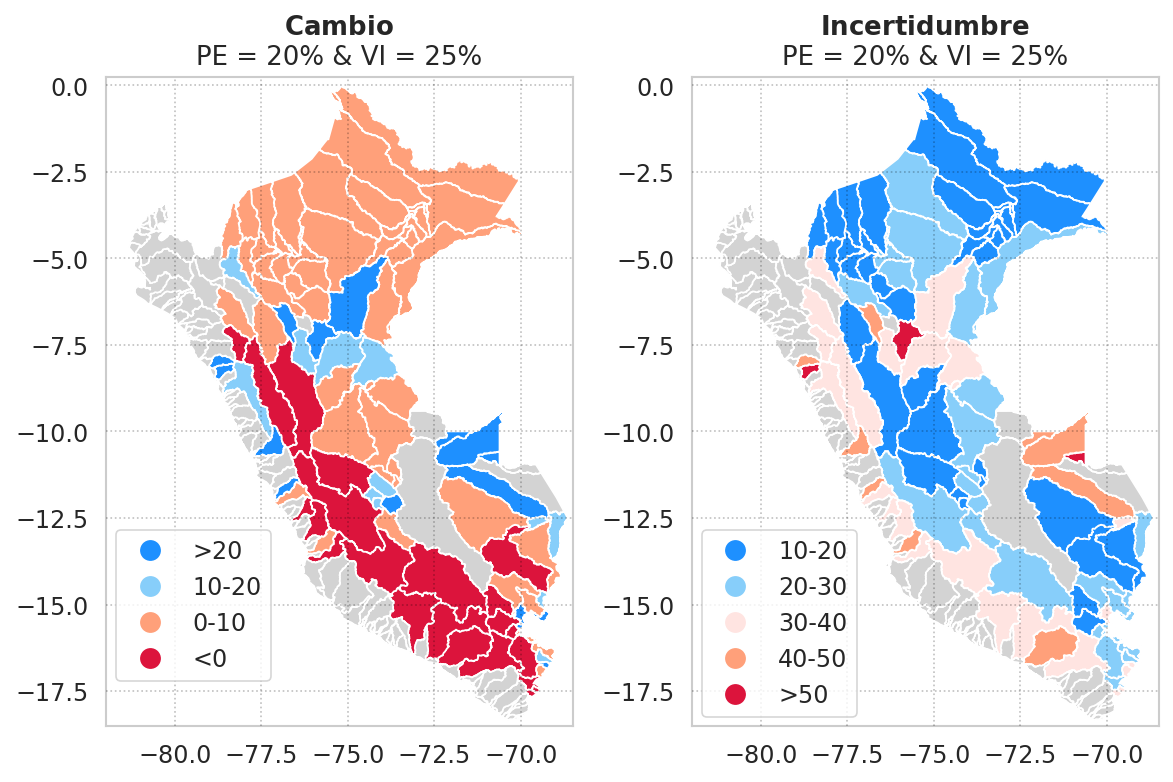
\includegraphics[scale=.75]{Images/14_P_f(PE,VI).png}} \hfill
 \caption{a) Variación espacial de $VI$ (\%) e incertidumbre (\%) asociada. b) Variación espacial del cambio critico de $P$ (\%) e incertidumbre (\%) asociada.}
 \label{fig:13_14figs}
\end{figure}


\clearpage
\vspace*{0.5mm}
\section{CONCLUSIONES}

\begin{itemize}
    \item \textbf{De selección de productos globales de evapotranspiración actual basada en percepción remota:} Se evaluó seis (mas el promedio de todos) productos evapotranspiración actual en conjunto con datos observados inferidos por balance hídrico y Budyko. La eficiencia de los productos en orden es: GLEAM, MEAN, TerraClimate, MODIS16, SSEBop y Zhang. Se recomienda el uso de los primeros productos de acuerdo al tipo de pregunta científica a responder debido a que cada uno de estos presenta una resolución espacial y temporal especifica. Para este trabajo de investigación se utilizo MEAN (promedio los productos).
   
    \item \textbf{De la aplicación del Budyko probabilístico:}
    Se demostró la eficiencia del Budyko probabilístico, no solo para estimar el índice de evaporación con un error mínimo aceptable, si no también para caracterizar la hidro-climatología a escala de cuenca, vertiente hidrográfica y en el territorio nacional. Esto principalmente para las vertientes del Amazonas y Titicaca. Se evidencio que enfoques deterministas de Budyko no necesariamente se ajustan a la realidad ($\omega = 2.6$)
    
    \item \textbf{De la estimación de la disponibilidad de los recursos hídricos e incertidumbre asociada frente al cambio climático:} El enfoque de espacios climáticos (“bottom-up") demostró ser de gran utilidad para poder estimar la vulnerabilidad de los recursos hídricos e incertidumbre asociada, sin necesidad de hacer uso de salidas de modelos globales de cambio climático. De acuerdo a los resultados, se requiere un cambio mínimo de precipitación (menor a 10\%) y se espera una mayor vulnerabilidad (25\%) para las cuencas ubicadas en la parte alta de los Andes (\textbf{Apurimac}, Camana, Carhuapanas, \textbf{Coata}, Crisnejas, (Alto) \textbf{Huallaga}, \textbf{Ilave}, \textbf{Ilpa}, \textbf{Inambari}, Mala, \textbf{Mantaro}, \textbf{Mauri}, Marañon, Pampas, Parananpura, \textbf{Perené}, \textbf{Pucara}, Tampobata y Urubamba), primordialmente aquellas ubicadas al sur del país. Es necesario priorizar estas áreas para eventuales estudios de desarrollo sostenible ante el cambio climático.
    
\end{itemize}


\clearpage
\vspace*{0.5mm}
\section{RECOMENDACIONES}

Los resultados obtenidos en la presente tesis proponen nuevas perspectivas de investigación y recomendaciones que se detallan a continuación:

\begin{itemize}

    \item Se hace un llamado en implementar los enfoques probabilísticos de Budyko en estudios de hidro-climatología.
    
    \item Hacer uso de una mayor cantidad de productos de evapotranspiración actual, no solo provenientes de información satelital y/o reanalisis, si no de modelos empíricos.
    
    \item Adicionar otras bases de datos de precipitación y temperatura, así como también otros métodos de estimación de evapotranspiración potencial.
    
    \item Implementar en la validación de productos globales de evapotranspiración actual, los diferentes tipos de suelo, ya que esto daría mayor certeza de la veracidad del producto para diferentes propósitos.
    
    \item Aplicar el Budyko probabilístico no solo con el enfoque “bottom-up", si no también desde “top-down" usando las salidas de modelos de cambio climático. Así también la mezcla de ambos enfoques.

    \item Implementar o agregar un parámetro que relacione la vegetación en el Budyko probabilístico. De esta manera poder tener mas variables de cambio y así caracterizar otras influencias de los recursos hídricos que no sean solo del clima.
    
    \item Realizar la validación de los productos globales de evapotranspiración a otras escalas temporales tales como anual y mensual. De igual manera con el Budyko probabilístico haciendo uso de mayor cantidad de parámetros.
    
    
\end{itemize}


\clearpage
\vspace*{0.5mm}
\section{REFERENCIAS BIBLIOGRÁFICAS}
\bibliographystyle{References/apalikeADR}
\bibliography{References/ref}


\clearpage
\vspace*{0.5mm}
%\newgeometry{left=30mm, right=25mm, bottom =25mm, top=50mm}
\section{ANEXOS}

\centering

\appendices{\hspace{0.6cm}Anexo 1 \hspace{0.1cm} Información de productos de AE.} 
\Large{\textbf {Anexo 1: Información de productos de AE.}}
\vspace*{2cm}
\begin{table}[htb]
\label{tab:Table_AE_products_source}
\centering
\begin{tabular}{ll}
\hline
Producto     & Fuente                                                                     \\ \hline
GLEAM        & \url{https://www.gleam.eu/#downloads}                   \\
MODIS16      & \url{https://bit.ly/2HlHEG9}  \\
SSEBop       & \url{https://earlywarning.usgs.gov/fews/product/458}      \\
TerraClimate & \url{http://www.climatologylab.org/terraclimate.html}     \\
P-LSH        & \url{http://files.ntsg.umt.edu/data/ET_global_monthly/} \\
\hline
\end{tabular}
\end{table}

\clearpage
\appendices{\hspace{0.6cm}Anexo 2 \hspace{0.1cm} Series de tiempo de caudal.} 
\Large{\textbf {Anexo 2: Series de tiempo de cuencas de evaluación.}}
\vspace*{2.5cm}
\begin{figure}[ht]
	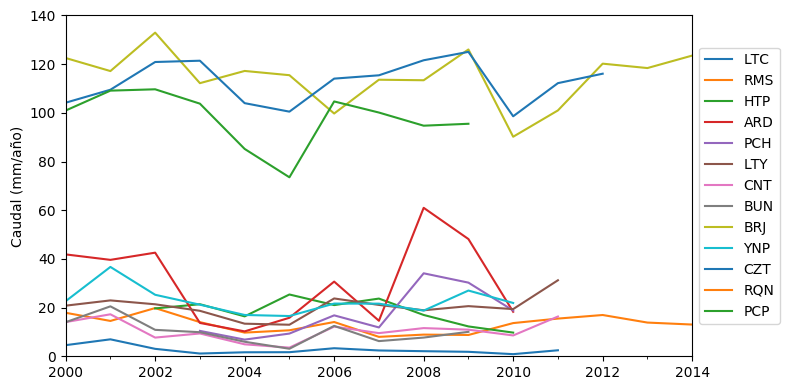
\includegraphics[scale=0.67]{Images/00_q_basins.png}
	\centering
	\label{fig:00_q_basins}
\end{figure}


\clearpage
\appendices{\hspace{0.6cm}Anexo 3 \hspace{0.1cm} Cuencas de evaluación.} 
\Large{\textbf {Anexo 3: Caracteristicas de cuencas de evaluación.}}
\vspace*{4cm}
\begin{table}[htb]
\label{tab:Table_q_area_basin}
\centering
\begin{tabular}{llllll}
\hline
No & Nombres      & Código & Área      & Caudal & Precipitación \\
   &              &        & (km2)       & (mm/año) & (mm/año)        \\ \hline
1  & La Tranca    & LTC    & 2021.13   & 32.42   & 169.69        \\
2  & Puente Ramis & RMS    & 15250.55  & 161.62  & 746.14        \\
3  & Huatiapa     & HTP    & 13007.90  & 225.06  & 511.15        \\
4  & Ardilla      & ARD    & 11996.54  & 372.07  & 766.24        \\
5  & Puchaca      & PCH    & 730.79    & 243.43  & 533.04        \\
6  & Letrayoc     & LTY    & 3465.36   & 248.46 & 457.49        \\
7  & Conta        & CNT    & 3049.04   & 127.63  & 375.61        \\
8  & Bella Union  & BUN    & 4287.02   & 122.01  & 280.01        \\
9  & Borja        & BRJ    & 114470.99 & 1397.81 & 1263.52       \\
10 & Yanapampa    & YNP    & 4193.84   & 276.72  & 455.83        \\
11 & Chazuta      & CZT    & 69004.69  & 1375.89 & 1891.09       \\
12 & Requena      & RQN    & 91122.63  & 3904.40 & 1813.54       \\
13 & Pucallpa     & PCP    & 265821.78 & 1193.29  & 1503.72      \\ \hline
\end{tabular}
\end{table}

\clearpage
\appendices{\hspace{0.6cm}Anexo 4 \hspace{0.1cm} bias en función de cuenca de evaluación y producto global.} 

\Large{\textbf {Anexo 4: bias en función de cuenca de evaluación y producto global.}}
\vspace*{3.5cm}

\begin{figure}[htb]
	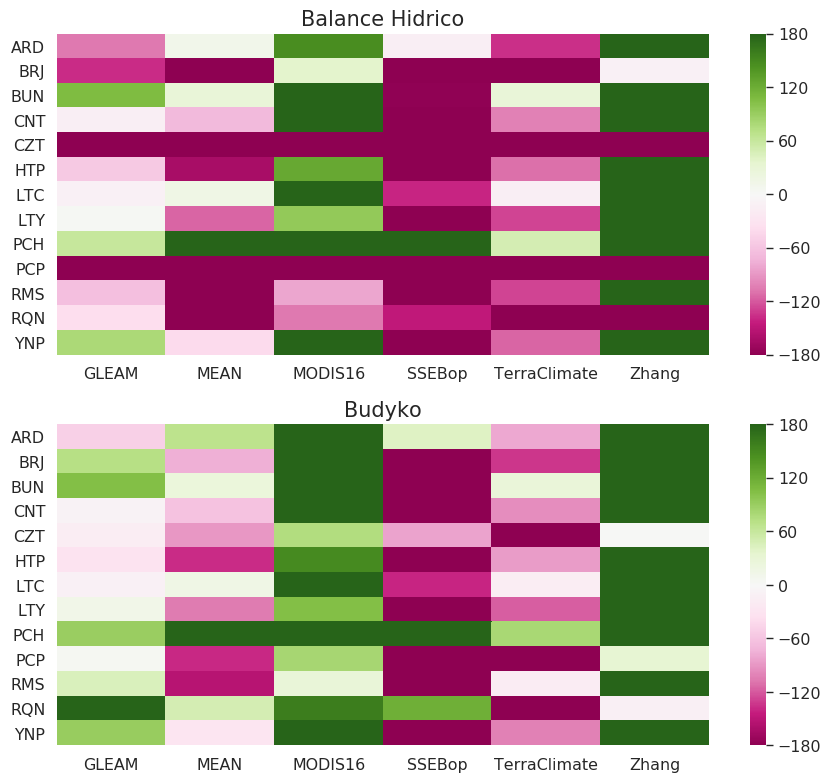
\includegraphics[scale=.7]{Images/04_BIAS_by_basin.png}
	\centering
	\label{fig:04_BIAS_by_basin}
\end{figure}


\clearpage
\appendices{\hspace{0.6cm}Anexo 5 \hspace{0.1cm} Calculo de la evapotranspiración potencial.} 

\Large{\textbf {Anexo 5: Calculo de la evapotranspiración potencial.}}
\vspace*{1.5cm}

\begin{figure}[ht]
\centering
	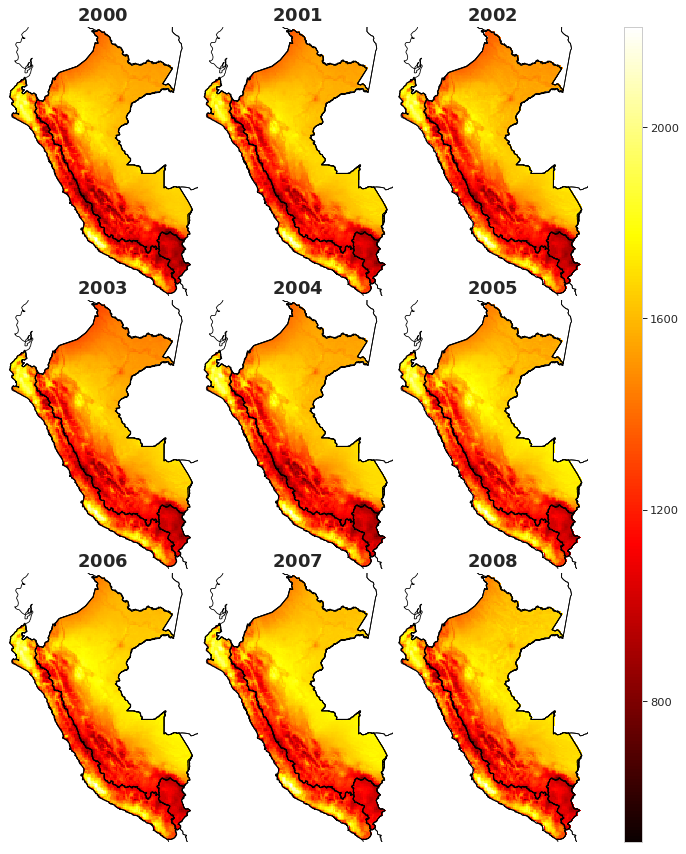
\includegraphics[width=15cm]{Images/01_PET_from_PISCOt.png}
	\label{fig:01_PET_from_PISCOt}
\end{figure}


\clearpage
\appendices{\hspace{0.6cm}Anexo 6 \hspace{0.1cm} Índice de evaporación y de aridez a escala de UH.} 

\Large{\textbf {Anexo 6: Índice de evaporación y de aridez a escala de UH.}}
\vspace*{1.5cm}
\begin{figure}[ht]
\centering
	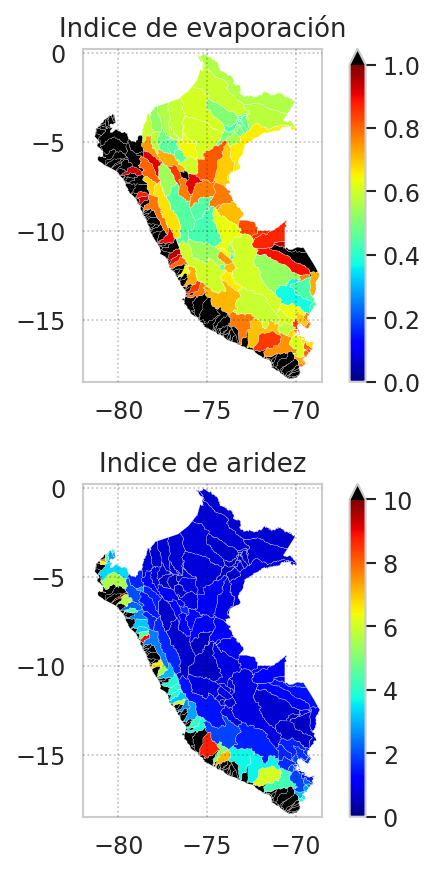
\includegraphics[scale=1.3]{Images/05_Ai_Ei_spatial.png}
	\label{fig:05_Ai_Ei_spatial}
\end{figure}


\clearpage
\appendices{\hspace{0.6cm}Anexo 7 \hspace{0.1cm} Bias porcentual del Budyko calibrado por cada UH.} 
\Large{\textbf {Anexo 7: Bias porcentual del Budyko calibrado por cada UH.}}
\vspace*{2.5cm}
\begin{figure}[ht]
\centering
	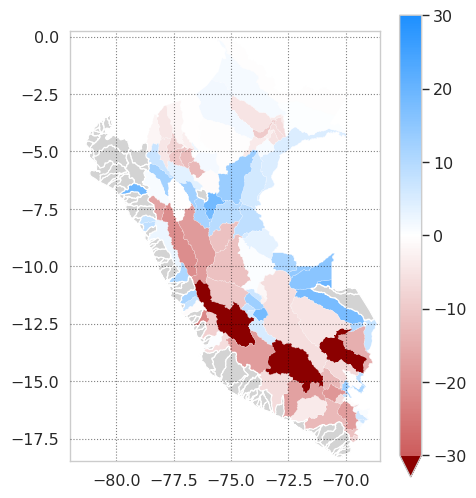
\includegraphics[scale=1.3]{Images/10_proBK_basin_by_nivel.png}
	\label{fig:10_proBK_basin_by_nivel}
\end{figure}


\end{document}